\documentclass[11pt,a4paper]{report}
\usepackage{hyperref}
\usepackage[margin=2.5cm]{geometry}
\usepackage{amsmath, amsthm}
\usepackage{txfonts}
\usepackage{todonotes}
\usepackage{enumitem}
\usepackage{listings}
\usepackage[nameinlink]{cleveref}
\usepackage{microtype}

\hypersetup{
  pdftitle={The Cardano Consensus and Storage Layer},
  pdfborder={0 0 0},
  breaklinks=true
}

\usetikzlibrary{arrows.meta}
\usetikzlibrary{intersections}

% https://tex.stackexchange.com/questions/229940/can-i-have-a-listing-with-fixed-column-code-and-full-flexible-comments
\makeatletter
\let\commentfullflexible\lst@column@fullflexible
\makeatother

% Use continuous footnote numbering so we can refer to them
% https://tex.stackexchange.com/questions/10448/continuous-footnote-numbering
\counterwithout{footnote}{chapter}

\lstset{
    language=haskell
  , basicstyle=\small\ttfamily
  , keywordstyle=\bfseries
  , commentstyle=\normalsize\rmfamily\itshape\commentfullflexible
  , columns=fixed
  , morekeywords={
        family
      , Type
      }
  }

\theoremstyle{definition}
\newtheorem{property}{Property}
\newtheorem{definition}{Definition}
\newtheorem{lemma}{Lemma}
\newtheorem{assumption}{Assumption}
\newtheorem{corollary}{Corollary}
\newtheorem{proposal}{Proposal}
\numberwithin{property}{chapter}
\numberwithin{definition}{chapter}
\numberwithin{lemma}{chapter}
\numberwithin{assumption}{chapter}
\numberwithin{corollary}{chapter}
\numberwithin{proposal}{chapter}

\newenvironment{bug}
  {\begin{quote} \textbf{Known bug}.}
  {\end{quote}}

\title{The Cardano Consensus and Storage Layer \\
       {\large \sc An IOHK technical report}
  }
\author{Edsko de Vries \\ \href{mailto:edsko@well-typed.com}
                               {\small \texttt edsko@well-typed.com}
   \and Thomas Winant  \\ \href{mailto:thomas@well-typed.com}
                               {\small \texttt thomas@well-typed.com}
   \and Duncan Coutts  \\ \href{mailto:duncan@well-typed.com}
                               {\small \texttt duncan@well-typed.com}
                       \\ \href{mailto:duncan.coutts@iohk.io}
                               {\small \texttt duncan.coutts@iohk.io}
  }

\newcommand{\debugsep}[1]{
  \vspace{2em}
  \hrule
  \vspace{0.5em}
  \textbf{#1}
  \vspace{0.5em}
  \hrule
  \vspace{2em}
}

% TODO
%
% * Incorporate
%
%   - Previous blog posts
%   - Specifications currently stored as markdown files in the repo
%   - Any discussions in long comments in the code
%
% - choice of k: liveness versus safety
% - make sure we talk about the fact that the ledger can be linear

\newcommand{\duncan}{\todo{Duncan suitable section.}}

\begin{document}

\maketitle

\tableofcontents

\chapter{Introduction}

The Cardano Consensus and Storage layer, or \emph{the consensus layer} for
short, is a critical piece of infrastructure in the Cardano Node. It
orchestrates between the \emph{network layer} below it and the
\emph{ledger layer} above it.

The network layer is a highly concurrent piece of software that deals with
low-level concerns; its main responsibility is to transmit data efficiently
across the network. Although it primarily transmits blocks and block headers, it
does not interpret them and does not need to know much about them. In the few
cases where it \emph{does} need to make some block-specific decisions, it
calls back into the consensus layer to do so.

The ledger layer by contrast exclusively deals with high-level concerns. It is
entirely stateless: its main responsibility is to define a single pure
function describing how the ledger state is transformed by blocks (verifying
that blocks are valid in the process). It is only concerned with linear history;
it is not aware of the presence of multiple competing chains or the roll backs
required when switching from one chain to another. We do require that the ledger
layer provides limited \emph{lookahead}, computing (views on near)
\emph{future} ledger states (required to be able to validate block headers
without access to the corresponding block bodies)

The consensus layer mediates between these two layers. It includes a
bespoke storage layer that provides efficient access to the current ledger state
as well as recent \emph{past} ledger states (required in order to be able
to validate and switch to competing chains). The storage layer also
provides direct access to the blocks on the blockchain itself, so that they can
be efficiently streamed to clients (via the network layer). When there are
competing chains, the consensus layer decides which chain is preferable and
should be adopted, and it decides when to \emph{contribute} to the chain
(produce new blocks). All ``executive decisions'' about the chain are made in
and by the consensus layer.

Lastly, as well we see, the consensus layer is highly abstract and places a
strong emphasis on compositionality, making it usable with many different
consensus algorithms and ledgers. Importantly, compositionality enables the
\emph{hard fork combinator} to combine multiple ledgers and regard them as a
single blockchain.

The goal of this document is to outline the design goals for the consensus
layer, how we achieved them, and where there is still scope for improvement. We
will both describe \emph{what} the consensus layer is, and \emph{why} it is the
way it is. Throughout we will also discuss what \emph{didn't} work, approaches
we considered but rejected, or indeed adopted but later abandoned; discussing
these dead ends is sometimes at least as informative as discussing the solution
that did work.

We will consider some of the trade-offs we have had to make, how they
affected the development, and discuss which of these trade-offs should perhaps
be reconsidered. We will also take a look at how the design can scale to
facilitate future requirements, and which requirements will be more problematic
and require more large-scale refactoring.

The target audience for this document is primarily developers working on the
consensus layer. It may also be of more broader interest to people generally
interested in the Cardano blockchain, although we will assume that the
reader has a technical background.

\chapter{Overview}
\label{storage}

\section{Components}
\label{storage:components}

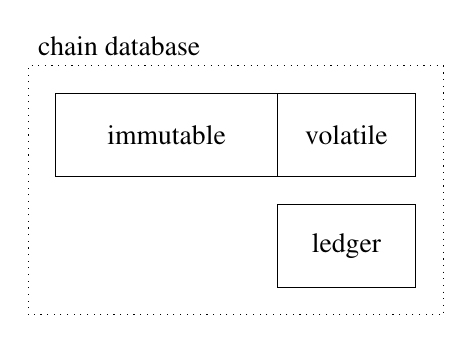
\begin{tikzpicture}
\draw [dotted]
     (-50pt, -65pt)
  -- ++(0, 90pt) node[above right] {chain database}
  -- ++(150pt, 0)
  -- ++(0, -90pt)
  -- cycle;
\node [draw, shape=rectangle, minimum width=80pt, minimum height=30pt] at (0,0)  {immutable};
\node [draw, shape=rectangle, minimum width=50pt, minimum height=30pt] at (65pt, 0)  {volatile};
\node [draw, shape=rectangle, minimum width=50pt, minimum height=30pt] at (65pt, - 40pt) {ledger};
\end{tikzpicture}

Discuss the immutable/volatile split (we reference this section for that).

\section{In memory}
\label{storage:inmemory}

TODO: After we discussed the overview, we should give an overview of everything
we store in memory in any component, so that we have a better understanding of
memory usage of the chain DB as a whole.

\subsection{Chain fragments}
\label{storage:fragments}

\subsection{Extended ledger state}
\label{storage:extledgerstate}
\label{storage:headerstate}

TODO: Is there a more natural place to talk about this? Introducing the
header state when introducing the storage layer does not feel quite right.
The storage layer might be storing the header state, but that doesn't
explain its existence.

ChainDepState, (ChainIndepState), LedgerState, ExtLedgerState

\chapter{Non-functional requirements}
\label{nonfunctional}

This whole chapter is Duncan-suitable :)
\duncan

\section{Network layer}
\label{nonfunctional:network}

This report is not intended as a comprehensive discussion of the network layer;
see \cite{network-spec} instead. However, in order to understand
some of the design decisions in the consensus layer we need to understand some
of the requirements imposed on it by the network layer.

TODOs:

\begin{itemize}
\item Highlight relevant aspects of the design of the network layer
\item Discuss requirements this imposes on the consensus layer
Primary example: Forecasting.
\item How do we keep the overlap between network and consensus as small
as possible? Network protocols do not involve consensus protocols
(chain sync client is not dependent on chain selection). Chain sync
client + "pre chain selection" + block download logic keeps things isolated.
\item Why do we even want to validate headers ahead of time? (Thread model etc.)
(Section for Duncan?).
Section with a sketch on an analysis of the amortised cost for attackers versus
our own costs to defend against it ("budget for work" that grows and shrinks
as you interact with a node).
\end{itemize}

\subsection{Header/Body Split (aka: Header submission)}
\label{nonfunctional:network:headerbody}

Discuss the chain fragments that we store per upstream node.
Discuss why we want to validate headers here -- without a full ledger state
(necessarily so, since no block bodies -- can't update ledger state): to prevent
DoS attacks.
(\cref{ledger:forecasting} contains a discussion of this from the point of view of
the ledger).
Forward reference to the chain sync client (\cref{chainsyncclient}).
Discuss why it's useful if the chain sync client can race ahead  for
\emph{performance} (why it's required for chain selection is the discussed in
\cref{forecast:ledgerview}).

See also section on avoiding the stability window
(\cref{low-density:pre-genesis}).

\subsection{Block submission}
\label{nonfunctional:network:blocksubmission}

Forward reference to \cref{servers:blockfetch}.

\subsection{Transaction submission}
\label{nonfunctional:network:txsubmission}

Mention that these are defined entirely network side, no consensus involvement
(just an abstraction over the mempool).

\section{Security "cost" concerns}

TODO: Look through the code and git history to find instances of where we
one way but not the other because it would give an attacker an easy way to
make it do lots of work (where were many such instances).

Fragile. Future work: how might be make this less brittle?
Or indeed, how might we test this?

Counter-examples (things we don't want to do)

\begin{itemize}
\item Parallel validation of an entire epoch of data (say, crypto only).
You might do a lot of work before realising that that work was not needed because
of an invalid block in the middle.
\end{itemize}

Future work: opportunities for parallelism that we don't yet exploit
(important example: script evaluation in Goguen).

\section{Hard time constraints}

Must produce a block on time, get it to the next slot leader

Bad counter-example: reward calculation in the Shelley ledger bad
(give examples of why).

\section{Predictable resource requirements}

make best == worst

(not \emph{just} a security concern: a concern even if every node honest)


\part{Consensus Layer}

\chapter{Consensus Protocol}
\label{consensus}

% TODO: what kind of variation does this design support?
% (counter-example: genesis rule)

% TODO: Describe API
%
% TODO: State invariants
%
% TODO: Discuss relationship to the Ouroboros papers. Where are the various parts
% of the paper implemented? How do additional design constraints change this?
% (e.g. header/body split)

\section{Overview}

\subsection{Chain selection}
\label{consensus:overview:chainsel}

Chain selection is the process of choosing between multiple competing chains,
and is one of the most important responsibilities of a consensus protocol. When
choosing between two chains, in theory any part of those chains could be
relevant; indeed, the research literature typically describes chain selection as
a comparison of two entire chains (\cref{bft-paper,praos-paper}). In practice
that is not realistic: the node has to do chain selection frequently, and
scanning millions of blocks each time to make the comparison is of course out of
the question.

The consensus layer keeps the most recent headers as a \emph{chain fragment}
in memory (\cref{storage:inmemory}); the rest of the chain is stored on disk.
Similarly, we keep a chain fragment of headers in memory for every (upstream)
node whose chain we are following and whose blocks we may wish to adopt
(\cref{chainsyncclient}). Before the introduction of the hard fork combinator
chain selection used to be given these fragments to compare; as we will discuss
in \cref{hfc:intro}, however, this does not scale so well to hybrid chains.

It turns out, however, that it suffices to look only at the headers at the very
tip of the chain, at least for the class of consensus algorithms we need to
support. The exact information we need about that tip varies from
one protocol to the other, but at least for the Ouroboros family of consensus
protocols the essence is always the same: we prefer longer chains over shorter
ones (justifying \emph{why} this is the right choice is the domain  of
cryptographic research and well outside the scope of this report). In the
simplest case, the length of the chain is \emph{all} that matters, and hence the
only thing we need to know about the blocks at the tips of the chains is their
block numbers.\footnote{This is not \emph{entirely} true, due to the presence of
EBBs; see \cref{ebb-chain-selection}.}

This does beg the question of how to compare two chains when one (or both) of
them are empty, since now we have no header to compare. We will resolve this by
stating the following fundamental assumption about \emph{all} chain selection
algorithms supported by the consensus layer:

\begin{assumption}[Prefer extension]
\label{prefer-extension}
The extension of a chain is always preferred over that chain.
\end{assumption}

A direct consequence of \cref{prefer-extension} is that a non-empty chain is
always preferred over an empty one,\footnote{Comparing empty chain
\emph{fragments}, introduced in \cref{storage:fragments}, is significantly more
subtle, and will be discussed in \cref{chainsel:fragments}.} but we will
actually need something stronger than that: we insist that shorter chains can
never be preferred over longer ones:

\begin{assumption}[Never Shrink]
\label{never-shrink}
A shorter chain is never preferred over a longer chain.
\end{assumption}

\Cref{never-shrink} does not say anything about chains of equal length; this will
be important for Praos (\cref{praos}). An important side-note here is that
the Ouroboros Genesis consensus protocol includes a chain selection rule
(the genesis rule) that violates \cref{never-shrink} (though not \cref{prefer-extension}); it also cannot be defined by only looking at the tips of chains.
It will therefore require special treatment; we will come back to this in
\cref{genesis}.

\subsection{The security parameter $k$}
\label{consensus:overview:k}

TODO\todo{TODO}.

\section{The \lstinline!ConsensusProtocol! Class}
\label{consensus:class}

We model consensus protocols as a single class called
\lstinline!ConsensusProtocol!; this class can be considered to be the
central class within the consensus layer.

\begin{lstlisting}
class (..) => ConsensusProtocol p where
\end{lstlisting}

The type variable $p$ is a type-level tag describing a particular consensus
protocol; if Haskell had open kinds\footnote{We will come back to this in
\cref{future:openkinds}.}, we could say \lstinline!(p :: ConsensusProtocol)!.
All functions within this class take an argument of type
%
\begin{lstlisting}
data family ConsensusConfig p :: Type
\end{lstlisting}
%
This allows the protocol to depend on some static configuration data; what
configuration data is required will vary from protocol to
protocol.\footnote{Explicitly modelling such a required context could be avoided
if we used explicit records instead of type classes; we will discuss this point
in more detail in \cref{technical:classes-vs-records}.}  The rest of the
consensus layer does not really do much with this configuration, except make it
available where required; however, we do require that whatever the configuration
is, we can extract $k$ from it:
%
\begin{lstlisting}
protocolSecurityParam :: ConsensusConfig p -> SecurityParam
\end{lstlisting}
%
For example, this is used by the chain database to determine when blocks can be
moved from the volatile DB to the immutable DB (\cref{storage:components}). In
the rest of this section we will consider the various parts of the
\lstinline!ConsensusProtocol! class one by one.

\subsection{Chain selection}
\label{consensus:class:chainsel}

As mentioned in \cref{consensus:overview:chainsel}, chain selection will only
look at the headers at the tip of the ledger. Since we are defining consensus
protocols independent from a concrete choice of ledger, however
(\cref{decouple-consensus-ledger}), we cannot use a concrete block or header
type. Instead, we merely say that the chain selection requires \emph{some} view
on headers that it needs to make its decisions:

\begin{lstlisting}
type family SelectView p :: Type
type SelectView p = BlockNo
\end{lstlisting}

The default is \lstinline!BlockNo! because as we have seen this is all that is
required for the most important chain selection rule, simply preferring longer
chains over shorter ones. It is the responsibility of the glue code that
connects a specific choice of ledger to a consensus protocol to define the
projection from a concrete block type to this \lstinline!SelectView!
(\ref{BlockSupportsProtocol}). We then require that these views must be
comparable
%
\begin{lstlisting}
class (Ord (SelectView p), ..) => ConsensusProtocol p where
\end{lstlisting}
%
and say that one chain is (strictly) preferred over another if its
\lstinline!SelectView! is greater. If two chains terminate in headers with
the \emph{same} view, neither chain is preferred over the other, and we
could pick either one (we say they are equally preferable).

Later in this chapter we will discuss in detail how our treatment of
consensus algorithms differs from the research literature (\cref{bft,praos}),
and in \cref{chainsel} we will see how the details of how chain selection
is implemented in the chain database; it is worth pointing out here, however, that the comparison based on \lstinline!SelectView! is not intended to capture

\begin{itemize}
\item chain validity
\item the intersection point (checking that the intersection point is not too
far back, preserving the invariant that we never roll back more than $k$ blocks,
see \cref{consensus:overview:k})
\end{itemize}

Both of these responsibilities would require more than seeing just
the tip of the chains. They are handled independent of the choice of
consensus protocol by the chain database, as discussed in \cref{chainsel}.

When two \emph{candidate} chains (that is, two chains that aren't our current)
are equally preferable, we are free to choose either one. However, when a
candidate chain is equally preferable to our current, we \emph{must} stick
with our current chain. This is true for all Ouroboros consensus protocols,
and we define it once and for all:

\begin{lstlisting}
preferCandidate ::
     ConsensusProtocol p
  => proxy      p
  -> SelectView p  -- ^ Tip of our chain
  -> SelectView p  -- ^ Tip of the candidate
  -> Bool
preferCandidate _ ours cand = cand > ours
\end{lstlisting}

\subsection{Ledger view}
\label{consensus:class:ledgerview}

We mentioned in \cref{overview:ledger} that some consensus protocols may require
limited information from the ledger; for instance, the Praos consensus protocol
needs access to the stake distribution for the leadership check. In the
\lstinline!ConsensusProtocol! abstraction, this is modelled as a \emph{view}
on the ledger state

\begin{lstlisting}
type family LedgerView p :: Type
\end{lstlisting}

The ledger view will be required in only one function: when we ``tick'' the
state of the consensus protocol. We will discuss this state management in more
detail next.

\subsection{Protocol state management}
\label{consensus:class:state}

Each consensus protocol has its own type chain dependent state\footnote{We are
referring to this as the ``chain dependent state'' to emphasise that this is
state that evolves with the chain, and indeed is subject to rollback when we
switch to alternatives forks. This distinguishes it from chain
\emph{independent} state such as evolving private keys, which are updated
independently from blocks and are not subject to rollback.}

\begin{lstlisting}
type family ChainDepState p :: Type
\end{lstlisting}

The state must be updated with each block that comes in, but just like for
chain selection, we don't work with a concrete block type but instead define a
\emph{view} on blocks that is used to update the consensus state:

\begin{lstlisting}
type family ValidateView p :: Type
\end{lstlisting}

We're referring to this as the \lstinline!ValidateView! because updating the
consensus state also serves as \emph{validation} of (that part of) the block;
consequently, validation can also \emph{fail}, with protocol specific error
messages:

\begin{lstlisting}
type family ValidationErr p :: Type
\end{lstlisting}

Updating the chain dependent state now comes as a pair of functions. As for the ledger
(\cref{overview:ledger}), we first \emph{tick} the protocol state to the
appropriate slot, passing the already ticked ledger view as an
argument:\footnote{Throughout the consensus layer, the result of ticking is
distinguished from the unticked value at the type level. This allows to store
additional (or indeed, less) information in the ticked ledger state, but also
clarifies ordering. For example, it is clear in \lstinline!tickChainDepState!
that the ledger view we pass as an argument is already ticked, as opposed to the
\emph{old} ledger view.}

\begin{lstlisting}
tickChainDepState ::
     ConsensusConfig p
  -> Ticked (LedgerView p)
  -> SlotNo
  -> ChainDepState p
  -> Ticked (ChainDepState p)
\end{lstlisting}

As an example, the Praos consensus protocol (\cref{praos}) derives its
randomness from the  chain itself. It does that by maintaining a set of random
numbers called \emph{nonces}, which are used as seeds to pseudo-random number
generators. Every so often the current nonce is swapped out for a new one; this
does not depend on the specific block, but merely on a certain slot number being
reached, and hence is an example of something that the ticking function should
do.

The (validation view on) a block can then be applied to the already ticked
protocol state:

\begin{lstlisting}
updateChainDepState ::
     ConsensusConfig       p
  -> ValidateView          p
  -> SlotNo
  -> Ticked (ChainDepState p)
  -> Except (ValidationErr p) (ChainDepState p)
\end{lstlisting}

Finally, there is a variant of this function that can we used to \emph{reapply}
a known-to-be-valid block, potentially skipping expensive cryptographic checks,
merely computing what the new state is:

\begin{lstlisting}
reupdateChainDepState ::
     ConsensusConfig       p
  -> ValidateView          p
  -> SlotNo
  -> Ticked (ChainDepState p)
  -> ChainDepState         p
\end{lstlisting}

Re-applying previously-validated blocks happens when we are replaying blocks
from the immutable database when initialising the in-memory ledger state
(\cref{ledgerdb:initialisation}). It is also useful during chain selection
(\cref{chainsel}): depending on the consensus protocol, we may end up switching
relatively frequently between short-lived forks; when this happens, skipping
expensive checks can improve the performance of the node. \todo{How does this
relate to the best case == worst case thing? Or to the asymptotic
attacker/defender costs?}

\subsection{Leader selection}
\label{consensus:class:leaderselection}

The final responsibility of the consensus protocol is leader selection. First,
it is entirely possible for nodes to track the blockchain without ever producing
any blocks themselves; indeed, this will be the case for the majority of
nodes\footnote{Most ``normal'' users will not produce blocks themselves, but
instead delegate their stake to stakepools who produce blocks on their behalf.}
In order for a node to be able to lead at all, it may need access to keys and
other configuration data; the exact nature of what is required is different
from protocol to protocol, and so we model this as a type family

\begin{lstlisting}
type family CanBeLeader p :: Type
\end{lstlisting}

A value of \lstinline!CanBeLeader! merely indicates that the node has the
required configuration to lead at all. It does \emph{not} necessarily mean that
the node has the right to lead in any particular slot; \emph{this} is indicated
by a value of type \lstinline!IsLeader!:

\begin{lstlisting}
type family IsLeader p :: Type
\end{lstlisting}

In simple cases \lstinline!IsLeader! can just be a unit value (``yes, you are a
leader now'') but for more sophisticated consensus protocols such as Praos this
will be a cryptographic proof that the node indeed has the right to lead in this
slot. Checking whether a that \emph{can} lead \emph{should} lead in a given slot
is the responsibility of the final function in this class:

\begin{lstlisting}
checkIsLeader ::
     ConsensusConfig       p
  -> CanBeLeader           p
  -> SlotNo
  -> Ticked (ChainDepState p)
  -> Maybe (IsLeader       p)
\end{lstlisting}

\section{Connecting a block to a protocol}
\label{BlockSupportsProtocol}

Although a single consensus protocol might be used with many blocks, any given
block is designed for a \emph{single} consensus protocol. The following type
family witnesses this relation:\footnote{For a discussion about why we
choose to make some type families top-level definitions rather than associate
them with a type class, see \cref{technical:toplevel-vs-associated}.}
%
\begin{lstlisting}
type family BlockProtocol blk :: Type
\end{lstlisting}
%
Of course, for the block to be usable with that consensus protocol, we need
functions that construct the \lstinline!SelectView!
(\cref{consensus:class:chainsel}) and \lstinline!ValidateView!
(\cref{consensus:class:state}) projections from that block:
%
\begin{lstlisting}
class (..) => BlockSupportsProtocol blk where
  validateView ::
       BlockConfig blk
    -> Header blk -> ValidateView (BlockProtocol blk)

  selectView ::
       BlockConfig blk
    -> Header blk -> SelectView (BlockProtocol blk)
\end{lstlisting}
%%
The \lstinline!BlockConfig! is the static configuration required to work with
blocks of this type; it's just another data family:
%
\begin{lstlisting}
data family BlockConfig blk :: Type
\end{lstlisting}

\section{Design decisions constraining the Ouroboros protocol family}
\label{design-decisions-constraining-ouroboros}

\todo{TODO} TODO: Perhaps we should move this to conclusions; some of these
requirements may only become clear in later chapters (like the forecasting
range).

\todo{TODO} TODO: The purpose of this section should be to highlight design
decisions we're already covering in this chapter that impose constraints
on existing or future members of the Ouroboros protocol family.

For example, we at least have:
\begin{itemize}
\item max-K rollback, we insist that there be a maximum rollback length. This
was true for Ouroboros Classic, but is not true for Praos/Genesis, nevertheless
we insist on this for our design. We should say why this is so helpful for our
design. We should also admit that this is a fundamental decision on liveness vs
consistency, and that we're picking consistency over liveness. The Ouroboros
family is more liberal and different members of that family can and do make
different choices, so some adaptation of protocols in papers may be needed to
fit this design decision. In particular this is the case for Genesis. We cannot
implement Genesis as described since it is not compatible with a rollback limit.

\item We insist that we can compare chains based only on their tips. For example
even length is a property of the whole chain not a block, but we insist that
chains include their length into the blocks in a verifiable way, which enables
this tip-only checking. Future Ouroboros family members may need some adaptation
to fit into this constraint. In particular the Genesis rule as described really
is a whole chain thing. Some creativity is needed to fit Genesis into our
framework: e.g. perhaps seeing it not as a chain selection rule at all but as a
different (coordinated) mode for following headers.

\item We insist that a strict extension of a chain is always preferred over
that chain.

\item We insist that we never roll back to a strictly shorter chain.

\item The minimum cyclic data dependency time: the minimum time we permit
between some data going onto the chain and it affecting the validity of blocks
or the choices made by chain selection. This one is a constraint on both the
consensus algorithm and the ledger rules. For example this constrains the Praos
epoch structure, but also ledger rules like the Shelley rule on when genesis
key delegations or VRF key updates take effect. We should cover why we have this
constraint: arising from wanting to do header validation sufficiently in advance
of block download and validation that we can see that there's a potential longer
valid chain.

\item The ledger must be able to look ahead sufficiently to validate $k + 1$
headers (to guarantee a roll back of $k$). \todo{TODO}TODO: We should discuss
this in more detail.
\end{itemize}

\section{Permissive BFT}
\label{bft}

Defined in \cite{byron-chain-spec}
Not to be confused with ``Practical BFT'' \cite{10.1145/571637.571640}

\subsection{Background}
\label{bft:background}

\duncan
Discuss \emph{why} we started with Permissive BFT (backwards compatible with
Ouroboros Classic).

\subsection{Implementation}

\subsection{Relation to the paper}
\label{bft-paper}

Permissive BFT is a variation on Ouroboros BFT, defined in
\cite{cryptoeprint:2018:1049}. We have included the main protocol description
from that paper as \cref{figure:bft} in this document; the only difference is
that we've added a few additional labels so we can refer to specific parts of
the protocol description below.

It will be immediately obvious from \cref{figure:bft} that this description
covers significantly more than what we consider to be part of the consensus
protocol proper here. We will discuss the various parts of the BFT protocol
description below.

\begin{description}
  \item[Clock update and network delivery] The BFT specification requires that
  ``with each advance of the clock (..) a collection of transactions and
  blockchains are pushed to the server''. We consider neither block submission
  nor transaction submission to be within the scope of the consensus algorithm;
  see \cref{nonfunctional:network:blocksubmission,servers:blockfetch} and
  \cref{nonfunctional:network:blocksubmission,servers:txsubmission} instead, respectively.

  \item[Mempool update] (\cref{bft:mempool}). The design of the mempool is the
  subject of \cref{mempool}. Here we only briefly comment on how it relates to
  what the BFT specification assumes:
%
  \begin{itemize}
    \item \textit{Consistency} (\cref{bft:mempool:consistency}). Our mempool
    does indeed ensure consistency. In fact, we require something strictly
    stronger; see \cref{mempool:consistency} for details.
    \item \textit{Time-to-live (TTL)} (\cref{bft:mempool:ttl}). The BFT
    specification requires that transactions stay in the mempool for a maximum
    of $u$ rounds, for some configurable $u$. Our current mempool does not have
    explicit support for a TTL parameter. The Shelley ledger will have support
    for TTL starting with the ``Allegra'' era, so that transactions are only
    valid within a certain slot window; this is part of the normal ledger rules
    however and requires no explicit support from the consensus layer. That's
    not to say that explicit support would not be useful; see \cref{future:ttl}
    in the chapter on future work.
    \item \textit{Receipts} (\cref{bft:mempool:receipts}). We do not offer any
    kind of receipts for inclusion in the mempool. Clients such as wallets must
    monitor the chain instead (see also \cite{wallet-spec}). The BFT
    specification marks this as optional so this is not a deviation.
  \end{itemize}
%
  \item[Blockchain update] (\cref{bft:update}). The BFT specification requires
  that the node prefers any valid chain over its own, as long as its strictly
  longer. \emph{We do not satisfy this requirement.} The chain selection rule
  for Permissive BFT is indeed the longest chain rule, \emph{but} consensus
  imposes a global maximum rollback (the security parameter $k$;
  \cref{consensus:overview:k}). In other words, nodes \emph{will} prefer longer
  chains over its own, \emph{provided} that the intersection between that chain
  and the nodes own chain is no more than $k$ blocks away from the node's tip.
  \todo{Justify this maximum rollback?}

  Moreover, our definition of validity is also different. We do require that
  hashes line up (\cref{bft:update:hash}), although we do not consider this part
  of the responsibility of the consensus protocol, but instead require this
  independent of the choice of consensus protocol when updating the header state
  (\cref{storage:headerstate}). We do of course also require that the transactions in
  the block are valid (\cref{bft:update:body}), but this is the responsibility
  of the ledger layer instead (\cref{ledger}); the consensus protocol should be
  independent from what's stored in the block body.

  Permissive BFT is however different from BFT \emph{by design} in the
  signatures we require.\footnote{\label{footnote:singlesignature}There is
  another minor deviation from the specification: we don't require an explicit
  signature on the block body. Instead, we have a single signature over the
  header, and the header includes a \emph{hash} of the body.} BFT requires that
  each block is signed strictly according to the round robin schedule
  (\cref{bft:update:signatures}); the whole point of \emph{permissive} BFT is
  that we relax this requirement and merely require that blocks are signed by
  \emph{any} of the known core nodes.

  Permissive BFT is however not \emph{strictly} more permissive than BFT:
  although blocks do not need to be signed according to the round robin
  schedule, there is a limit on the number of signatures by any given node in a
  given window of blocks. When a node exceeds that threshold, its block is
  rejected as invalid. Currently that threshold is set to 0.22 \cite[Appendix A,
  Calculating the $t$ parameter]{byron-chain-spec}, which was considered to be
  the smallest value that would be sufficiently unlikely to consider a chain
  generated by Ouroboros Classic as invalid (\cref{bft:background}) and yet give
  as little leeway to a malicious node as possible. This has an unfortunate side
  effect, however. BFT can always recover from network partitions \cite[Section
  1, Introduction]{cryptoeprint:2018:1049}, but this is not true for PBFT: in a
  setting with 7 core nodes (the same setting as considered in the PBFT
  specification), a 4:3 network partition would quickly lead to \emph{both}
  partitions being unable to produce more blocks; after all, the nodes in the
  partition of 4 nodes would each sign 1/4th of the blocks, and the nodes in the
  partition of 3 nodes would each sign 1/3rd. Both partitions would therefore
  quickly stop producing blocks. Picking 0.25 for the threshold instead of 0.22
  would alleviate this problem, and would still be conform the PBFT
  specification, which says that the value must be in the closed interval
  $[\frac{1}{5}, \frac{1}{4}]$. Since PBFT is however no longer required (the
  Byron era is past and fresh deployments would not need Permissive BFT but
  could use regular BFT), it's probably not worth reconsidering this, although
  it \emph{is} relevant for the consensus tests (\cref{testing:dire}).
%
  \item[Blockchain extension] (\cref{bft:extension}).
  The leadership check implemented as part of PBFT is conform specification
  (\cref{bft:leadershipcheck}). The rest of this section matches the
  implementation, modulo some details some of which we already alluded to above:
%
  \begin{itemize}
    \item The block format is slightly different; for instance, we only have a
    single signature (\cref{footnote:singlesignature}).
    \item Blocks in Byron have a maximum size, so we cannot necessarily take
    \emph{all} valid transactions from the mempool.
    \item Block diffusion is not limited to the suffix of the chain: clients
    can request \emph{any} block that's on the chain. This is of course critical
    to allow nodes to join the network later, something which the BFT paper does
    not consider.
  \end{itemize}
%
  It should also be pointed out that we consider neither block production nor
  block diffusion to be part of the consensus protocol at all; only the
  leadership check itself is.

  \item[Ledger reporting].
  Although we do offer a way to query the state of the ledger
  (\cref{ledger:queries}), we do not offer a query to distinguish between
  finalised/pending blocks.
  \todo{TODO} TODO: It's also not clear to me why the BFT specification would
  consider a block to be finalised as soon as it's $3t + 1$ blocks deep
  (where $t$ is the maximum number of core nodes). The paper claims that BFT
  can always recover from a network partition, and the chain selection rule
  in the paper requires supporting infinite rollback.

\end{description}

\begin{figure}
\small
\hrule
\textbf{Parameters}:

\vspace{1em}

\begin{tabular}{c|l}
$n$ & total number of core nodes \\
$t$ & maximum number of core nodes \\
$u$ & time to live (TTL) of a transaction \\
\end{tabular}

\vspace{1em}

\textbf{Protocol}: \\

The $i$-th server locally maintains a blockchain $B_0 B_1 \ldots B_l$, an
ordered sequence of transactions called a mempool, and carries out the following
protocol:

\begin{description}
  \item[Clock update and network delivery] With each advance of the clock to a
  slot $\mathit{sl}_j$, a collection of transactions and blockchains are pushed
  to the server by the network layer. Following this, the server proceeds as
  follows:
  %
  \begin{enumerate}
    \item \textbf{Mempool update}.\label{bft:mempool}
      \begin{enumerate}
        \item \label{bft:mempool:consistency} Whenever a transaction
        $\mathit{tx}$ is received, it is added to the mempool as long as it is
        consistent with
        \begin{enumerate}
          \item the existing transactions in the mempool and
          \item the contents of the local blockchain.
        \end{enumerate}
        \item \label{bft:mempool:ttl} The transaction is maintained in the
        mempool for $u$ rounds, where $u$ is a parameter.
        \item \label{bft:mempool:receipts} Optionally, when the transaction
        enters the mempool the server can return a signed receipt back to the
        client that is identified as the sender.
      \end{enumerate}
%
  \item \textbf{Blockchain update}.\label{bft:update} Whenever the server
  becomes aware of an alternative blockchain
  $B_0 B_1' \ldots B'_s$
  with $s > l$, it replaces its local chain with this new chain provided it is
  valid, i.e. each one of its blocks
  $(h, d, \mathit{sl}_j, \sigma_\mathit{sl}, \sigma_\mathrm{block})$
%
  \begin{enumerate}
    \item \label{bft:update:signatures} contains proper signatures
    \begin{enumerate}
      \item one for time slot $\mathit{sl}_j$ and
      \item one for the entire block
    \end{enumerate}
    by server $i$ such that $i - 1 = (j - 1) \bmod n$
    \item \label{bft:update:hash} $h$ is the hash of the previous block, and
    \item \label{bft:update:body} $d$ is a valid sequence of transactions w.r.t.
    the ledger defined by the transactions found in the previous blocks
  \end{enumerate}
%
  \item \textbf{Blockchain extension}.\label{bft:extension} Finally, the server
  checks if it is responsible to issue the next block by testing if
%
  \begin{equation}
    i - 1 = (j - 1) \bmod n
  \label{bft:leadershipcheck}
  \end{equation}
%
  In such case, this $i$-th server is the slot leader. It
%
  \begin{itemize}
    \item collects the set $d$ of all valid transactions from its mempool and
    \item appends the block $B_{l+1} = (h, d, \mathit{sl}_j, \sigma_\mathit{sl}, \sigma_\mathrm{block})$ to its blockchain, where
    \begin{equation*}
      \begin{split}
      \sigma_\mathit{sl}    & = \mathsf{Sign}_{\mathsf{sk}_i}(\mathit{sl}_j) \\
      \sigma_\mathrm{block} & = \mathsf{Sign}_{\mathsf{sk}_i}(h, d, \mathit{sl}_j, \sigma_\mathit{sl}) \\
      h                     & = H(B_l) \\
      \end{split}
    \end{equation*}
    It then diffuses $B_{l+1}$ as well as any requested blocks from the suffix of its blockchain that covers the most recent $2t + 1$ slots.
    \end{itemize}

  \end{enumerate}

  \item[Ledger Reporting] Whenever queried, the server reports as ``finalised'' the ledger of transactions contained in the blocks $B_0 \ldots B_m, m \le l$, where $B_m$ has a slot time stamp more than $3t + 1$ slots in the past. Blocks $B_{m+1} \ldots B_l$ are reported as ``pending''.
\end{description}

\hrule
\caption{\label{figure:bft}Ouroboros-BFT \cite[Figure 1]{cryptoeprint:2018:1049}}
\end{figure}

\section{Praos}
\label{praos}

TODO: Discuss $\Delta$: When relating the papers to the implementation, we
loosely think of $\Delta$ as roughly having value 5, i.e., there is a maximum
message delay of 5 slots. However, this link to the paper is tenuous at best:
the messages the paper expects the system to send, and the messages that the
system \emph{actually} sends, are not at all the same. Defining how these relate
more precisely would be critical for a more formal statement of equivalence
between the paper and the implementation, but such a study is well outside the
scope of this report.

\subsection{Active slot coefficient}
\label{praos:f}

\subsection{Implementation}

\subsection{Relation to the paper}
\label{praos-paper}

\cite{cryptoeprint:2018:378}

\section{Combinator: Override the leader schedule}
\label{consensus:override-leader-schedule}

\chapter{Interface to the ledger}
\label{ledger}

\section{Abstract interface}
\label{ledger:api}

In \cref{overview:ledger} we identified three responsibilities for the ledger
layer:
%
\begin{itemize}
\item ``Ticking'' the ledger state, applying any time related changes
(\cref{ledger:api:IsLedger}). This is independent from blocks, both at the value
level (we don't need a block in order to tick) and at the type level.
\item Applying and verifying blocks (\cref{ledger:api:ApplyBlock}). This
obviously connects a ledger and a block type, but we try to avoid to talk about
\emph{the} ledger corresponding to a block, in order to improve
compositionality; we will see examples of where this comes in useful in the
definition of the extended ledger state (\cref{storage:extledgerstate}) and the
ledger database (\cref{ledgerdb}).
\item Projecting out the ledger view (\cref{ledger:api:LedgerSupportsProtocol}),
connecting a ledger to a consensus protocol.
\end{itemize}
%
We will discuss these responsibilities one by one.

\subsection{Independent definitions}
\label{ledger:api:IsLedger}

We will start with ledger API that can be defined independent of a choice of
block or a choice of consensus protocol.

\subsubsection{Configuration}

Like the other abstractions in the consensus layer, the ledger defines its own
type of required static configuration
%
\begin{lstlisting}
type family LedgerCfg l :: Type
\end{lstlisting}

\subsubsection{Tip}

We require that any ledger can report its tip as a \lstinline!Point!. A
\lstinline!Point! is either genesis (no blocks have been applied yet) or a pair
of a hash and slot number; it is parametric over $l$ in order to allow
different ledgers to use different hash types.
%
\begin{lstlisting}
class GetTip l where
  getTip :: l -> Point l
\end{lstlisting}

\subsubsection{Ticking}

We can now define the \lstinline!IsLedger! class as
%
\begin{lstlisting}
class (GetTip l, GetTip (Ticked l), ..) => IsLedger l where
  type family LedgerErr l :: Type
  applyChainTick :: LedgerCfg l -> SlotNo -> l -> Ticked l
\end{lstlisting}

The type of \lstinline!applyChainTick! is similar to the type of
\lstinline!tickChainDepState! we saw in \cref{consensus:class:state}.
Examples of the time-based changes in the ledger state include activating
delegation certificates in the Byron ledger, or paying out staking rewards
in the Shelley ledger.

Ticking is not allowed to fail (it cannot return an error). Consider what it
would mean if it \emph{could} fail: it would mean that a previous block was
accepted as valid, but set up the ledger state so that no matter what would
happen next, as soon as a particular moment in time is reached, the ledger would
fail to advance any further. Obviously, such a situation cannot be permitted to
arise (the block should have been rejected as invalid).

Note that ticking does not change the tip of the ledger: no blocks have been
applied (yet). This means that we should have

\begin{equation}
  \mathtt{getTip} \; l
= \mathtt{getTip} \; (\mathtt{applyChainTick}_\mathit{cfg} \; s \; l)
\end{equation}

\subsubsection{Ledger errors}

The inclusion of \lstinline!LedgerErr! in \lstinline!IsLedger! is perhaps
somewhat surprising. \lstinline!LedgerErr! is the type of errors that can arise
when applying blocks to the ledger, but block application is not yet defined
here. Nonetheless, a ledger can only be applied to a \emph{single} type of
block, and consequently can only have a \emph{single} type of error; the only
reason block application is defined separately is that a single type of
\emph{block} can be used with multiple ledgers (in other words, this is a
1-to-many relationship).\footnote{Defining \lstinline!LedgerErr! in
\lstinline!ApplyBlock! (\cref{ledger:api:ApplyBlock}) would result in ambiguous
types, since it would not refer to the \lstinline!blk! type variable of that
class.}

\subsection{Applying blocks}
\label{ledger:api:ApplyBlock}

If \lstinline!applyChainTick! was analogous to \lstinline!tickChainDepState!,
then \lstinline!applyLedgerBlock! and \lstinline!reapplyLedgerBlock! are
analogous to \lstinline!updateChainDepState! and
\lstinline!reupdateChainDepState!, respectively
(\cref{consensus:class:state}): apply a block to an already ticked
ledger state:
%
\begin{lstlisting}
class (IsLedger l, ..) => ApplyBlock l blk where
  applyLedgerBlock ::
    LedgerCfg l -> blk -> Ticked l -> Except (LedgerErr l) l
  reapplyLedgerBlock ::
    LedgerCfg l -> blk -> Ticked l -> l
\end{lstlisting}
%
The discussion of the difference between, and motivation for, the distinction
between application and reapplication in \cref{consensus:class:state}
about the consensus protocol state applies here equally.

\subsection{Linking a block to its ledger}

We mentioned at the start of \cref{ledger:api} that a single block can be used
with multiple ledgers. Nonetheless, there is one ``canonical'' ledger for each
block; for example, the Shelley block is associated with the Shelley ledger,
even if it can also be applied to the extended ledger state or the ledger
DB. We express this through a data family linking a block to its ``canonical
ledger state'':
%
\begin{lstlisting}
data family LedgerState blk :: Type
\end{lstlisting}
%
and then require that it must be possible to apply a block to its associated
ledger state
%
\begin{lstlisting}
class ApplyBlock (LedgerState blk) blk => UpdateLedger blk
\end{lstlisting}
%
(this is an otherwise empty class). For convenience, we then also introduce
some shorthand:
%
\begin{lstlisting}
type LedgerConfig      blk = LedgerCfg (LedgerState blk)
type LedgerError       blk = LedgerErr (LedgerState blk)
type TickedLedgerState blk = Ticked    (LedgerState blk)
\end{lstlisting}

\subsection{Projecting out the ledger view}
\label{ledger:api:LedgerSupportsProtocol}

In \cref{overview:ledger} we mentioned that a consensus protocol may require
some information from the ledger, and in \cref{consensus:class:ledgerview} we
saw that this is modelled as the \lstinline!LedgerView! type family in the
\lstinline!ConsensusProtocol! class. A ledger and a consensus protocol are
linked through the block type (indeed, apart from the fundamental concepts we
have discussed so far, most of consensus is parameterised over blocks, not
ledgers or consensus protocols). Recall from \cref{BlockSupportsProtocol} that
the \lstinline!BlockProtocol! type family defines for each block what the
corresponding consensus protocol is; we can use this to define the projection of
the ledger view (defined by the consensus protocol) from the ledger state as
follows:
%
\begin{lstlisting}
class (..) => LedgerSupportsProtocol blk where
  protocolLedgerView ::
       LedgerConfig blk
    -> Ticked (LedgerState blk)
    -> Ticked (LedgerView (BlockProtocol blk))

  ledgerViewForecastAt ::
       LedgerConfig blk
    -> LedgerState blk
    -> Forecast (LedgerView (BlockProtocol blk))
\end{lstlisting}
%
The first method extracts the ledger view out of an already ticked ledger state;
think of it as the ``current'' ledger view. Forecasting deserves a more detailed
discussion and will be the topic of the next section.

\section{Forecasting}
\label{ledger:forecasting}

\subsection{Introduction}

In \cref{nonfunctional:network:headerbody} we discussed the need to validate
headers from upstream peers. In general, header validation requires information
from the ledger state. For example, in order to verify whether a Shelley header
was produced by the right node, we need to know the stake distribution (recall
that in Shelley the probability of being elected a leader is proportional to the
stake); this information is precisely what is captured by the
\lstinline!LedgerView! (\cref{consensus:class:ledgerview}). However, we cannot
update the ledger state with block headers only, we need the block bodies: after
all, to stay with the Shelley example, the stake evolves based on the
transactions that are made, which appear only in the block bodies.

Not all is lost, however. The stake distribution used by the Shelley ledger for
the sake of the leadership check \emph{is not the \emph{current} stake
distribution}, but the stake distribution as it was at a specific point in the
past. Moreover, that same stake distribution is then used for all leadership
checks in a given period of time.\footnote{The exact details of precisely
\emph{how} the chain is split is not relevant to the consensus layer, and is
determined by the ledger layer.} In the depiction below, the stake distribution
as it was at point $b$ is used for the leadership checks near the current tip,
the stake distribution at point $a$ was used before that, and so forth:
%
\begin{center}
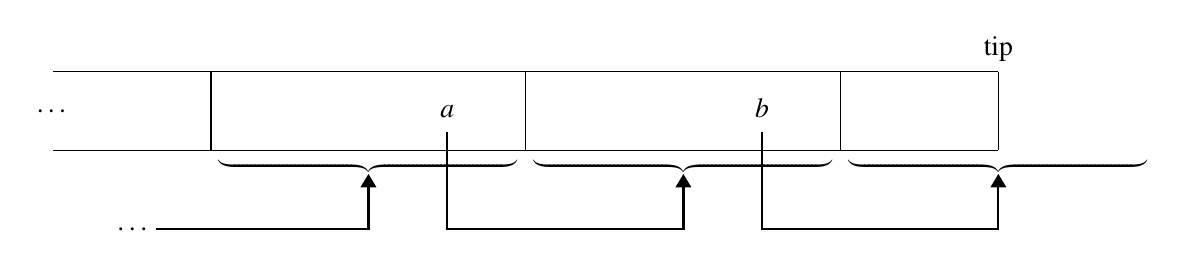
\begin{tikzpicture}
%                             /--------\
%                             |        |
%                             *        v  tip
% 1 -----+------------+------------+-----+
%        |       *    |            |     * current stake
% 0 -----+------------+------------+-----|
%   -10  -8           -4           0     2
%                |          ^
%                \----------/
\draw (-10, 0.5) node{\ldots};
\draw (-10,  0) --  (2, 0);
\draw (-10,  1) --  (2, 1);
\draw  (-8,  0) -- (-8, 1);
\draw  (-4,  0) -- (-4, 1);
\draw   (0,  0) --  (0, 1);
\draw   (2,  0) --  (2, 1) node[above]{tip};
\draw  (-6, -0.2) node {$\underbrace{\hspace{3.8cm}}$};
\draw  (-2, -0.2) node {$\underbrace{\hspace{3.8cm}}$};
\draw  ( 2, -0.2) node {$\underbrace{\hspace{3.8cm}}$};
\draw [thick, arrows={-Triangle}] (-9, -1) node[fill=white] {$\ldots$}-- (-6, -1) -- (-6, -0.3);
\draw [thick, arrows={-Triangle}] (-5, 0.5) node[fill=white] {$\mathstrut a$} -- (-5, -1) -- (-2, -1) -- (-2, -0.3);
\draw [thick, arrows={-Triangle}] (-1, 0.5) node[fill=white] {$\mathstrut b$} -- (-1, -1) -- (2, -1) -- (2, -0.3);
\end{tikzpicture}
\end{center}
%
This makes it possible to \emph{forecast} what the stake distribution (i.e.,
the ledger view) will be at various points. For example, if the chain looks like
%
\begin{center}
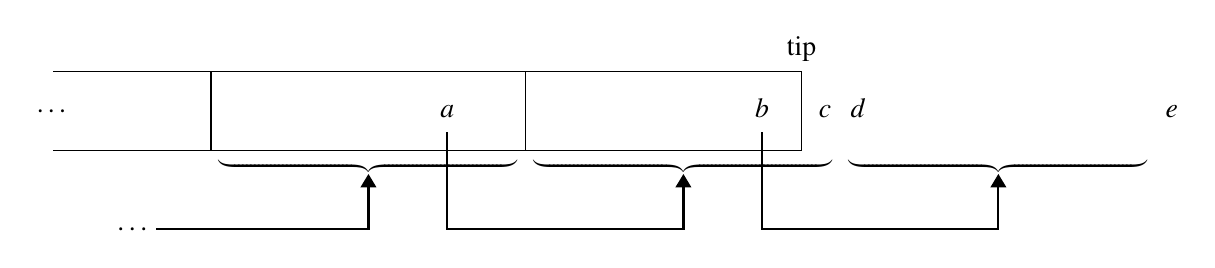
\begin{tikzpicture}
\draw (-10,    0.5) node{\ldots};
\draw (-10,    0) -- (-0.5, 0);
\draw (-10,    1) -- (-0.5, 1);
\draw  (-8,    0) -- (-8,   1);
\draw  (-4,    0) -- (-4,   1);
\draw  (-0.5,  0) -- (-0.5, 1) node[above]{tip};
\draw  (-6,   -0.2) node {$\underbrace{\hspace{3.8cm}}$};
\draw  (-2,   -0.2) node {$\underbrace{\hspace{3.8cm}}$};
\draw  ( 2,   -0.2) node {$\underbrace{\hspace{3.8cm}}$};
\draw [thick, arrows={-Triangle}] (-9, -1) node[fill=white] {$\ldots$}-- (-6, -1) -- (-6, -0.3);
\draw [thick, arrows={-Triangle}] (-5, 0.5) node[fill=white] {$\mathstrut a$} -- (-5, -1) -- (-2, -1) -- (-2, -0.3);
\draw [thick, arrows={-Triangle}] (-1, 0.5) node[fill=white] {$\mathstrut b$} -- (-1, -1) -- (2, -1) -- (2, -0.3);
\draw (0, 0.5) node[left] {$\mathstrut c$};
\draw (0, 0.5) node[right] {$\mathstrut d$};
\draw (4, 0.5) node[right] {$\mathstrut e$};
\end{tikzpicture}
\end{center}
%
then we can ``forecast'' that the stake distribution at point $c$ will be the one
established at point $a$, whereas the stake distribution at point $d$ will be the
one established at point $b$. The stake distribution at point $e$ is however not
yet known; we say that $e$ is ``out of the forecast range''.

\subsection{Code}

Since we're always forecasting what the ledger would look like \emph{if it would
be advanced to a particular slot}, the result of forecasting is always something
ticked:\footnote{Actually we never deal with an \emph{unticked} ledger view.}
%
\begin{lstlisting}
data Forecast a = Forecast {
      forecastAt  :: WithOrigin SlotNo
    , forecastFor :: SlotNo -> Except OutsideForecastRange (Ticked a)
    }
\end{lstlisting}
%
Here \lstinline!forecastAt! is the tip of the ledger in which the forecast was
constructed and \lstinline!forecastFor! is constructing the forecast for a
particular slot, possibly returning an error message of that slot is out of
range. This terminology---a forecast constructed \emph{at} a slot
and computed \emph{for} a slot---is used throughout both this technical report
as well as the consensus layer code base.

\subsection{Ledger view}
\label{forecast:ledgerview}

For the ledger view specifically, the \lstinline!LedgerSupportsProtocol!
class (\cref{ledger:api:LedgerSupportsProtocol}) requires a function
%
\begin{lstlisting}
ledgerViewForecastAt ::
     LedgerConfig blk
  -> LedgerState blk
  -> Forecast (LedgerView (BlockProtocol blk))
\end{lstlisting}
%
This function must satisfy two important properties:
%
\begin{description}
\item[Sufficient range]

When we validate headers from an upstream node, the most recent usable ledger
state we have is the ledger state at the intersection of our chain and the chain
of the upstream node. That intersection will be at most $k$ blocks back, because
that is our maximum rollback (\cref{consensus:overview:k}). Furthermore, it is
only useful to track an upstream peer if we might want to adopt their blocks,
and we only switch to their chain if it is longer than ours
(\cref{consensus:overview:chainsel}). This means that in the worst case
scenario, with the intersection $k$ blocks back, we need to be able to evaluate
$k + 1$ headers in order to adopt the alternative chain. However, the range of a
forecast is based on \emph{slots}, not blocks; since not every slot may contain
a block (\cref{time:slots-vs-blocks}), the range needs to be sufficient to
\emph{guarantee} to contain at least $k + 1$ blocks\footnote{Due to a
misalignment between the consensus requirements and the Shelley specification,
this is not the case for Shelley, where the effective maximum rollback is in
fact $k - 1$; see \cref{shelley:forecasting}).}; we will come back to this in
\cref{future:block-vs-slot}.

The network layer may have additional reasons for wanting a long forecast
range; see \cref{nonfunctional:network:headerbody}.

\item[Relation to ticking]
Forecasting is not the only way that we can get a ledger view for a particular
slot; alternatively, we can also \emph{tick} the ledger state, and then ask
for the ledger view at that ticked ledger state. These two ways should give us
the same answer:
%
\begin{equation}
\begin{array}{lllll}
\mathrm{whenever} &
\mathtt{forecastFor} \; (\mathtt{ledgerViewForecastAt}_\mathit{cfg} \; l) \; s & = & \mathtt{Right} & l' \\
\mathrm{then} & \mathtt{protocolLedgerView}_\mathit{cfg} \; (\mathtt{applyChainTick}_\mathit{cfg} \; s \; l) & = && l'
\end{array}
\end{equation}
%
In other words, whenever the ledger view for a particular slot is within the
forecast range, then ticking the ledger state to that slot and asking for the
ledger view at the tip should give the same answer. Unlike forecasting, however,
ticking has no maximum range. The reason is the following fundamental difference between these two concepts:
%
\begin{quote}
\textbf{(Forecast vs. ticking)} When we \emph{forecast} a ledger view, we are
predicting what that ledger view will be, \emph{no matter which blocks will  be
applied to the chain} between the current tip and the slot of the forecast. By
contrast, when we \emph{tick} a ledger, we are applying any time-related
changes to the ledger state in order to apply the \emph{next} block; in other
words, when we tick to a particular slot, \emph{there \emph{are} no blocks in
between the current tip and the slot we're ticking to}. Since there are no
intervening blocks, there is no uncertainty, and hence no limited range.
\end{quote}
\end{description}

\section{Queries}
\label{ledger:queries}

\section{Abandoned approach: historical states}

\chapter{Serialisation abstractions}
\label{serialisation}

Some of the various pieces of data that are handled by consensus also need to be
serialised to a binary format so that they can be:

\begin{enumerate}
\item written/read to/from \emph{storage} (see \cref{storage}) or;
\item sent/received across the \emph{network} (e.g., headers via the chain sync
  protocol \cref{chainsyncclient}).
\end{enumerate}

The two serialisation purposes above have different requirements and are
independent of each other. For example, when establishing a network connection,
a version number is negotiated. We can vary the network serialisation format
depending on the version number, allowing for instance to include some more
information in the payload. A concrete example of this is that starting from a
certain version, we include the block size in the payload when sending a
Byron\todo{Can I talk about Byron here?} header across the network as the header
itself does not contain it. This kind of versioning only concerns the network
and is independent of the storage layer. Hence we define separate abstractions
for them, decoupling them from each other.

For both abstractions, we use the CBOR (Concise Binary Object
Representation)\todo{command for acronyms?} format, because it has the following
benefits, paraphrasing the \texttt{cborg} library\todo{link?}:
\begin{itemize}
\item fast serialisation and deserialisation
\item compact binary format
\item stable format across platforms (32/64bit, big/little endian)
\item potential to read the serialised format from other languages
\item incremental or streaming (de)serialisation
\item suitable to use with untrusted input (resistance to asymmetric resource consumption attacks)
\item ...
\end{itemize}
Moreover, CBOR was chosen for the initial implementation of the Cardano
blockchain,\todo{correct?} with which we must maintain binary compatibility.
While it was possible to switch to another format for the block types developed
after the initial implementation, we saw no reason to switch.

We will now discuss both serialisation abstractions in more detail.

\section{Serialising for storage}
\label{serialisation:storage}

The following data is stored on disk (see \cref{storage}):

\begin{itemize}
\item Blocks
\item The extended ledger state (\cref{storage:extledgerstate}) which is the
  combination of:
  \begin{itemize}
  \item The header state (\cref{storage:headerstate})
  \item The ledger state\todo{link?}
  \end{itemize}
\end{itemize}

We use the following abstraction for serialising data to and from disk:

\begin{lstlisting}
class EncodeDisk blk a where
  encodeDisk :: CodecConfig blk -> a -> Encoding

class DecodeDisk blk a where
  decodeDisk :: CodecConfig blk -> forall s. Decoder s a
\end{lstlisting}

\begin{itemize}
\item These type classes have two type parameters: the block \lstinline!blk!,
  over which most things are parameterised, and \lstinline!a!, the type to
  (de)serialise. For example, \lstinline!a! can be the block type itself or the
  type corresponding to the ledger state.
\item \lstinline!CodecConfig blk! is a data family that defines the extra
  configuration needed for (de)serialisation. For example, to deserialise an EBB
  (\cref{ebbs}), the number of slots per epoch needs to be known statically to
  compute the slot of the block based on the epoch number, as the serialisation
  of an EBB does not contain its slot number, but the in-memory representation
  does. This configuration is kept as small as possible and is ideally empty.
\item The \lstinline!a -> Encoding! and \lstinline!forall s. Decoder s a! are
  the types for respectively encoders and decoders of the \lstinline!cborg!
  library.\todo{link?}
\item The encoder and decoder are split in two classes because they are not
  always \emph{symmetric}: the instantiation of \lstinline!a! in the encoder is
  not always the same as in the corresponding decoder. This is because blocks
  are \emph{annotated} with their serialisation. We discuss this in more detail
  in \cref{serialisation:annotations}.
\end{itemize}

\subsection{Nested contents}
\label{serialisation:storage:nested-contents}

By writing a block to disk we automatically have written the block's header to
disk, as the header is a part of the block. While we never write just a header,
we do support \emph{reading} just the header. This is more efficient than
reading the entire block and then extracting the header, as fewer bytes have to
be read from disk and deserialised.

\begin{center}
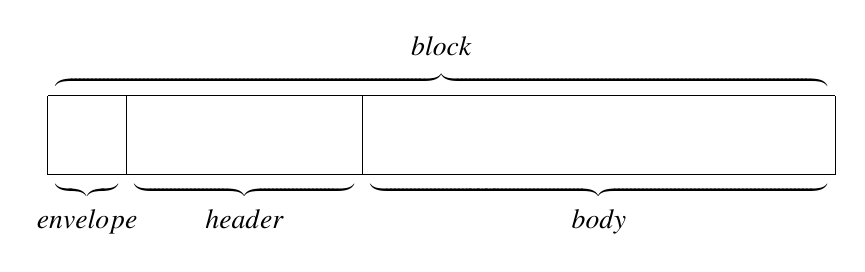
\begin{tikzpicture}
\draw  (0,    0)  -- (10,  0);
\draw  (0,    1)  -- (10,  1);
\draw  (0,    0)  --  (0,  1);
\draw  (1,    0)  --  (1,  1);
\draw  (4,    0)  --  (4,  1);
\draw (10,    0)  -- (10,  1);
\draw  (5,    1.2) node {$\overbrace{\hspace{9.8cm}}$};
\draw  (5,    1.6) node[fill=white] {$\mathstrut block$};
\draw  (0.5, -0.2) node {$\underbrace{\hspace{0.8cm}}$};
\draw  (0.5, -0.6) node[fill=white] {$\mathstrut envelope$};
\draw  (2.5, -0.2) node {$\underbrace{\hspace{2.8cm}}$};
\draw  (2.5, -0.6) node[fill=white] {$\mathstrut header$};
\draw  (7,   -0.2) node {$\underbrace{\hspace{5.8cm}}$};
\draw  (7,   -0.6) node[fill=white] {$\mathstrut body$};
\end{tikzpicture}
\end{center}

Extracting the header from a block on disk can be very simple, like in the
figure above. The block starts with an envelope, which is followed by the block
header and the block body. In this case, we read the bytes starting from the
start of the header until the end of the header, which we then decode. We use
the following abstraction to represent this information:

\begin{lstlisting}
data BinaryBlockInfo = BinaryBlockInfo {
      headerOffset :: !Word16
    , headerSize   :: !Word16
    }

class HasBinaryBlockInfo blk where
  getBinaryBlockInfo :: blk -> BinaryBlockInfo
\end{lstlisting}

As the size of a header can vary on a per-block basis, we maintain this
information \emph{per block} in the storage layer.\todo{link?} We trade four
extra bytes of storage and memory space for faster reading of headers.

However, it is not for every type of block the case that the encoding of a
header can literally be sliced out of the encoding of the corresponding block.
The serialisation of a header when embedded in a block might be different from
the serialisation of a header on its own. For example, the standalone header
might require an additional envelope or a different one than the block's
envelope.

A concrete example of this are the Byron blocks and headers. A Byron block is
either a regular block or an epoch boundary block (EBB) (discussed in
\cref{ebbs}). A regular block has a different header than an EBB, consequently,
their encoding differs. The envelope of the encoding of a Byron block includes a
tag indicating whether the block is a regular block or an EBB, so that the
decoder knows what kind of header and body to expect. For the same reason, the
envelope of the encoding of a standalone Byron header includes the same tag.
However, when we slice out the header from the Byron block and feed that to the
decoder for Byron headers, the envelope containing the tag will be
\emph{missing}.

The same problem presents itself for the hard fork combinator (\cref{hfc}): when
using the hard fork combinator to combine two block types, A and B, into one,
the block's envelope will (typically) indicate whether it is a block of type A
or B. The header corresponding to such a block will have a similar envelope.
When we slice the header out of such a block, the required envelope will be
missing. The right envelope has to be prepended so that the header decoder knows
whether it should expect A or B.

The header is \emph{nested} inside the block and to be able to decode it, we
need some more \emph{context}, i.e., the envelope of the header. In the storage
layer (\cref{storage}), we store the context of each block in an index
(in-memory or on-disk, depending on the database) so that after reading both the
context and the sliced header, we can decode the header without having to read
and decode the entire block. We capture this idea in the following abstractions.

\begin{lstlisting}
data family NestedCtxt_ blk :: (Type -> Type) -> (Type -> Type)
\end{lstlisting}
As usual, we parameterise over the block type. We also parameterise over another
functor, e.g., \lstinline!f!, which in practice will be instantiated to
\lstinline!Header!, but in the future, there might be more types of nested
contents, other than headers, e.g., block bodies. The constructors of this data
family will represent the different types of context available, e.g., for Byron
a context for regular blocks and a context for EBBs.

\lstinline!NestedCtxt! is indexed by \lstinline!blk!: it is the block that
determines this type. However, we often want to partially apply the second
argument (the functor), leaving the block type not yet defined, hence we define:
\begin{lstlisting}
newtype NestedCtxt f blk a = NestedCtxt {
      flipNestedCtxt :: NestedCtxt_ blk f a
    }
\end{lstlisting}
The \lstinline!a! type index will correspond to the raw, sliced header that
requires the additional context. It can vary with the context, e.g., the context
for a Byron EBB will fix \lstinline!a! to a raw EBB header (without the
necessary envelope).

Now that we have defined \lstinline!NestedCtxt!, we can define the class that
allows us to separate the nested type (the header) into the context and the raw,
sliced type (the raw header, \lstinline!a!), as well as the inverse:
\begin{lstlisting}
class (..) => HasNestedContent f blk where
  unnest :: f blk -> DepPair (NestedCtxt f blk)
  nest   :: DepPair (NestedCtxt f blk) -> f blk
\end{lstlisting}
\lstinline!DepPair! is a dependent pair that allows us to hide the type
parameter \lstinline!a!. When writing a block, \lstinline!unnest! is used to
extract the context so that it can be stored in the appropriate index. When
reading a header, \lstinline!nest! is used to combine the context, read from the
appropriate index, with the raw header into the header.

In certain scenarios, we do not have access to the separately stored context of
the block, but we do have access to the encoded block, in which case we should
be able to able to extract the context directly from the encoded block, without
having to decode it entirely. We use the \lstinline!ReconstructNestedCtxt! class
for this:
\begin{lstlisting}
class HasNestedContent f blk => ReconstructNestedCtxt f blk where
  reconstructPrefixLen  :: proxy (f blk) -> PrefixLen
  reconstructNestedCtxt ::
       proxy (f blk)
    -> ShortByteString
    -> ..
    -> SomeSecond (NestedCtxt f) blk
\end{lstlisting}
The \lstinline!PrefixLen! is the number of bytes extracted from the beginning of
the encoded block required to reconstruct the context. The
\lstinline!ShortByteString! corresponds to these bytes. The
\lstinline!reconstructNestedCtxt! method will parse this bytestring and return
the corresponding context. The \lstinline!SomeSecond! type is used to hide the
type parameter \lstinline!a!.

As these contexts and context-dependent types do not fit the mould of the
\lstinline!EncodeDisk! and \lstinline!DecodeDisk! classes described in
\cref{serialisation:storage}, we define variants of these classes:
\begin{lstlisting}
class EncodeDiskDepIx f blk where
  encodeDiskDepIx :: CodecConfig blk
                  -> SomeSecond f blk -> Encoding

class DecodeDiskDepIx f blk where
  decodeDiskDepIx :: CodecConfig blk
                  -> Decoder s (SomeSecond f blk)

class EncodeDiskDep f blk where
  encodeDiskDep :: CodecConfig blk -> f blk a
                -> a -> Encoding

class DecodeDiskDep f blk where
  decodeDiskDep :: CodecConfig blk -> f blk a
                -> forall s. Decoder s (ByteString -> a)
\end{lstlisting}
\todo{explain?}

\section{Serialising for network transmission}
\label{serialisation:network}

The following data is sent across the network:
\begin{itemize}
\item Header hashes
\item Blocks
\item Headers
\item Transactions
\item Transaction IDs
\item Transaction validation errors
\item Ledger queries
\item Ledger query results
\end{itemize}
\todo{less whitespace}

We use the following abstraction for serialising data to and from the network:

\begin{lstlisting}
class SerialiseNodeToNode blk a where
  encodeNodeToNode :: CodecConfig blk
                   -> BlockNodeToNodeVersion blk
                   -> a -> Encoding
  decodeNodeToNode :: CodecConfig blk
                   -> BlockNodeToNodeVersion blk
                   -> forall s. Decoder s a

class SerialiseNodeToClient blk a where
  encodeNodeToClient :: CodecConfig blk
                     -> BlockNodeToClientVersion blk
                     -> a -> Encoding
  decodeNodeToClient :: CodecConfig blk
                     -> BlockNodeToClientVersion blk
                     -> forall s. Decoder s a
\end{lstlisting}

These classes are similar to the ones used for storage
(\cref{serialisation:storage}), but there are some important differences:

\begin{itemize}
\item The encoders and decoders are always symmetric, which means we do not have
  to separate encoders from decoders and can merge them in a single class.
  Nevertheless, some of the types sent across the network still have to deal
  with annotations (\cref{serialisation:annotations}), we discuss how we solve
  this in \cref{serialisation:network:cbor-in-cbor}.
\item We have separate classes for \emph{node-to-node} and \emph{node-to-client}
  serialisation.\todo{link?}
  By separating them, we are more explicit about which data is serialised for
  which type of connection. Node-to-node protocols and node-to-client protocols
  have different properties and requirements. This also gives us the ability to,
  for example, use a different encoding for blocks for node-to-node protocols
  than for node-to-client protocols.
\item The methods in these classes all take a \emph{version} as argument. We
  will discuss versioning in \cref{serialisation:network:versioning}.
\end{itemize}

\subsection{Versioning}
\label{serialisation:network:versioning}

As requirements evolve, features are added, data types change, constructors are
added and removed. For example, adding the block size to the Byron headers,
adding new ledger query constructors, etc. This affects the data we send across
the network. In a distributed network of nodes, it is a given that not all nodes
will simultaneously upgrade to the latest released version and that nodes
running different versions of the software, i.e., different versions of the
consensus layer, will try to communicate with each other. They should of course
be able to communicate with each other, otherwise the different versions would
cause partitions in the network.

This means we should be careful to maintain binary compatibility between
versions. The network layer is faced with the same issue: as requirements
evolve, network protocols (block fetch, chain sync\todo{link?}) are modified
change (adding messages, removing messages, etc.), network protocols are added
or retired, etc. While the network layer is responsible for the network
protocols and the encoding of their messages, the consensus layer is responsible
for the encoding of the data embedded in these messages. Changes to either
should be possible without losing compatibility: a node should be able to
communicate successfully with other nodes that run a newer or older version of
the software, up to certain limits (old versions can be retired eventually).

To accomplish this, the network layer uses \emph{versions}, one for each bundle
of protocols:
\begin{lstlisting}
data NodeToNodeVersion
    = NodeToNodeV_1
    | NodeToNodeV_2
    | ..

data NodeToClientVersion
    = NodeToClientV_1
    | NodeToClientV_2
    | ..
\end{lstlisting}
For each backwards-incompatible change, either a change in the network protocols
or in the encoding of the consensus data types, a new version number is
introduced in the corresponding version data type. When the network layer
establishes a connection with another node or client, it will negotiate a
version number during the handshake: the highest version that both parties can
agree on. This version number is then passed to any client and server handlers,
which decide based on the version number which protocols to start and which
protocol messages (not) to send. A new protocol message would only be sent when
the version number is greater or equal than the one with which it was
introduced.

This same network version is passed to the consensus layer, so we can follow the
same approach. However, we decouple the network version numbers from the
consensus version numbers for the following reason. A new network version number
is needed for each backwards-incompatible change to the network protocols or the
encoding of the consensus data types. This is clearly a strict superset of the
changes caused by consensus. When the network layer introduces a new protocol
message, this does not necessarily mean anything changes in the encoding of the
consensus data types. This means multiple network versions can correspond to the
same consensus-side encoding or \emph{consensus version}. In the other
direction, each change to the consensus-side encodings should result in a new
network version. We capture this in the following abstraction:
\begin{lstlisting}
class (..) => HasNetworkProtocolVersion blk where
  type BlockNodeToNodeVersion   blk :: Type
  type BlockNodeToClientVersion blk :: Type

class HasNetworkProtocolVersion blk
   => SupportedNetworkProtocolVersion blk where
  supportedNodeToNodeVersions ::
       Proxy blk -> Map NodeToNodeVersion   (BlockNodeToNodeVersion   blk)
  supportedNodeToClientVersions ::
       Proxy blk -> Map NodeToClientVersion (BlockNodeToClientVersion blk)
\end{lstlisting}
The \lstinline!HasNetworkProtocolVersion! class has two associated types to
define the consensus version number types for the given block. When no
versioning is needed, one can use the unit type as the version number. The
\lstinline!SupportedNetworkProtocolVersion! defines the mapping between the
network and the consensus version numbers. Note that this does not have to be an
injection, as multiple network version can most certainly map to the same
consensus version. Nor does this have to be a surjection, as old network and
consensus versions might be removed from the mapping when the old version no
longer needs to be supported. This last reason is also why this mapping is
modelled with a \lstinline!Map! instead of a function: it allows enumerating a
subset of all defined versions, which is not possible with a function.

\todo{TODO} Global numbering vs multiple block types

The \lstinline!SerialiseNodeToNode! and \lstinline!SerialiseNodeToClient!
instances can then branch on the passed version to introduce changes to the
encoding format, for example, the inclusion of the block size in the Byron
header encoding.

Consider the following scenario: a change is made to one of the consensus data
types, for example, a new query constructor is added the ledger query data type.
This requires a new consensus and thus network version number, as older versions
will not be able to decode it. What should be done when the new query
constructor is sent to a node that does not support it (the negotiated version
is older than the one in which the constructor was added)? If it is encoded and
send, the receiving side will fail to decode it and terminate its
connection.\todo{right?} This is rather confusing to the sender, as they are
left in the dark. Instead, we let the \emph{encoder} throw an exception in this
case, terminating that connection, so that the sender is at least notified of
this. \todo{TODO} Ideally, we could statically prevent such cases.

\subsection{CBOR-in-CBOR}
\label{serialisation:network:cbor-in-cbor}

In \cref{serialisation:annotations}, we explain why the result of the decoder
for types using \emph{annotations} needs to be passed the original encoding as a
bytestring. When reading from disk, we already have the entire bytestring in
memory,\todo{explain why} so it can easily be passed to the result of the
decoder. However, this is not the case when receiving a message via the network
layer: the entire message, containing the annotated type(s), is decoded
incrementally.\todo{right?} When decoding CBOR, it is not possible to obtain the
bytestring corresponding to what the decoder is decoding. To work around this,
we use \emph{CBOR-in-CBOR}: we encode the original data as CBOR and then encode
the resulting bytestring as CBOR \emph{again}. When decoding CBOR-in-CBOR, after
decoding the outer CBOR layer, we have exactly the bytestring that we will need
for the annotation. Next, we feed this bytestring to the original decoder, and,
finally, we pass the bytestring to the function returned by the decoder.

\subsection{Serialised}
\label{serialisation:network:serialised}

One of the duties of the consensus layer is to serve blocks and headers to other
nodes in the network.\todo{link?} To serve for example a block, we read it from
disk, deserialise it, and then serialise it again and send it across the
network. The costly deserialisation and serialisation steps cancel each other
out and are thus redundant. We perform this optimisation in the following way.
When reading such a block from storage, we do not read the \lstinline!blk!, but
the \lstinline!Serialised blk!, which is a phantom type around a raw, still
serialised bytestring:
\begin{lstlisting}
newtype Serialised a = Serialised ByteString
\end{lstlisting}
To send this serialised block over the network, we have to encode this
\lstinline!Serialised blk!. As it happens, we use CBOR-in-CBOR to send both
blocks and headers over the network, as described in
\cref{serialisation:network:cbor-in-cbor}. This means the serialised block
corresponds to the inner CBOR layer and that we only have to encode the
bytestring again as CBOR, which is cheap.

This optimisation is only used to \emph{send} and thus encode blocks and
headers, not when \emph{receiving} them, because each received block or header
will have to be inspected and validated, and thus deserialised anyway.

As discussed in \cref{serialisation:storage:nested-contents}, reading a header
(nested in a block) from disk requires reading the context and the raw header,
and then combining them before we can deserialise the header. This means the
approach for serialised headers differs slightly:
\begin{lstlisting}
newtype SerialisedHeader blk = SerialisedHeaderFromDepPair {
      serialisedHeaderToDepPair :: GenDepPair Serialised
                                              (NestedCtxt Header blk)
    }
\end{lstlisting}
This is similar to the \lstinline!DepPair (NestedCtxt f blk)! type from
\cref{serialisation:storage:nested-contents}, but this time the raw header is
wrapped in \lstinline!Serialised! instead of being deserialised.

\section{Annotations}
\label{serialisation:annotations}

\todo{TODO} move up? The previous two sections refer to this

The following technique is used in the Byron and Shelley ledgers for a number of
data types like blocks, headers, transactions, \ldots The in-memory representation
of, for example a block, consists of both the typical fields describing the
block (header, transactions, \ldots), but also the \emph{serialisation} of the block
in question. The block is \emph{annotated} with its serialisation.

The principal reason for this is that it is possible that multiple
serialisations, each which a different hash, correspond to the same logical
block. For example, a client sending us the block might encode a number using a
binary type that is wider than necessary (e.g., encoding the number 0 using four
bytes instead of a single byte). CBOR defines a \emph{canonical format}, we call
an encoding that is in CBOR's canonical format a \emph{canonical
encoding}.\todo{link?}

When after deserialising a block in a non-canonical encoding, we serialise it
again, we will end up with a different encoding, i.e., the canonical encoding,
as we stick to the canonical format. This means the hash, which is part of the
blockchain, is now different and can no longer be verified.

For this reason, when deserialising a block, the original, possibly
non-canonical encoding is retained and used to annotate the block. To compute
the hash of the block, one can hash the annotated serialisation.

Besides solving the issue with non-canonical encodings, this has a performance
advantage, as encoding such a block is very cheap, it is just a matter of
copying the in-memory annotation.

\todo{TODO} We rely on it being cheap in a few places, mention that/them?

\todo{TODO} extra memory usage

This means that the result of the decoder must be passed the original encoding
as a bytestring to use as the annotation of the block or other type in question.
Hence the decoder corresponding to the encoder \lstinline!blk -> Encoding! has
type \lstinline!forall s. Decoder s (ByteString -> blk)!, which is a different
instantiation of the type \lstinline!a!, explaining the split of the
serialisation classes used for storage (\cref{serialisation:storage}). The
original encoding is then applied to the resulting function to obtain the
annotated block. This asymmetry is handled in a different way for the network
serialisation, namely using CBOR-in-CBOR
(\cref{serialisation:network:cbor-in-cbor}).

\subsection{Slicing}

\todo{TODO} discuss the slicing of annotations with an example. What is the
relation between the decoded bytestring and the bytestring passed to the
function the decoder returns? Talk about compositionality.


\part{Storage Layer}

\chapter{Overview}
\label{storage}

\section{Components}
\label{storage:components}

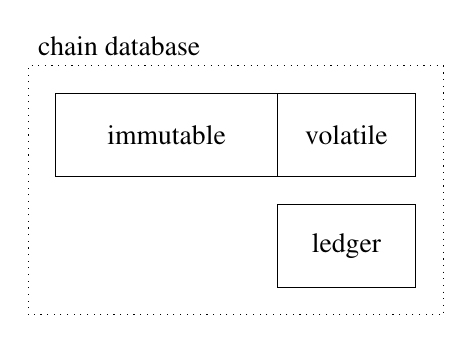
\begin{tikzpicture}
\draw [dotted]
     (-50pt, -65pt)
  -- ++(0, 90pt) node[above right] {chain database}
  -- ++(150pt, 0)
  -- ++(0, -90pt)
  -- cycle;
\node [draw, shape=rectangle, minimum width=80pt, minimum height=30pt] at (0,0)  {immutable};
\node [draw, shape=rectangle, minimum width=50pt, minimum height=30pt] at (65pt, 0)  {volatile};
\node [draw, shape=rectangle, minimum width=50pt, minimum height=30pt] at (65pt, - 40pt) {ledger};
\end{tikzpicture}

Discuss the immutable/volatile split (we reference this section for that).

\section{In memory}
\label{storage:inmemory}

TODO: After we discussed the overview, we should give an overview of everything
we store in memory in any component, so that we have a better understanding of
memory usage of the chain DB as a whole.

\subsection{Chain fragments}
\label{storage:fragments}

\subsection{Extended ledger state}
\label{storage:extledgerstate}
\label{storage:headerstate}

TODO: Is there a more natural place to talk about this? Introducing the
header state when introducing the storage layer does not feel quite right.
The storage layer might be storing the header state, but that doesn't
explain its existence.

ChainDepState, (ChainIndepState), LedgerState, ExtLedgerState

\chapter{Immutable Database}
\label{immutable}

\chapter{Volatile Database}
\label{volatile}

\chapter{Ledger Database}
\label{ledgerdb}

\section{Initialisation}
\label{ledgerdb:initialisation}

Describe why it is important that we store a single snapshot and then replay
ledger events to construct the ledger DB.

\newcommand{\chainle}{\ensuremath{\mathrel{\sqsubseteq}}}
\newcommand{\chainlt}{\ensuremath{\mathrel{\sqsubset}}}
\newcommand{\chainnotlt}{\ensuremath{\mathrel{\nsqsubset}}}
\newcommand{\wehave}{.\;}
\newcommand{\suchthat}{.\;}
\newcommand{\app}{\ensuremath{\mathrel{\triangleright}}}
\newcommand{\length}[1]{\ensuremath{\mathrm{length} \; #1}}
\newcommand{\ifthen}[2]{\ensuremath{\mathrm{if} \quad #1 \quad \mathrm{then} \quad #2}}
\renewcommand{\iff}{\ensuremath{\qquad\mathrm{iff}\qquad}}
\newcommand{\candidates}[2]{\ensuremath{\mathsf{candidates}_#1(#2)}}
\newcommand{\blockNo}[1]{\ensuremath{\mathtt{blockNo}(#1)}}
\newcommand{\selectviewle}{\ensuremath{\precsim}}

\chapter{Chain Selection}
\label{chainsel}

Chain selection is one of the central responsibilities of the chain database
(\cref{chaindb}). It of course depends on chain selection as it is defined  by
the consensus protocol (\cref{consensus:class:chainsel}), but needs to  take
care of a lot of operational concerns. In this chapter we will take a closer
look at the implementation of chain selection in the chain database, and state
some properties and sketch some proofs to motivate it.

\section{Comparing anchored fragments}
\label{chainsel:fragments}

\subsection{Introduction}

Recall from \cref{consensus:overview:chainsel} that while in the literature
chain selection is defined in terms of comparisons between entire chains, we
instead opted to model it in terms of a comparison between the \emph{headers} at
the tip of those chains (or rather, a \emph{view} on those headers defined by
the specific consensus protocol).

We saw in \cref{storage:inmemory} (specifically, \cref{storage:fragments}) that
the consensus layer stores chain fragments in memory (the most recent headers on
a chain), both for the node's own current chain as well as for upstream nodes
(which we refer to as ``candidate chains''). Defining chain selection in terms
of fragments is straight-forward when those fragments are non-empty: we simply
take the most recent header, extract the view required by the consensus protocol
(\cref{BlockSupportsProtocol}), and then use the consensus protocol's chain
selection interface to compare them. The question is, however, how to compare
two fragments when one (or both) of them is \emph{empty}. This problem is more
subtle than it might seem at first sight, and requires careful consideration.

We mentioned in \cref{consensus:overview:chainsel} that consensus imposes a
fundamental assumption that the strict extension of a chain is always (strictly)
preferred over that chain (\cref{prefer-extension}), and that consequently we
\emph{always} prefer a non-empty chain over an empty one (and conversely we
\emph{never} prefer an empty chain over a non-empty one). However, chain
fragments are mere proxies for their chains, and the fragment might be empty
even if the chain is not. This means that in principle it's possible we do not
prefer a non-empty fragment over an empty one, or indeed prefer an empty
fragment over a non-empty one. However, when a fragment is empty, we cannot rely
on the consensus protocol's chain selection because we have no header to give
it.

Let's consider under which conditions these fragments might be empty:

\begin{description}
\item[Our fragment]
Our own fragment is a path through the volatile database, anchored at the tip of
the immutable database (\cref{storage:fragments}). Under normal circumstances,
it will be empty only if our \emph{chain} is empty; we will refer to such empty
fragments as \emph{genuinely empty}.\footnote{We can distinguish between an empty
fragment of a non-empty chain and a (necessarily) empty fragment of an empty
chain by looking at the anchor point: if it is the genesis point, the chain must
be empty.} However, our fragment can also be empty even when our chain is not,
if due to data loss the volatile database is empty (or contains no blocks that
fit onto the tip of the immutable database).

\item[Candidate fragment]
A \emph{genuinely} empty candidate fragment, representing an empty candidate
chain, is never preferred over our chain. Unfortunately, however, the candidate
fragment as maintained by the chain sync client (\cref{chainsyncclient}) can
essentially be empty at any point due to the way that a switch-to-fork is
implemented in terms of rollback followed by roll forward: after a maximum
rollback (and before the roll forward), the candidate fragment is empty.
\end{description}

\subsection{Precondition}
\label{chainsel:fragments:precondition}

Since neither of these circumstances can be avoided, we must therefore impose a
precondition for chain selection between chain fragments to be definable:

\begin{definition}[Precondition for comparing chain fragments]
The two fragments must either both be non-empty, or they must intersect.
\end{definition}

In this chapter, we establish this precondition in two different ways:

\begin{enumerate}
\item When we construct candidates chains (potential chains that we may wish
to replace our own chain with), those candidate chains must intersect with
our own chain within $k$ blocks from its tip; after all, if that is not the
case, we would induce a roll back of more than $k$ blocks
(\cref{consensus:overview:k}).

\item When we compare fragments to each other, we only compare fragments from a
set of fragments that are all anchored at the same point (i.e., the anchor of
all fragments in the set is the same, though it might be different from the
anchor of our current fragment). Since they are all anchored at the same point,
they trivially all intersect with each other.
\end{enumerate}

There is one more use of fragment selection, which is rather more subtle;
we will come back to this in \cref{chainsyncclient:plausiblecandidates}.

\todo{TODO} TODO: Throughout we are talking about \emph{anchored} fragments
here. We should make sure that we discuss those somewhere.

\subsection{Definition}
\label{chainsel:fragments:definition}

We will now show that this precondition suffices to compare two fragments,
whether or not they are empty; we'll consider each case in turn.

\begin{description}

\item[Both fragments empty]
Since the two fragments must intersect, that intersection point can only
be the two anchor points, which must therefore be equal. This means that
two fragments represent the same chain: neither fragment is preferred
over the other.

\item[First fragment non-empty, second fragment empty]
Since the two fragments must intersect, that intersection can only be the
anchor of the second fragment, which can lie anywhere on the first fragment.

\begin{itemize}
\item If it lies at the \emph{tip} of the first fragment, the two fragments represent the
same chain, and neither is preferred over the other.
\item If it lies \emph{before} the tip of first fragment, the first fragment is
a strict extension of the second, and is therefore is preferred over the
second.
\end{itemize}

\item[First fragment empty, second fragment non-empty]
This case is entirely symmetric to the previous; if the intersection is the
tip of the second fragment, the fragments represent the same chain. Otherwise,
the second fragment is a strict extension of the first, and is therefore
preferred.

\item[Both fragments non-empty]
In this case, we can simply use the consensus protocol chain selection API
to compare the two most recent headers on both fragments.

\end{description}

Note that this relies critically on the ``prefer extension'' rule
(\cref{prefer-extension}).

\section{Preliminaries}
\label{chainsel:spec}

Recall from \cref{storage:components} that the immutable database stores a
linear chain, terminating in the \emph{tip} $I$ of the immutable database. The
volatile database stores a (possibly fragmented) tree of extensions to that
chain:
%
\begin{center}
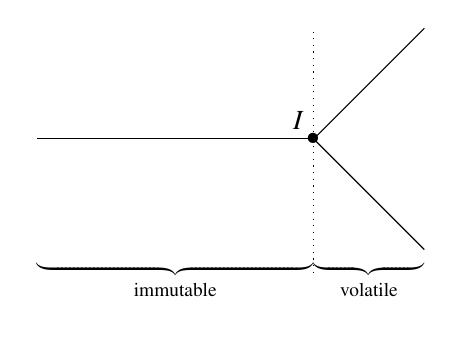
\begin{tikzpicture}
\draw (0,0) -- (100pt, 0) coordinate (immtip) node{$\bullet$} node[above left] {$I$};
\draw (immtip) -- ++(40pt,  40pt);
\draw (immtip) -- ++(40pt, -40pt);
\draw [dotted] (immtip) -- ++(0, 40pt);
\draw [dotted] (immtip) -- ++(0, -50pt);
\node at (50pt, -40pt) [below] {$\underbrace{\hspace{100pt}}_\textrm{immutable}$};
\node at (120pt, -40pt) [below] {$\underbrace{\hspace{40pt}}_\textrm{volatile}$};
\end{tikzpicture}
\end{center}
%
The node's \emph{current chain} is stored in memory as a chain fragment through
the volatile database, anchored at $I$.  When we start up the node, the chain
database must find the best possible path through the volatile database and
adopt that as our current fragment; every time a new block is added to the
volatile database, we have to recompute the new best possible path. In other
words, we maintain the following invariant:

\begin{definition}[Current chain invariant]
\label{current-chain-invariant}
The current chain is the best possible path through the volatile DB.
\end{definition}

``Best'' of course is according to the chain selection rule defined by the
consensus protocol (\cref{consensus:class:chainsel}). In this section we
describe how the chain database establishes and preserves this invariant.

\subsection{Notation}

So far we have been relatively informal in our description of chain selection,
but in order to precisely describe the algorithm and state some of its
properties, we have to introduce some notation.

\begin{definition}[Chain selection]
We will model chain selection as a transitive binary relation (\chainlt) between
valid chains (it is undefined for invalid chains), and let $C \chainle C'$ if
and only if $C \chainlt C'$ or $C = C'$. It follows that (\chainle) is a partial
order (reflexive, antisymmetric, and transitive).
\end{definition}

For example, the simple ``prefer longest chain'' chain selection rule could be
given as
%
\begin{equation*}
\tag{longest chain rule}
C \chainlt C'  \iff  \length{C} < \length{C'}
\end{equation*}

In general of course the exact rule depends on the choice of consensus protocol.
\Cref{prefer-extension} (\cref{consensus:overview:chainsel}) can now be
rephrased as
%
\begin{equation}
\label{eq:prefer-extension}
\forall C, B \wehave C \chainlt (C \app B)
\end{equation}

We will not be comparing whole chains, but rather chain fragments
(we will leave the anchor of fragments implicit):
%
\begin{definition}[Fragment selection]
We lift $\chainlt$ to chain fragments in the manner described in
\cref{chainsel:fragments}; this means that $\chainlt$ is undefined for two
fragments if they do not intersect (\cref{chainsel:fragments:precondition}).
\end{definition}

We also lift $\chainle$ to \emph{sets} of fragments, intuitively indicating that
a particular fragment is the ``best choice'' out of a set $\mathcal{S}$ of
candidate fragments:
%
\begin{definition}[Optimal candidate]
\begin{equation*}
\mathcal{S} \chainle F  \iff   \nexists F' \in \mathcal{S} \suchthat F \chainlt F'
\end{equation*}
(in other words, if additionally $F \in \mathcal{S}$, then $F$ is a maximal
element of $C$). This inherits all the preconditions of $\chainle$ on chains and
fragments.
\end{definition}

Finally, we will introduce some notation for \emph{computing} candidate
fragments:\footnote{In order to compute these candidates efficiently, the
volatile database must support a ``forward chain index'', able to efficiently
answer the question ``which blocks succeed this one?''.}

\begin{definition}[Construct set of candidates]
Given some set of blocks $V$, and some anchor $A$ (with $A$ either a block or
the genesis point), $$\candidates{A}{V}$$ is the set of chain fragments
anchored at $A$ using blocks picked from $V$.
\end{definition}

By construction all fragments in $\candidates{A}{V}$ have the same anchor, and
hence all intersect (at $A$); this will be important for the use of the
$\chainle$ operator.

\subsection{Properties}

\begin{lemma}[Properties of the set of candidates]
\label{candidates:properties}
The set of candidates computed by $\candidates{A}{V}$ has the following
properties.

\begin{enumerate}

\item \label{candidates:prefixclosed}
It is prefix closed:
\begin{equation*}
\forall F, B \wehave
\ifthen
  {(F \app B) \in \candidates{A}{V}}
  {F \in \candidates{A}{V}}
\end{equation*}

\item \label{candidates:appendnew}
If we add a new block into the set, we can append that block to existing
candidates (where it fits):
\begin{equation*}
\ifthen
  {F \in \candidates{A}{V}}
  {F \app B \in \candidates{A}{V \cup \{ B \}}}
\end{equation*}
provided $F$ can be extended with $B$.

\item \label{candidates:monotone}
Adding blocks doesn't remove any candidates:
\begin{equation*}
\candidates{A}{V} \subseteq \candidates{A}{V \cup \{B\}}
\end{equation*}

\item \label{candidates:musthavenew}
If we add a new block, then any new candidates must involve that new block:
\begin{equation*}
\ifthen
  {F \in \candidates{A}{V \cup \{B\}}}
  {F \in \candidates{A}{V} \text{ or } F = (\ldots \app B \app \ldots)}
\end{equation*}

\end{enumerate}
\end{lemma}

The next lemma says that if we have previously found some optimal candidate $F$,
and subsequently learn of a new block $B$, it suffices to find a locally optimal
candidate \emph{amongst the candidates that involve $B$}; this new candidate
will also be a globally optimal candidate.

\begin{lemma}[Focus on new block]
\label{focusonnewblock}
Suppose we have $F, F_\mathit{new}$ such that
\begin{enumerate}
\item \label{focusonnewblock:previouslyoptimal}
$\candidates{A}{V} \chainle F$
\item \label{focusonnewblock:optimalamongstnew}
$(\candidates{A}{V \cup \{B\}} \setminus \candidates{A}{V}) \chainle F_\mathit{new}$
\item \label{focusonnewblock:betterthanold}
$F \chainle F_\mathit{new}$
\end{enumerate}
Then
\begin{equation*}
\candidates{A}{V \cup \{B\}} \chainle F_\mathit{new}
\end{equation*}
\end{lemma}

\begin{proof}
Suppose there exists $F' \in \candidates{A}{V \cup \{B\}}$ such that
$F_\mathit{new} \chainlt F'$. By transitivity and
assumption~\ref{focusonnewblock:betterthanold}, $F \chainlt F'$. As
shown in \cref{candidates:properties} (\cref{candidates:musthavenew}), there are two possibilities:

\begin{itemize}
\item $F' \in \candidates{A}{V}$, which would violate
assumption~\cref{focusonnewblock:previouslyoptimal}, or
\item $F'$ must contain block $B$, which would violate
assumption~\cref{focusonnewblock:optimalamongstnew}.
\end{itemize}
\end{proof}

\section{Initialisation}
\label{chainsel:init}

The initialisation of the chain database proceeds as follows.

\begin{enumerate}

\item
\label{chaindb:init:imm}
Initialise the immutable database, determine its tip $I$, and ask the
ledger DB for the corresponding ledger state $L$.

\item Compute the set of candidates anchored at the immutable database's tip
\label{chaindb:init:compute}
$I$ using blocks from the volatile database $V$
$$\candidates{I}{V}$$
ignoring known-to-be-invalid blocks (if any; see \cref{chaindb:invalidblocks})
and order them using $(\chainlt)$  so that we process better candidates
first.\footnote{Technically speaking we should \emph{first} validate all
candidates, and only then apply selection to the valid chains. We perform chain
selection first, because that is much cheaper. Both approaches are semantically
equivalent, since \lstinline!sortBy f . filter p = filter p . sortBy f! due to
the stability of \lstinline!sortBy!.} Candidates that are strict prefixes of
other candidates can be ignored (as justified by the ``prefer extension''
assumption, \cref{prefer-extension}).\footnote{The implementation does not
compute candidates, but rather ``maximal'' candidates, which do not include such
prefixes.}

\item
\label{chaindb:init:select}
Not all of these candidates may be valid, because the volatile database stores
blocks whose \emph{headers} have been validated, but whose \emph{bodies} are
still unverified (other than to check that they correspond to their headers).
We therefore validate each candidate chain fragment, starting with $L$ (the
ledger state at the tip of the immutable database) each time.\footnote{We make
no attempt to share ledger states between candidates, even if they share a
common prefix, trading runtime performance for lower memory pressure.}

As soon as we find a candidate that is valid, we adopt it as our current chain.
If we find a candidate that is \emph{invalid}, we mark the invalid
block\footnote{There is no need to mark any successors of invalid blocks; see
\cref{chaindb:dont-mark-invalid-successors}.} (unless it is invalid due to
potential clock skew, see \cref{chainsel:infuture}), and go back to
step~\ref{chaindb:init:compute}. It is important to recompute the set of
candidates after marking some blocks as invalid because those blocks may also
exist in other candidates and we do not know how the valid prefixes of those
candidates should now be ordered.

\end{enumerate}

\section{Adding new blocks}
\label{chainsel:addblock}

When a new block $B$ is added to the chain database, we need to add it to the
volatile DB and recompute our current chain. We distinguish between the
following different cases.

Before we process the new block, we first run chain selection on any blocks that
had previously been temporarily shelved because their slot number was (just)
ahead of the wallclock (\cref{chainsel:infuture}). We do this independent of what
we do with the new block.\footnote{In a way, calls to \lstinline!addBlock! are
how the chain database sees time advance. It does not rely on slot length to do
so, because slot length is ledger state dependent.}

The implementation \lstinline!addBlock! additionally provides  client code with
various notifications throughout the process  (``block added'', ``chain
selection run'', etc.). We will not describe these notifications here.

\subsection{Ignore}

We can just ignore the block if any of the following is true.

\begin{itemize}

\item
The block is already in the immutable DB, \emph{or} it belongs to a branch which
forks more than $k$ blocks away from our tip, i.e.\footnote{The check is a
little more complicated in the presence of EBBs (\cref{ebbs}). This is relevant
if we switch to an alternative fork after a maximum rollback, and that
alternative fork starts with an EBB. It is also relevant when due to data
corruption the volatile database is empty and the first block we add when we
continue to sync the chain happens to be an EBB.}
%
\begin{equation*}
\blockNo{B} \leq \blockNo{I}
\end{equation*}
%
We could distinguish between between the block being on our chain or on a
distant fork by doing a single query on the immutable database, but it does not
matter: either way we do not care about this block.

We don't expect the chain sync client to feed us such blocks under normal
circumstances, though it's not impossible: by the time a block is downloaded
it's conceivable, albeit unlikely, that that block is now older than $k$.

\item
The block was already in the volatile database, i.e.
%
\begin{equation*}
B \in V
\end{equation*}

\item
The block is known to be invalid (\cref{chaindb:invalidblocks}).

\end{itemize}

\subsection{Add to current chain}
\label{chainsel:addtochain}

If $B$ fits onto the end of our current fragment $F$ (and hence onto our current chain) $F$, i.e.
%
\begin{itemize}
\item $F$ is empty, and $B_\mathit{pred} = I$
(where $I$ must necessarily also be the anchor of the fragment), or
\item $\exists F' \suchthat F = F' \app B_\mathit{pred}$
\end{itemize}
%
then any new candidates must be equal to or an extension of $F \app B$
(\cref{candidates:properties}, \cref{candidates:musthavenew}); this set is
computed by
%
\begin{equation*}
(F \app B \app \candidates{B}{V \cup \{B\}})
\end{equation*}
%
Since all candidates would be strictly preferred over $F$ (since they are
extensions of $F$), by \cref{focusonnewblock} it suffices to pick the best
candidate amongst these extensions. Apart from the starting point, chain
selection then proceeds in the same way as when we are initialising the database
(\cref{chainsel:init}).

This case takes care of the common case where we just add a block to our chain,
as well as the case where we stay with the same branch but receive some blocks
out of order. Moreover, we can use the \emph{current} ledger state as the
starting point for validation.

\subsection{Store, but don't change current chain}

When we are missing one of the (transitive) predecessors of the block, we store
the block but do nothing else. We can check this by following back pointers
until we reach a block $B'$ such that $B' \notin V$ and $B' \neq I$. The cost of
this is bounded by the length of the longest fragment in the volatile DB, and
will typically be low; moreover, the chain fragment we are constructing this way
will be used in the switch-to-fork case
(\cref{chainsel:switchtofork}).\footnote{The function that constructs these
fragments is called \lstinline!isReachable!.}

At this point we \emph{could} do a single query on the immutable DB to check if
$B'$ is in the immutable DB or not. If it is, then this block is on a distant
branch that we will never switch to, and so we can ignore it. If it is not, we
may or may not need this block later and we must store it; if it turns out we
will never need it, it will eventually be garbage collected (\cref{chaindb:gc}).

An alternative and easier approach is to omit the check on the immutable DB,
simply assuming we might need the block, and rely on garbage collection to
eventually remove it if we don't. This is the approach we currently use.

\subsection{Switch to a fork}
\label{chainsel:switchtofork}

If none of the cases above apply, we have a block $B$ such that

\begin{enumerate}
\item \label{chainsel:switchtofork:notinvoldb}
$B \notin V$
\item \label{chainsel:switchtofork:notinimmdb}
$\blockNo{B} > \blockNo{I}$ (and hence $B$ cannot be in the immutable DB)
\item \label{chainsel:switchtofork:connected}
For all transitive predecessors $B'$ of $B$ we have $B' \in V$ or $B' = I$.
In other words, we must have a fragment
$$F_\mathit{prefix} = I \app \ldots \app B$$
in $\candidates{I}{V \cup \{B\}}$.
\item \label{chainsel:switchtofork:doesnotfit}
(Either $F$ is empty and $B_\mathit{pred} \neq I$, or) $\exists F', B' \suchthat
F = F' \app B'$ where $B' \neq B_\mathit{pred}$; i.e., block does not fit onto
current chain.\footnote{\Cref{chainsel:switchtofork:connected} rules out the
first option: if $B_\mathit{pred} \neq I$ then we must have $B_\mathit{pred} \in
V$ and moreover this must form some kind of chain back to $I$; this means that
the preferred candidate cannot be empty.}
\end{enumerate}

We proceed in similar fashion to the case when the block fit onto the tip of our
chain (\cref{chainsel:addtochain}). The new candidates in $\candidates{I}{V \cup
\{B\}}$ must involve $B$ (\cref{candidates:properties},
\cref{candidates:musthavenew}), which in this case means they must all be
extensions of $F_\mathit{prefix}$; we can compute these candidates
using\footnote{The implementation of the chain database actually does not
construct fragments that go back to $I$, but rather to the intersection point
with the current chain. This can be considered to be an optimisation of what we
describe here.}
$$I \app \ldots \app B \app \candidates{B}{V \cup \{B\}}$$
Not all of these fragments might be preferred over the current chain; we filter
those out.\footnote{Recall that the current chain gets special treatment: when
two candidates are equally preferable, we can pick either one, but when a
candidate and the current chain are equally preferable, we must stick with the
current chain.} We then proceed as usual, considering each of the remaining
fragments in $(\chainle)$ order, and appeal to \cref{focusonnewblock}
again to conclude that the fragment we find in this way will be an optimal
candidate across the entire volatile database.


%
% *
%
% *
%
%
% It is worth pointing out that we do _not_ rely on `F_prefix` being longer than
% the current chain. Indeed, it may not be: if two leaders are selected for the
% same slot, and we _receive_ a block for the current slot before we can _produce_
% one, our current chain will contain the block from the other leader; when we
% then produce our own block, we end up in the switch-to-fork case; here it is
% important that `preferCandidate` would prefer a candidate chain (the chain that
% contains our own block) over our current chain, even if they are of the same
% length, if the candidate ends in a block that we produced (and the current chain
% does not); however, the `ChainDB` itself does not need to worry about this
% special case.
%
% [let's be explicit about the difference between current chain and self
% produced blocks]
%

\section{In-future check}
\label{chainsel:infuture}

As we saw in \cref{chainsel:spec}, the chain DB performs full
block validation during chain selection. When we have validated a block, we then
do one additional check, and verify that the block's slot number is not ahead of
the wallclock time (for a detailed discussion of why we require the block's
ledger state for this, see \cref{time}, especially
\cref{time:block-infuture-check}). If the block is far ahead of the wallclock,
we treat this as any other validation error and mark the block as invalid.

Marking a block as invalid will cause the network layer to disconnect from the
peer that provided the block to us, since non-malicious (and non-faulty) peers
should never send invalid blocks to us. It is however possible that an upstream
peer's clock is not perfectly aligned with us, and so they might produce a block
which \emph{we} think is ahead of the wallclock but \emph{they} do not. To avoid
regarding such peers as malicious, the chain database supports a configurable
\emph{permissible clock skew}: blocks that are ahead of the wallclock by an
amount less than this permissible clock skew are not marked as invalid, but
neither will chain selection adopt them; instead, they simply remain in the
volatile database available for the next chain selection.

It is constructive to consider what happens if \emph{our} clock is off, in
particular, when it is slow. In this scenario \emph{every} (or almost every)
block that the node receives will be considered to be in the future. Suppose we
receive two consecutive blocks $A$ and $B$. When we receive $A$, chain selection
runs, we find that $A$ is ahead of the clock but within the permissible clock
skew, and we don't adopt it. When we then receive $B$, chain selection runs
again, we now discover the $A, B$ extension to our current chain; during
validation we cut off this chain at $B$ because it is ahead of the clock, but we
adopt $A$ because it is now valid.  In other words, we are always behind one
block, adopting each block only when we receive the \emph{next} block.

\begin{bug}
One problem with this scheme is that if we receive a block $B$ which is ahead of
the clock when we receive it, we might never notice it if block $B$ is not (yet)
connected to our chain: by the time we receive the missing blocks (which connect
$B$ to our chain), $B$ might no longer be ahead of the clock and we might adopt
it, even if $B$ was ahead by more than the permissible clock skew.

We could avoid this problem if we stored the time we received a block alongside
the block in the volatile database, but in the current design, the volatile
database does not store \emph{any} information on disk apart from raw blocks,
so this would be quite a significant design change.
\end{bug}

\section{Sorting}

In this chapter we have modelled chain selection as a partial order
$(\chainle)$. This suffices for the formal treatment, and in theory also
suffices for the implementation. However, at various points during the chain
selection process we need to \emph{sort} candidates in order of preference. We
can of course sort values based on a preorder only (topological sorting), but we
can do slightly better. Recall from \cref{consensus:class:chainsel} that we
require that the \lstinline!SelectView! on headers must be a total order. We can
therefore define

\begin{definition}[Same select view]
Let $C \selectviewle C'$ if the select view at the tip of $C$ is less than
or equal to the select view at the tip of $C'$.
\end{definition}

(\selectviewle) forms a total preorder (though not a partial order); if $C
\selectviewle C'$ \emph{and} $C' \selectviewle C$ then the select views at the
tips of $C$ and $C'$ are equal (though they might be different chains, of
course). Since $C \selectviewle C'$ implies $C' \chainnotlt C$, we can use this
preorder  to sort candidates (in order words, we will sort them \emph{on} their
select view, in Haskell-parlance).

\chapter{Chain Database}
\label{chaindb}

TODO\todo{TODO}: This is currently a disjoint collection of snippets.

\section{Block processing queue}
\label{chaindb:queue}

Discuss the chain DB's block processing queue, the future/promises/events,
concurrency concerns, etc.

Discuss the problem of the effective queue size (\#2721).

\section{Marking invalid blocks}
\label{chaindb:invalidblocks}

The chain database keeps a set of hashes of known-to-be-invalid blocks.
This information is used by the chain sync client (\cref{chainsyncclient}) to
terminate connections to nodes with a chain that contains an invalid block.

\begin{lemma}
\label{chaindb:dont-mark-invalid-successors}
When the chain database discovers an invalid block $X$, it is sufficient
to mark only $X$; there is no need to additionally mark any successors of $X$.
\end{lemma}

\begin{proof}[Proof (sketch).]
The chain sync client maintains a chain fragment corresponding to some suffix
of the upstream node's chain, and it preserves an invariant that that suffix
must intersect with the node's own current chain. It can therefore never be
the case that the fragment contains a successor of $X$ but not $X$ itself:
since $X$ is invalid, the node will never adopt it, and so a fragment that
intersects the node's current chain and includes a successor of $X$ \emph{must}
also contain $X$.
\end{proof}

TODO\todo{TODO}: We should discuss how this relates to GC (\cref{chaindb:gc}).

\section{Effective maximum rollback}

The maximum rollback we can support is bound by the length of the current  fragment. This will be less than $k$ only if

\begin{itemize}
\item We are near genesis and the immutable database is empty, or
\item Due to data corruption the volatile database lost some blocks
\end{itemize}

Only the latter case is some cause for concern: we are in a state where
conceptually we \emph{could} roll back up to $k$ blocks, but due to how we chose
to organise the data on disk (the immutable/volatile split) we cannot. One
option here would be to move blocks \emph{back} from the immutable DB to the
volatile DB under these circumstances, and indeed, if there were other parts of
the system where rollback might be instigated that would be the right thing to
do: those other parts of the system should not be aware of particulars of the
disk layout.

However, since the chain database is \emph{exclusively} in charge of switching
to forks, all the logic can be isolated to the chain database. So, when we have
a short volatile fragment, we will just not roll back more than the length of
that fragment. Conceptually this can be justified also: the fact that $I$ is the
tip of the immutable DB means that \emph{at some point} it was in our chain at
least $k$ blocks back, and so we considered it to be immutable: the fact that
some data loss occurred does not really change that. We may still roll back more
than $k$ blocks when disk corruption occurs in the immutable database, of
course.

One use case of the current fragment merits a closer examination. When the chain
sync client (\cref{chainsyncclient}) looks for an intersection between our chain
and the chain of the upstream peer, it sends points from our chain fragment. If
the volatile fragment is shorter than $k$ due to data corruption, the client
would have fewer points to send to the upstream node. However, this is the
correct behaviour: it would mean we cannot connect to upstream nodes who fork
more than $k$ of what \emph{used to be} our tip before the data corruption, even
if that's not where our tip is anymore. In the extreme case, if the volatile
database gets entirely erased, only a single point is available (the tip of the
immutable database $I$), and hence we can only connect to upstream nodes that
have $I$ on their chain.  This is precisely stating that we can only sync with
upstream nodes that have a chain that extends our immutable chain.

\section{Garbage collection}
\label{chaindb:gc}

Blocks on chains that are never selected, or indeed blocks whose
predecessor we never learn, will eventually be garbage collected when their
slot number number is more than $k$ away from the tip of the selected chain.\footnote{This is slot based rather than block based for historical
reasons only; we should probably change this.}

\begin{bug}
The chain DB (more specifically, the volatile DB) can still grow without bound
if we allow upstream nodes to rapidly switch between forks; this should be
addressed at the network layer (for instance, by introducing rate limiting for
rollback in the chain sync client, \cref{chainsyncclient}).
\end{bug}

Although this is GC of the volatile DB, I feel it belongs here more than in
the volatile DB chapter because here we know \emph{when} we could GC.
But perhaps it should be split into two: a section on how GC is implemented
in the volatile DB chapter, and then a section here how it's used in the
chain DB. References from elsewhere in the report to GC should probably
refer here, though, not to the vol DB chapter.

\subsection{GC delay}

For performance reasons neither the immutable DB nor the volatile DB ever makes
explicit \lstinline!fsync! calls to flush data to disk. This means that when the
node crashes, recently added blocks may be lost. When this happens in the
volatile DB it's not a huge deal: when the node starts back up and the chain
database is initialised we just run chain selection on whatever blocks still
remain; in typical cases we just end up with a slightly shorter chain.

However, when this happens in the immutable database the impact may be larger.
In particular, if we delete blocks from the volatile database as soon as we add
them to the immutable database, then data loss in the immutable database would
result in a gap between the volatile database and the immutable database, making
\emph{all} blocks in the volatile database unusable. We can recover from this, but it
would result in a large rollback (in particular, one larger than $k$).

To avoid this, we currently have a delay between adding blocks to the immutable
DB and removing them from the volatile DB (garbage collection). The delay is
configurable, but should be set in such a way that the possibility that the
block has not yet been written to disk at the time of garbage collection is
minimised;a a relatively short delay should suffice (currently we use a delay of
1 minute), though there are other reasons for preferring a longer delay:

\begin{itemize}
\item Clock changes can more easily be accommodated with more overlap (\cref{{future:clockchanges}})
\item The time delay also determines the worst-case validity of iterators
(todo\todo{TODO}: reference to relevant section).
\end{itemize}

Larger delays will of course result in more overlap between the two databases.
During normal node operation this might not be much, but the overlap might be
more significant during bulk syncing.

Notwithstanding the above discussion, an argument could be made that the
additional complexity due to the delay is not worth it; even a ``rollback'' of
more than $k$ is easily recovered from\footnote{Note that the node will never
actually notice such a rollback; the node would crash when discovering data
loss, and then restart with a smaller chain}, and clock changes as well, as
iterators asking for blocks that now live on distant chains, are not important
use cases. We could therefore decide to remove it altogether.

\chapter{Mempool}
\label{mempool}

\section{Consistency}
\label{mempool:consistency}

Discuss that we insist on \emph{linear consistency}, and why.


\part{Mini protocols}

\chapter{Chain sync client}
\label{chainsyncclient}

\section{Header validation}
\label{chainsyncclient:validation}

Discuss the fact that we validate headers (maybe a forward reference to the genesis chapter, where this becomes critical).

Discuss that this means we need efficient access to the $k$ most recent ledger states (we refer to this section for that).

\section{Forecasting requirements}
\label{chainsyncclient:forecasting}

Discuss that forecasting must have sufficient range to validate a chain longer than our own chain, so that we can meaningfully apply chain selection.

NOTE: Currently \cref{low-density} contains such a discussion.

\section{Trimming}
\label{chainsyncclient:trimming}

\section{Interface to the block fetch logic}
\label{chainsyncclient:plausiblecandidates}

We should discuss here the (very subtle!) reasoning about how we establish
the precondition that allows us to compare candidates
(\cref{chainsel:fragments:precondition}). See
\lstinline!plausibleCandidateChain! in \lstinline!NodeKernel!
(PR \#2735).

\chapter{Mini protocol servers}
\label{servers}

The division of work between the network layer and the consensus layer when it
comes to the implementation of the clients and servers of the mini protocols is
somewhat pragmatic. Servers and clients that do significant amounts of network
layer logic (such as block fetch client which is making delta-Q related
decisions, node-to-node transaction server and client, which are dealing with
transaction windows, etc), live in the network layer. Clients and servers that
primarily deal with consensus side concerns live in the consensus layer; the
chain sync client (\cref{chainsyncclient}), is the primary example of this.
There are also a number of servers for the mini protocols that do little more
than provide glue code between the mini protocol and the consensus interface;
these servers are described in this chapter.

\section{Local state query}
\label{servers:lsq}

\section{Chain sync}
\label{servers:chainsync}

\section{Local transaction submission}
\label{servers:txsubmission}

Unlike remote (node to node) transaction submission, local (client to node)
transaction submission does not deal with transaction windows, and is
consequently much simpler; it therefore lives consensus side rather than
network side.

\section{Block fetch}
\label{servers:blockfetch}


\part{Hard Fork Combinator}

\chapter{Overview}
\label{storage}

\section{Components}
\label{storage:components}

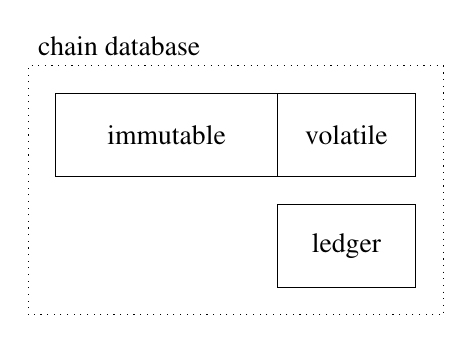
\begin{tikzpicture}
\draw [dotted]
     (-50pt, -65pt)
  -- ++(0, 90pt) node[above right] {chain database}
  -- ++(150pt, 0)
  -- ++(0, -90pt)
  -- cycle;
\node [draw, shape=rectangle, minimum width=80pt, minimum height=30pt] at (0,0)  {immutable};
\node [draw, shape=rectangle, minimum width=50pt, minimum height=30pt] at (65pt, 0)  {volatile};
\node [draw, shape=rectangle, minimum width=50pt, minimum height=30pt] at (65pt, - 40pt) {ledger};
\end{tikzpicture}

Discuss the immutable/volatile split (we reference this section for that).

\section{In memory}
\label{storage:inmemory}

TODO: After we discussed the overview, we should give an overview of everything
we store in memory in any component, so that we have a better understanding of
memory usage of the chain DB as a whole.

\subsection{Chain fragments}
\label{storage:fragments}

\subsection{Extended ledger state}
\label{storage:extledgerstate}
\label{storage:headerstate}

TODO: Is there a more natural place to talk about this? Introducing the
header state when introducing the storage layer does not feel quite right.
The storage layer might be storing the header state, but that doesn't
explain its existence.

ChainDepState, (ChainIndepState), LedgerState, ExtLedgerState

\newcommand{\timeconv}[2]{\ensuremath{\mathtt{Conv}_{#1}(#2)}}
\newcommand{\applyBlocks}[2]{\ensuremath{\mathtt{apply}_\mathit{#1}(#2)}}
\newcommand{\ledgertip}[1]{\ensuremath{\mathtt{tip}(#1)}}
\newcommand{\switch}[3]{\ensuremath{\mathtt{switch}_{(\mathit{#1},\;\mathit{#2})}(#3)}}

\chapter{Time}
\label{time}

\section{Introduction}
\label{time:introduction}

A fundamental property of the Ouroboros family of consensus protocols is that
they all divide time into discrete chunks called \emph{slots}; typically the
duration of a slot is on the order of seconds. In most Ouroboros protocols slots
are grouped into \emph{epochs}, with certain changes to the consensus chain
state happening at various points in an epoch. All nodes running the blockchain
agree on a \emph{system start time} (as a UTC time) through the chain's genesis
configuration, making the translation from a particular wallclock time to a slot
number easy: subtract the system start time from the wall clock time, and
divide by the slot length. This assumption that the mapping between wall clock
and slot or epoch numbers is always available permeated the consensus layer.
Unfortunately, it is not a valid assumption in the presence of hard forks.

It's not difficult to illustrate this with an example. Suppose we want to know
which slot time $t$ corresponds to in:
%
\begin{center}
\begin{tikzpicture}
\draw (0,0) -- (330pt, 0);
\draw [dotted] (180pt,20pt) node[above] {era transition} -- (180pt,-30pt);
\node at (273 pt,0) {$\bullet$};
\node at (273 pt,0) [above] {$t$};
% era 1
% slot length 6
% epoch size 10
% 3 epochs
\foreach \x in {0, 6, ..., 180} {
  \draw (\x pt, 0) -- +(0, -3pt);
}
\foreach \x in {0, 60, ..., 180} {
  \draw (\x pt, 0) -- +(0, -10pt);
}
% era 2
% slot length 3
% epoch size 16
% 3+ epochs
\foreach \x in {180, 183, ..., 330} {
  \draw (\x pt, 0) -- +(0, -3pt);
}
\foreach \x in {180, 228, ..., 330} {
  \draw (\x pt, 0) -- +(0, -10pt);
}
\end{tikzpicture}
\end{center}
%
We can read off from this depiction that $t$ is in epoch 1 \emph{of the second
era}, and relative slot 14 within that epoch. Since there are 16 slots to an
epoch in that era, that makes it slot $1 \times 16 + 14 = 30$ within that era.
The second era was preceded by three epochs in the first era, each of which
contained 10 slots, which means that time $t$ was slot $3 \times 10 + 30 = 60$
globally.

But now consider how this calculation changes if the era transition would have
happened one epoch later:
%
\begin{center}
\begin{tikzpicture}
\draw (0,0) -- (330pt, 0);
\draw [dotted] (240pt,20pt) node[above] {era transition} -- (240pt,-30pt);
\node at (273 pt,0) {$\bullet$};
\node at (273 pt,0) [above] {$t$};
% era 1
% slot length 6
% epoch size 10
% 4 epochs
\foreach \x in {0, 6, ..., 240} {
  \draw (\x pt, 0) -- +(0, -3pt);
}
\foreach \x in {0, 60, ..., 240} {
  \draw (\x pt, 0) -- +(0, -10pt);
}
% era 2
% slot length 3
% epoch size 16
% 1+ epochs
\foreach \x in {240, 243, ..., 330} {
  \draw (\x pt, 0) -- +(0, -3pt);
}
\foreach \x in {240, 288, ..., 330} {
  \draw (\x pt, 0) -- +(0, -10pt);
}
\node at (273 pt,0) {$\bullet$};
\node at (273 pt,0) [above] {$t$};
\end{tikzpicture}
\end{center}
%
Slot $t$ is now in epoch 0 of the second era, with relative
slot 11, making it slot $0 \times 16 + 11 = 11$ within the second era.
Since the second era got preceded by \emph{four} epochs of the first era,
that makes time $t$ global slot $4 \times 10 + 11 = 51$.

All of this would be no more than a minor complication if the exact moment of
the era transition would be statically known. This however is not the case: the
moment of the era transition is decided \emph{on the chain itself}. This leads
to the inevitable conclusion that time/slot conversions depend on the ledger
state, and may indeed be impossible: the slot at time $t$ is \emph{simply not
yet known} if the transition to era 2 has not been decided yet.

\section{Slots, blocks and stability}
\label{time:slots-vs-blocks}

In \cref{consensus:overview:k} we discussed the fundamental parameter $k$:
blocks that are more than $k$ blocks away from the tip of the chain are
considered to be immutable by the consensus layer and no longer subject to
rollback. We say that such blocks are \emph{stable}.

The ledger layer itself also depends on stability; for example, in Shelley the
stake distribution to be used for the leadership check needs to be stable before
it is adopted (this avoids malicious nodes from inspecting the leadership
schedule and then trying to cause a rollback if that leadership schedule is not
beneficial to them).

The ledger layer however does not use block numbers to determine stability, but
uses slot numbers to approximate it instead. This ultimately comes from the fact
that in Ouroboros the length of an \emph{epoch} is based on slots, not blocks,
although this is something we may wish to revisit (\cref{future:block-vs-slot}).

Depending on the particular choice of consensus algorithm, not all slots contain
blocks. For example, in Praos only a relatively small percentage of slots
contain blocks, depending on the Praos $f$ parameter (in Shelley, $f$ is set to
5\%). However,  the various Ouroboros protocols come with proofs (actually, a
probabilistic argument) providing a window of a certain number of slots that is
guaranteed to contain at least $k$ blocks; for example, for Ouroboros Classic
that window is $2k$ slots\footnote{Without much justification, we adopt this
same window for PBFT as well. It is almost certainly a gross overestimation.},
and for Ouroboros Praos that window is $3k/f$. Stability requirements in the
ledger then take the form ``at least $3k/f$ slots must have passed'' instead of
``at least $k$ blocks must have been applied''.

\section{Definitions}

\subsection{Time conversion}

As we saw in \cref{time:introduction}, we cannot do time conversions independent
of a ledger state. This motivates the following definition:

\begin{definition}[Time conversion]
Let $\timeconv{\sigma}{t}$ be the function that converts time $t$, with $t$
either specified as a wallclock time, a slot number, or an epoch number, to a
triplet
\begin{center}
(wallclock time, slot number, epoch number)
\end{center}
if $\sigma$ contains sufficient information to do so; $\timeconv{\sigma}{t}$
is undefined otherwise.
\end{definition}

Since all past era transitions are (obviously) known, time conversion should
always be possible for points in the past:

\begin{property}[Conversion for past points]
$\timeconv{\sigma}{t}$ should be defined for all $t \le \ledgertip{\sigma}$.
\end{property}

Furthermore, we assume that time conversion is monotone:

\begin{property}[Monotonicity of time conversion]
\label{time-conversion-monotone}
If $\timeconv{\sigma}{t}$ is defined, then $\timeconv{\applyBlocks{bs}{\sigma}}{t}$ must be as well and
\begin{equation*}
\timeconv{\applyBlocks{bs}{\sigma}}{t} = \timeconv{\sigma}{t}
\end{equation*}
\end{property}

\subsection{Forecast range}

Under certain conditions a ledger state may be usable to do time conversions
for slots ahead of the ledger state.

\begin{definition}[Forecast range]
We say that time $t > \ledgertip{\sigma}$ is within the forecast range of
$\sigma$ if \timeconv{\sigma}{t} is defined.
\end{definition}

Note that monotonicity (\cref{time-conversion-monotone}) should still
apply.

\subsection{Safe zone}

In order to be able to have a non-empty forecast range, we need to restrict
when era transitions can occur.

\begin{definition}[Safe zone]
A \emph{safe zone} is a period of time ahead of a ledger's tip in which an
era transition is guaranteed not to occur if it is not yet known.
\end{definition}

Intuitively, a non-empty safe zone means that there will be time between an
era transition being announced and it happening, no matter how the chain
is extended (no matter which blocks are applied):
%
\begin{equation}
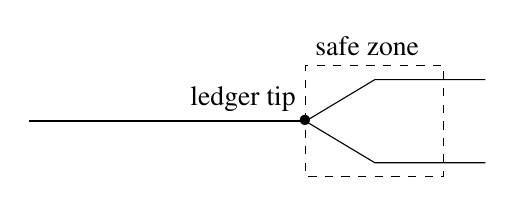
\begin{tikzpicture}[baseline=0pt]
\draw [thick] (-50pt,0) -- (50pt, 0) coordinate (tip);
\draw (tip) -- ++(25pt,  15pt) -- ++(40pt, 0pt);
\draw (tip) -- ++(25pt, -15pt) -- ++(40pt, 0pt);
\node at (tip) {$\bullet$};
\node at (tip) [above left] {ledger tip};
\draw [dashed] (tip)
            -- ++(0pt, 20pt) node[above right] {safe zone}
            -- ++(50pt, 0pt) -- ++(0pt, -40pt) -- ++(-50pt, 0pt) -- cycle;
\end{tikzpicture}
\end{equation}

\section{Ledger restrictions}
\label{time:ledgerrestrictions}

\subsection{Era transitions must be stable}

Monotonicity (\cref{time-conversion-monotone}) only talks about a chain's linear
history; since the consensus layer needs to deal with rollbacks (switching to
alternative chains) too, we will actually need a stronger property. Clearly,
time conversions cannot be invariant under switching to arbitrary chains; after
all, alternative chains might have era transitions in different places. The
consensus layer however does not \emph{support} switching to arbitrary
alternative chains; we have a maximum rollback (\cref{consensus:overview:k}),
and we never switch to a shorter chain (\cref{consensus:overview:chainsel},
\cref{never-shrink}). This means that we can model switching to an alternative
chain as $$\switch{n}{bs}{\sigma}$$ where $n \le k$ indicates how many blocks we
want to rollback, $\mathit{bs}$ is a list of new blocks we want to apply, and
$\mathtt{length} \; \mathit{bs} \ge n$.

\begin{property}[Time conversions stable under chain evolution]
\label{time-stable-under-evolution}
If \timeconv{\sigma}{t} is defined, then so is
\timeconv{\switch{n}{bs}{\sigma}}{t}
and moreover
\begin{equation*}
  \timeconv{\sigma}{t}
= \timeconv{\switch{n}{bs}{\sigma}}{t}
\end{equation*}
\end{property}

Intuitively, \cref{time-stable-under-evolution} says that we might not be able
to do time conversion for some time $t$ because it's outside our current forecast
range, but \emph{if} it is within forecast range, then we don't need to earmark
the answers we get from conversion as ``subject to rollback'': either we don't
know, or we know for sure. This requirement may not be strictly \emph{required}
for consensus to operate (\cref{future:relax-time-requirements}), but it is
a useful assumption which simplifies reasoning about time both within consensus
and within clients of the consensus layer such as the wallet.

The existence of safe zones is not sufficient to establish this stronger
property, in two ways:

\begin{itemize}
\item If we switch from a chain where an era transition is already known but
far in the future, to a chain on which the era transition happens much sooner
(or indeed, to a chain on which the era transition is not yet known), then
the forecast range will shrink and hence
\timeconv{\switch{n}{bs}{\sigma}}{t}
might not be defined, even if \timeconv{\sigma}{t} is.
\item Conversely, if we switch from a chain on which the era transition is
happening relatively soon, to a chain on which the era transition is happening
later, then the forecast range will not shrink, but the time conversions on
both chains will not agree with each other.\footnote{Going from a
chain on which the era transition is not yet known to one in which it \emph{is}
known is not problematic, due to safe zones.}
\end{itemize}

The key problem is that switching to an alternative chain can change our
information about future era transitions, and hence result in different time
conversions. We therefore insist that an era transition is not considered
``known'' until the block confirming the era transition is stable (no longer
subject to rollback). This means that the minimum distance from the announcement
of the era transition to the actual era transition must be $k$ plus the width of
the safe zone:
%
\begin{equation}
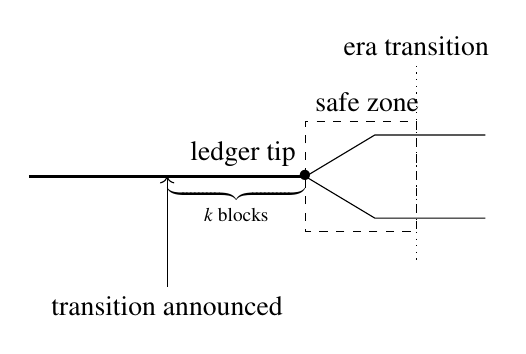
\begin{tikzpicture}[baseline=0pt]
\draw [thick] (-50pt,0) -- (50pt, 0) coordinate (tip);
\draw (tip) -- ++(25pt,  15pt) -- ++(40pt, 0pt);
\draw (tip) -- ++(25pt, -15pt) -- ++(40pt, 0pt);
\node at (tip) {$\bullet$};
\node at (tip) [above left] {ledger tip};
\draw [dashed] (tip)
            -- ++(0pt, 20pt) node[above right] {safe zone}
            -- ++(40pt, 0pt) coordinate (transition)
            -- ++(0pt, -40pt) -- ++(-40pt, 0pt) -- cycle;
\draw [dotted] (transition) ++(0pt, 20pt) node[above] {era transition}
            -- ++(0pt, -70pt);
\draw [<-] (tip) ++(-50pt, 0)
        -- +(0,-40pt) node[below] {transition announced};
% again, cheating...
\node at (25pt, -10pt) {$\underbrace{\hspace{50pt}}_\textrm{$k$ blocks}$};
\end{tikzpicture}
\end{equation}
%
Many ledgers set the width of the safe zone such that it guarantees at least $k$
blocks, but \emph{in principle} there is no need for the width of the safe zone
to be related to $k$ at all, although other parts of consensus might have
requirements for the width of the safe zone; we will discuss that in the next
section (\cref{time:ledgerrestrictions:safezones}).

\subsection{Size of the safezones}
\label{time:ledgerrestrictions:safezones}

The most important example of where we might need to do time translation for
blocks ahead of the ledger's tip is forecasting the Shelley ledger view
(\cref{ledger:forecasting}). The Shelley ledger view contains an abstraction
called \lstinline!EpochInfo! allowing the ledger to do time conversions, for
example to decide when rewards should be allocated.

As discussed in \cref{forecast:ledgerview}, it is important that the forecast
range of the ledger to allow us to validate at least $k + 1$ blocks after the
ledger tip; consequently, the safe zone of the ledger must be wide enough to
guarantee that it can span $k + 1$ blocks. This combination of the requirements
of the ledger with the header/body split
(\cref{nonfunctional:network:headerbody}) means that in practice the width of
the safe zone should be at least equal to the forecast range of the ledger, and
hence defined in terms of $k$ after all.

\subsection{Stability should not be approximated}

We discussed in \cref{time:slots-vs-blocks} that the ledger uses uses slot
numbers to approximate stability. Such an approximation would violate
\cref{time-stable-under-evolution}, however. Although we never switch to a
shorter chain in terms of blocks, it is certainly possible that we might switch
to a chain with a smaller \emph{slot} number at its tip: this would happen
whenever we switch to a longer but denser chain. If stability would be based on
slot numbers, this might mean that we could go from a situation in which the era
transition is considered known (and hence the forecast extends into the next
era) to a situation in which the era transition is not yet considered known (and
hence the forecast range only includes the safe zone in the current era).

Admittedly such a reduction of the forecast range would be temporary, and once
the era transition is considered known again, it will be in the same location;
after all, the block that confirmed the era transition \emph{is} stable. This
means that any previously executed time conversions would remain to be valid;
however, the fact that the forecast range shrinks might lead to unexpected
surprises. Using blocks rather than slot numbers to determine stability avoids
this problem.

\section{Properties}

\subsection{Forecast ranges arising from safe zones}

Slot length and epoch size can only change at era transitions. This means that
if the transition to the next era is not yet known, any time $t$ within the
era's safe zone is guaranteed to be within the era's forecast range. If the
transition to the next era \emph{is} known, the safe zone of the current era is
not relevant, but the safe zone of the next era is:
%
\begin{equation}
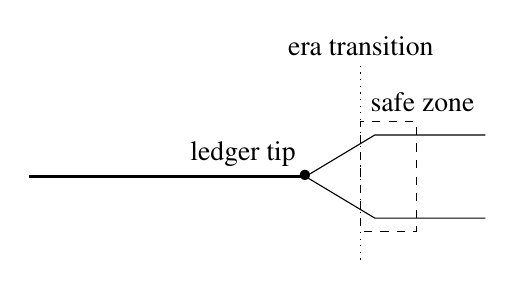
\begin{tikzpicture}[baseline=0pt]
\draw [thick] (-50pt,0) -- (50pt, 0) coordinate (tip);
\draw (tip) -- ++(25pt,  15pt) -- ++(40pt, 0pt);
\draw (tip) -- ++(25pt, -15pt) -- ++(40pt, 0pt);
\node at (tip) {$\bullet$};
\node at (tip) [above left] {ledger tip};
\draw [dashed] (tip) ++(20pt, 0pt) coordinate (transition)
            -- ++(0pt, 20pt) node[above right] {safe zone}
            -- ++(20pt, 0pt) -- ++(0pt, -40pt) -- ++(-20pt, 0pt) -- cycle;
\draw [dotted] (transition) ++(0pt, 40pt) node[above] {era transition}
            -- ++(0pt, -70pt);
\end{tikzpicture}
\end{equation}
%
The safe zone of the next era might be smaller or larger than (or indeed of
equal size as) the safe zone of the previous era; in this example it happens to
be smaller.

\Cref{hfc:era-transition-becoming-known} shows how the forecast range changes as
the next era transition becomes known; as shown, the next era starts at the
earliest possible moment (right after the safe zone); in general it could start
later than that, but of course not earlier (that would violate the definition of
the safe zone).

\begin{figure}

\begin{equation}
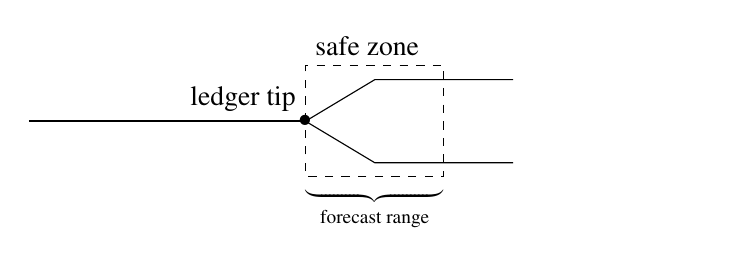
\begin{tikzpicture}[baseline=0pt]
\path (0,0) -- ++(200pt, 0pt); % adjust bounding box
\draw [thick] (-50pt,0) -- (50pt, 0) coordinate (tip);
\draw (tip) -- ++(25pt,  15pt) -- ++(50pt, 0pt);
\draw (tip) -- ++(25pt, -15pt) -- ++(50pt, 0pt);
\node at (tip) {$\bullet$};
\node at (tip) [above left] {ledger tip};
\draw [dashed] (tip)
            -- ++(0pt, 20pt) node[above right] {safe zone}
            -- ++(50pt, 0pt)
            -- ++(0pt, -40pt)
            -- ++(-50pt, 0pt) coordinate[pos=0.5] (safezone)
            -- cycle;
\node at (safezone) [below] {$\underbrace{\hspace{50pt}}_\textrm{forecast range}$};
\end{tikzpicture}
\end{equation}

\begin{equation}
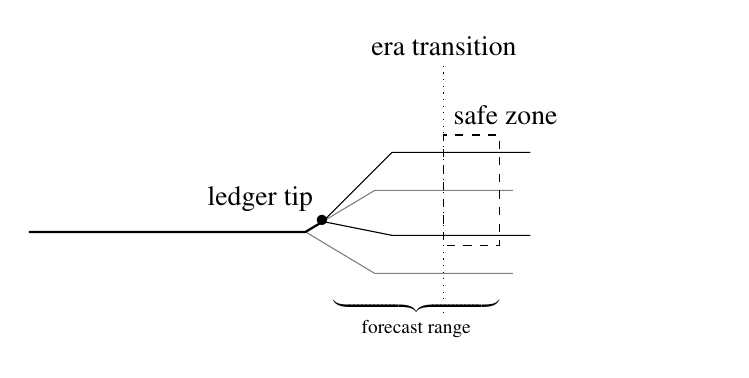
\begin{tikzpicture}[baseline=0pt]
\path (0,0) -- ++(200pt, 0pt); % adjust bounding box
\draw [gray] (-50pt,0) -- (50pt, 0) coordinate (oldtip);
\draw [gray, name path=chaintop] (oldtip) -- ++(25pt, 15pt) coordinate[pos=0.25] (tip) -- ++(50pt, 0pt);
\draw [gray] (oldtip) -- ++(25pt, -15pt) -- ++(50pt, 0pt);
\draw [thick] (-50pt,0) -- (50pt, 0) -- (tip);
\node at (tip) {$\bullet$};
\node at (tip) [above left] {ledger tip};
\draw (tip) -- ++(25pt, 25pt) -- +(50pt, 0pt);
\draw (tip) -- ++(25pt, -5pt) -- +(50pt, 0pt);
\draw [dotted, name path=transition]
        (oldtip) ++(50pt, 60pt) node[above] {era transition}
              -- ++(0pt, -90pt);
\path [name intersections={of=transition and chaintop}]
        (intersection-1) coordinate (safezone);
\draw [dashed] (safezone)
            -- ++(0pt, 20pt) node[above right] {safe zone}
            -- ++(20pt, 0pt)
            -- ++(0pt, -40pt)
            -- ++(-20pt, 0pt) coordinate[pos=0.5] (safezone)
            -- cycle;

% cheat: we should compute this of course :)
\node at (90pt,-20pt) [below] {$\underbrace{\hspace{60pt}}_\textrm{forecast range}$};
\end{tikzpicture}
\label{forecast-range-known-era-transition}
\end{equation}
\caption{\label{hfc:era-transition-becoming-known}Era transition becoming known}
\end{figure}

\subsection{Cross-fork conversions}
\label{time:cross-fork}

\begin{lemma}[Cross fork conversions]
Suppose we have the ledger state at some point $P$, and want to do time
conversions for time $t$ of a point $Q$ on a different fork of the chain:

\begin{center}
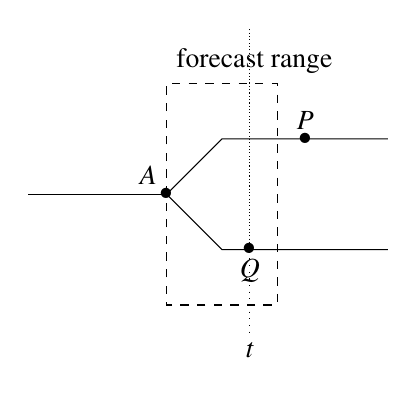
\begin{tikzpicture}
\draw (0,0) -- (50pt, 0) coordinate (A);
\draw (A) -- ++(20pt, 20pt)
          -- ++(30pt, 0) coordinate(P)
          -- ++(30pt, 0);
\draw (A) -- ++(20pt, -20pt)
          -- ++(10pt, 0) coordinate(Q1)
          -- ++(40pt, 0) coordinate(Q2)
          -- ++(10pt, 0);
\node at (A) {$\bullet$};
\node at (A) [above left] {$A$};
\node at (P) {$\bullet$};
\node at (P) [above] {$P$};
\node at (Q1) {$\bullet$};
\node at (Q1) [below] {$Q$};
\draw [dashed] (A) -- ++(0, 40pt) node[above right] {forecast range}
                   -- ++(40pt, 0)
                   -- ++(0, -80pt)
                   -- ++(-40pt, 0)
                   -- cycle;
\draw [dotted] (Q1) -- +(0, 80pt) -- +(0, -30pt) node[below] {$t$};
\end{tikzpicture}
\end{center}

Provided that $Q$ is within the forecast range of the common ancestor $A$
of $P$ and $Q$, the ledger state at $P$ can be used to do time conversions
for point $t$.
\end{lemma}

\begin{proof}
Since $t$ is within the forecast range at $A$, by definition $\timeconv{A}{t}$
is defined. By monotonicity (\cref{time-conversion-monotone}) we must have
\begin{align*}
\timeconv{A}{t} & = \timeconv{P}{t} \\
\timeconv{A}{t} & = \timeconv{Q}{t}
\end{align*}
It follows that $\timeconv{P}{t} = \timeconv{Q}{t}$.
\end{proof}

\section{Avoiding time}
\label{hfc:avoiding-time}

Time is complicated, and time conversions were pervasive throughout the
consensus layer. Despite the exposition above and the increased understanding,
we nonetheless have attempted to limit the use of time as much as possible,
in an attempt to simplify reasoning whenever possible. The use of
time within the core consensus layer is now very limited indeed:

\begin{enumerate}
\item When we check if we are a slot leader and need to produce a block, we
need to know the current time as a slot number (\todo{TODO.}We should discuss
this somewhere. The chapter on the consensus protocol discusses the protocol
side of things, but not the actual ``fork block production'' logic.)
\item When we add new blocks to the chain DB, we need to check if their slot
number is ahead of the wallclock (\cref{chainsel:infuture}).
\item Specific consensus protocols may need to do time conversions; for example,
Praos needs to know when various points in an epoch have been reached in order
to update nonces, switch stake distribution, etc.
\end{enumerate}

None of these use cases require either forecasting or cross-chain conversions.
The most important example of where forecasting is required is in projecting
the ledger view, as discussed in \cref{time:ledgerrestrictions:safezones}.
Cross-fork conversions (\cref{time:cross-fork}) may arise for example when the consensus layer makes time conversions available to tooling such as the wallet,
which may use it for example to show the wallclock of slots of blocks that may
not necessarily live on the current chain.

Keeping track of era transitions, and providing time conversions that take
them into account, is the responsibility of the hard fork combinator and
we will discuss it in more detail in \cref{hfc:time}.

In the remainder of this section we will discuss some simplifications
that reduced the reliance on time within the consensus layer.

\subsection{``Header in future'' check}
\label{time:header-infuture-check}

Recall from \cref{nonfunctional:network:headerbody} that block downloading
proceeds in two steps: first, the chain sync client downloads the block header
and validates it; if it finds that the header is valid, the block download logic
may decide to also download the block body, depending on chain selection
(\cref{consensus:overview:chainsel,consensus:class:chainsel}).

Suppose the node's own ledger state is at point $P$, and the incoming header is
at point $Q$. In order to validate the header, we need a ledger \emph{view} at
point $Q$ without having the ledger \emph{state} at point $Q$; this means that
point $Q$ must be within the ledger's forecast range at the common ancestor $A$
of $P$ and $Q$ (\cref{,ledger:forecasting}):

\begin{center}
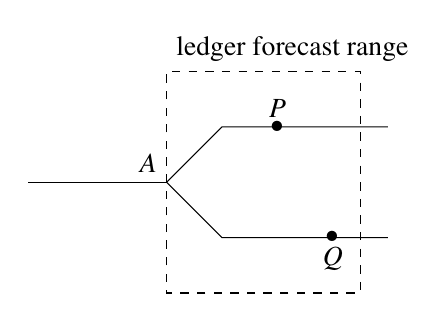
\begin{tikzpicture}
\draw (0, 0) -- (50pt, 0) coordinate (A);
\draw (A) -- ++(20pt,  20pt) -- ++(20pt, 0) coordinate (P) -- ++(40pt, 0);
\draw (A) -- ++(20pt, -20pt) -- ++(40pt, 0) coordinate (Q) -- ++(20pt, 0);
\node at (P) {$\bullet$};
\node at (Q) {$\bullet$};
\node at (A) [above left] {$A$};
\node at (P) [above] {$P$};
\node at (Q) [below] {$Q$};
\draw [dashed] (A) -- ++(0, 40pt) node[above right] {ledger forecast range}
                   -- ++(70pt, 0)
                   -- ++(0, -80pt)
                   -- ++(-70pt, 0)
                   -- cycle;
\end{tikzpicture}
\end{center}

As we have seen in \cref{time:cross-fork}, if $Q$ is within the \emph{time}
forecast range at $A$---put another way, if the time forecast range is at least
as wide as the ledger forecast range---then we also can use the ledger state at
$P$ to do time conversions at point $Q$. Moreover, as we saw in
\cref{time:ledgerrestrictions:safezones}, for many ledgers that inclusion
\emph{must} hold. If we make this a requirement for \emph{all} ledgers, in
principle the chain sync client could do a header-in-future check.

For simplicity, however, we nonetheless omit the check. As we will see in the
next section, the chain database must repeat this check \emph{anyway}, and so
doing it ahead of time in the chain sync client does not help very much;
skipping it avoids one more use of time within the consensus layer. Indeed, a
case could be made that we could skip header validation altogether, which would
alleviate the need for forecasting \emph{at all}; we will come back to this in
\cref{future:eliminating-forecasting}.

\subsection{Ahead-of-time ``block in future'' check}
\label{time:block-infuture-check}

In the original design of the chain database, when a new block was added we
first checked if the block's slot number was ahead of the wallclock, before
considering it for chain selection. If it was ahead of the wallclock by a small
amount (within the permissible clock skew), we then scheduled an action to
reconsider the block when its slot arrived.

In order to compare the block's slot number to the wallclock, we can either
convert the block's slot to a wallclock time, or convert the current wallclock
time to a slot number. Both are problematic: the only ledger state we have
available is our own current ledger state, which may not be usable to translate
the current wallclock time to a slot number, and since we don't know anything
about the provenance of the block (where the block came from), that ledger state
may also not be usable to translate the block's slot number to a wallclock
time. We now circumvent this problem by delaying the in-future check until we
have validated the block, and so can use the block's \emph{own} ledger state to
do the time conversion (\cref{chainsel:infuture}).

We saw in the previous section that the chain sync client \emph{could} do the
in-future check on headers, but the chain sync client is not the only way that
blocks can be added to the chain database, so simply skipping the check in the
chain database altogether, stipulating as a \emph{precondition} that the block
is not ahead of the wallclock, is not a good idea. Nonetheless it is worth
considering if we could use a weaker precondition, merely requiring that the
node's current ledger tip must be usable for time conversions for the slot
number of the new block. Specifically, can we guarantee that we can satisfy this
precondition in the chain sync client, if we do the in-future check on headers
after all?

It turns out that in general we cannot, not even in relatively common cases.
Consider again the diagram from \cref{time:header-infuture-check}, but
specialised to the typical case that the upstream node is on the same chain as
we are, but a bit ahead of us:

\begin{center}
\begin{tikzpicture}
\path (0,0) -- ++(200pt, 0pt); % adjust bounding box
\draw (0, 0) -- (50pt, 0) coordinate (A) coordinate (P);
\draw (A) -- ++(20pt, 0pt) -- ++(20pt, 0) -- ++(40pt, 0);
\draw (A) -- ++(20pt, 0pt) -- ++(40pt, 0) coordinate (Q) -- ++(20pt, 0);
\node at (P) {$\bullet$};
\node at (Q) {$\bullet$};
\node at (A) [above left] {$A$};
\node at (A) {$\bullet$};
\node at (P) [below left] {$P$};
\node at (Q) [below] {$Q$};
\draw [dashed] (A) -- ++(0, 20pt) node[above right] {forecast range}
                   -- ++(70pt, 0)
                   -- ++(0, -40pt)
                   -- ++(-70pt, 0)
                   -- cycle;
\end{tikzpicture}
\end{center}

Since $P$ and $Q$ are on the same chain,  point $P$ is necessarily also the
``intersection'' point, and the distance between $P$ and $Q$ can only arise from
the block download logic lagging behind the chain sync client.
Now consider what happens when the node switches to an alternative fork:

\begin{center}
\begin{tikzpicture}
\path (0,0) -- ++(200pt, 0pt); % adjust bounding box
\draw (0, 0) -- (30pt, 0) coordinate (A);
\draw (A) -- ++(20pt,  20pt) -- ++(20pt, 0) coordinate (P) -- ++(60pt, 0);
\draw (A) -- ++(20pt, -20pt) -- ++(60pt, 0) coordinate (Q) -- ++(20pt, 0);
\node at (P) {$\bullet$};
\node at (Q) {$\bullet$};
\node at (A) [above left] {$A$};
\node at (P) [above] {$P$};
\node at (Q) [below] {$Q$};
\draw [dashed] (A) -- ++(0, 40pt) node[above right] {forecast range}
                   -- ++(70pt, 0)
                   -- ++(0, -80pt)
                   -- ++(-70pt, 0)
                   -- cycle;
\end{tikzpicture}
\end{center}

Note what happens: since the node is switching to another fork, it must rollback
some blocks and then roll forward; consequently, the intersection point $A$
moves back, and $P$ moves forward (albeit on a different chain). $Q$ stays the
same, \emph{but might have fallen out of the forecast range at $A$}.

This means that even if the chain sync client was able to verify that a header
(at point $Q$) was not ahead of the wallclock, if the node switches to a
different fork before the block download logic has downloaded the corresponding
block, when it presents that downloaded block to the chain database, the block
might no longer be within the forecast range of the node's current ledger and
the chain database will not be able to verify (ahead of time) whether or not the
block is ahead of the wallclock. What's worse, unlike the chain sync client, the
chain database has no access to the intersection point $A$; it all it has is the
ledger's current tip at  point $P$ and the new block at point $Q$. It therefore
has no reliable way of even determining \emph{if} it can do time conversions for
the new block.

\subsection{``Immutable tip in future'' check}
\label{time:imm-tip-in-future}

The chain database never adopts blocks from the future
(\cref{chainsel:infuture}). Nevertheless, it is possible that if the user sets
their computer system clock back by (the equivalent of) more than $k$ blocks,
the immutable database (\cref{storage:components}) might contain blocks
whose slot numbers are ahead of the wall clock. We cannot verify this during a
regular integrity check of the immutable database because, as we have seen in
this chapter, we would need a ledger state to do so, which we are not
constructing during that integrity check. For now, we simply omit this check
altogether, declaring it to be the user's responsibility instead to do a
fresh install if they do reset their clock by this much.

However, in principle this check is not difficult: we initialise the immutable
DB \emph{without} doing the check, then initialise the ledger DB, passing it the
immutable DB (which it needs to replay the most recent blocks, see
\cref{ledgerdb}), and then ask the ledger DB for the ledger state
corresponding to the tip of the immutable database. That ledger state will then
allow us to do time conversions for any of the blocks in the immutable DB,
trimming any blocks that are ahead of the wallclock.

\subsection{Scheduling actions for slot changes}
\label{time:scheduling-actions}

The consensus layer provides an abstraction called \lstinline!BlockchainTime!
that provides access to the current slot number. It also offers an interface
for scheduling actions to be run on every slot change. However, if the node
is still syncing with the chain, and does not have a recent ledger state
available, the current slot number, and indeed the current slot length,
are simply unknown. In this case the blockchain time will report the current
slot number as unavailable, and any scheduled actions will not be run.

We therefore limit the use of this scheduler to a single application only:
it is used to trigger the leadership check (and corresponding block
production, if we find we are a leader). This means that the leadership
check will not be run if we are still syncing with the chain and have no
recent ledger state available, but that is correct: producing blocks based on
ancient ledger states is anyway not useful.

\subsection{Switching on ``deadline mode'' in the network layer}

Under normal circumstances, the priority of the network layer is to reduce
\emph{latency}: when a block is produced, it must be distributed across the
network as soon as possible, so that the next slot leader can construct the
\emph{next} block as this block's successor; if the block arrives too late,
the next slot leader will construct their block as the successor of the previous
block instead, and the chain temporarily forks.

When we are far behind, however, the priority is not to reduce latency, but
rather to improve \emph{throughput}: we want to catch up as quickly as we can
with the chain, and aren't producing blocks anyway
(\cref{time:scheduling-actions}).

In order to switch between these two modes we want to know if we are near the
tip of the ledger---but how can we tell? If we know the current slot number
(the slot number corresponding to the current wall clock), we can compare
that current slot number to the slot number at the tip of the ledger. But,
as we mentioned before, if we are far behind, the current slot number of
simply unknown. Fortunately, we can use this to our advantage: if the
slot number is unknown, we \emph{must} be far behind, and hence we can use
the decision, turning on deadline mode only if the slot number is known
\emph{and} within a certain distance from the ledger tip.

\chapter{Misc stuff. To clean up.}
\label{hfc:misc}

\todo{This is just a collection of random snippets right now.}

\section{Ledger}

\subsection{Invalid states}
\label{hfc:ledger:invalid-states}

\todo{This came from the Byron/Shelley appendix. Need to generalise a bit or provide context.}
In a way, it is somewhat strange to have the hard fork mechanism be part of the
Byron (\cref{byron:hardfork}) or Shelley ledger (\cref{shelley:hardfork})
itself, rather than some overarching ledger on top. For Byron, a Byron ledger
state where the \emph{major} version is the (predetermined) moment of the hard
fork is basically an invalid state, used only once to translate to a Shelley
ledger. Similar, the \emph{hard fork} part of the Shelley protocol version will
never increase during Shelley's lifetime; the moment it \emph{does} increase,
that Shelley state will be translated to the (initial) state of the post-Shelley
ledger.

\section{Keeping track of time}
\label{hfc:time}

EpochInfo

\section{Failed attempts}

\subsection{Forecasting}
\label{hfc:failed:forecasting}

As part of the integration of any ledger in the consensus layer (not HFC
specific), we need a projection from the ledger \emph{state} to the consensus
protocol ledger \emph{view}
(\cref{,ledger:api:LedgerSupportsProtocol}).
As we have seen\todo{Once we write these sections, add back references here},
the HFC additionally requires for each pair of consecutive eras a  \emph{state}
translation functions as well as a \emph{projection} from the state of the old
era to the ledger view of the new era. These means that if we have $n + 1$ eras,
we need $n$ across-era projection functions, in addition to the $n + 1$
projections functions we already have \emph{within} each era.

This might feel a bit cumbersome; perhaps a more natural approach would be to
only have within-era projection functions, but require a function to translate
the ledger view (in addition to the ledger state) for each pair of eras.
We initially tried this approach; when projecting from an era to the next,
we would first ask the old era to give us the final ledger view in that era,
and then translate this final ledger view across the eras:

\begin{center}
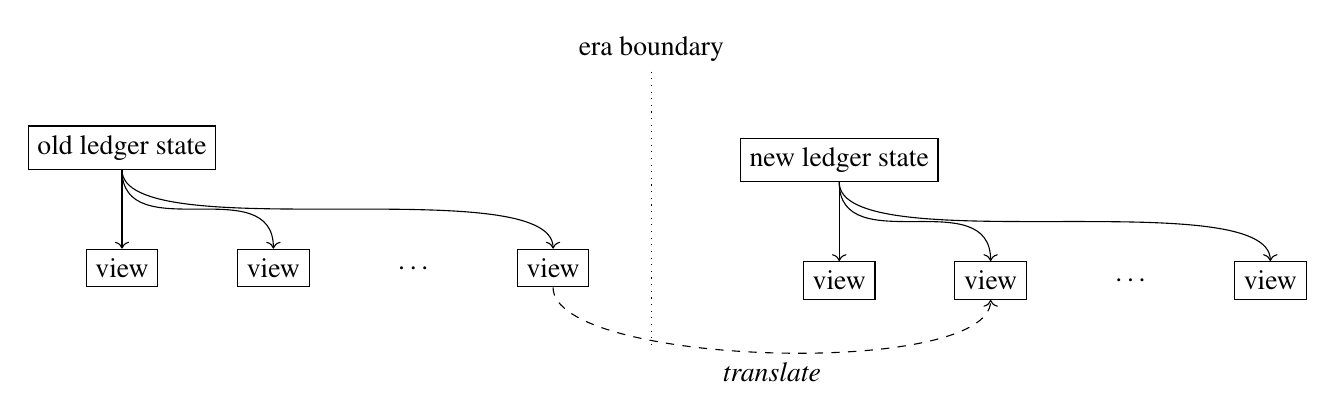
\begin{tikzpicture}[
square/.style={rectangle, draw},
]
% old ledger
\node[square] (Astate) {old ledger state};
\node[square] (Aview1) [below=of Astate] {view};
\node[square] (Aview2) [right=of Aview1] {view};
\node         (Adots)  [right=of Aview2] {$\ldots$};
\node[square] (AviewN) [right=of Adots]  {view};
\draw[->] (Astate.south) -- (Aview1.north);
\draw[->] (Astate.south) .. controls +(down:1cm) and +(up:1cm).. (Aview2.north);
\draw[->] (Astate.south) .. controls +(down:1cm) and +(up:1cm).. (AviewN.north);
%
% some intermediate nodes for positiiong
\node (AstateN) [above=of AviewN] {};
\node (mid) [right=of AstateN] {};
\node (midH) [above=of mid] {era boundary};
\node (midM) [below=of mid] {};
\node (midL) [below=of midM] {};
%
% new ledger
\node[square] (Bstate) [right=of mid] {new ledger state};
\node[square] (Bview1) [below=of Bstate] {view};
\node[square] (Bview2) [right=of Bview1] {view};
\node         (Bdots)  [right=of Bview2] {$\ldots$};
\node[square] (BviewN) [right=of Bdots]  {view};
\draw[->] (Bstate.south) -- (Bview1.north);
\draw[->] (Bstate.south) .. controls +(down:1cm) and +(up:1cm).. (Bview2.north);
\draw[->] (Bstate.south) .. controls +(down:1cm) and +(up:1cm).. (BviewN.north);
%
\draw[dotted] (midH) -- (midL);
\draw[->, dashed] (AviewN.south) .. controls +(down:1cm) and +(down:1cm) .. (Bview2.south) node[pos=0.5, below] {\emph{translate}};;
\end{tikzpicture}
\end{center}

The problem with this approach is that the ledger view only contains a small
subset of the ledger state; the old ledger state might contain information about
scheduled changes that should be taken into account when constructing the ledger
view in the new era, but the final ledger view in the old era might not have
that information.

Indeed, a moment's reflection reveals that this cannot be right the approach.
After all, we cannot step the ledger state; the dashed arrow in
%
\begin{center}
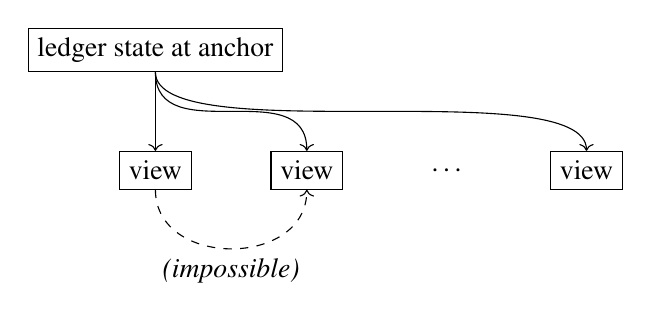
\begin{tikzpicture}[
square/.style={rectangle, draw},
]
\node[square] (state) {ledger state at anchor};
\node[square] (view1) [below=of state] {view};
\node[square] (view2) [right=of view1] {view};
\node         (dots)  [right=of view2] {$\ldots$};
\node[square] (viewN) [right=of dots]  {view};
\draw[->] (state.south) -- (view1.north);
\draw[->] (state.south) .. controls +(down:1cm) and +(up:1cm).. (view2.north);
\draw[->] (state.south) .. controls +(down:1cm) and +(up:1cm).. (viewN.north);
\draw[->, dashed] (view1.south) .. controls +(down:1cm) and +(down:1cm) .. (view2.south) node[pos=0.5, below] {\emph{(impossible)}};
\end{tikzpicture}
\end{center}
%
is not definable: scheduled changes are recorded in the ledger state, not in
the ledger view. If we cannot even do this \emph{within} an era, there is no
reason to assume it would be possible \emph{across} eras.

We cannot forecast directly from the old ledger state to the new era either:
this would result in a ledger view from the old era in the new era, violating
the invariant we discussed in \cref{hfc:ledger:invalid-states}.

Both approaches---forecasting the final old ledger state and then translating,
or forecasting directly across the era boundary and then translating---also
suffer from another problem: neither approach would compute correct forecast
bounds. Correct bounds depend on properties of both the old and the new ledger,
as well as the distance of the old ledger state to that final ledger view. For
example, if that final ledger view is right at the edge of the forecast range of
the old ledger state, we should not be able to give a forecast in the new era at
all.

Requiring a special forecasting function for each pair of eras of course in a
way is cheating: it pushes the complexity of doing this forecasting to the
specific ledgers that the HFC is instantiated at. As it turns out, however, this
function tends to be easy to define for any pair of concrete ledgers; it's just
hard to define in a completely general way.


\part{Testing}

\chapter{Reaching consensus}
\label{testing:consensus}

\section{Dire-but-not-to-dire}
\label{testing:dire}

We should mention the PBFT threshold here \cref{bft-paper}.

\chapter{The storage layer}
\label{testing:storage}


\part{Future Work}

\newcommand{\RequiredPeers}{\ensuremath{N_\mathit{rs}}}

% TODO: once verified, mark all these things are "not in the paper, but verified
% by the researchers"
\newcommand{\VerifiedByResearchers}{\todo{Verify}}

\chapter{Ouroboros Genesis}
\label{genesis}

\section{Introduction}





\pagebreak

\debugsep{OLD}

\section{Introduction}

\subsection{Chain length versus chain density}
\label{genesis:intro:length-vs-density}

The purpose of chain selection is to resolve temporary forks that arise from the
normal operation of the protocol (such as when there are multiple leaders in a
single slot), and---importantly---to distinguish honest chains from chains
forged by malicious nodes. It is not a priori clear why choosing longer chains
over shorter chains would help distinguish malicious chains from honest chains:
why would an honest chain be longer?

Recall that the leadership schedule is based on stake: a node's probability of
being elected a leader in a given slot is proportional to their stake. By
assumption, the malicious nodes in the system together have less stake than the
honest nodes; security of the system as a whole critically depends on the
presence of this honest majority. This means that when a malicious node extends
the chain they can only produce a chain with relatively few filled slots: the
honest chain will be \emph{denser}. At least, this will be true near the
intersection point: as we get further away from that intersection point, the
malicious node can attempt to influence the leadership schedule for future slots
to their advantage.

When all nodes in the system are up to date, they will all share the same chain,
except for blocks near the tips of those chains. Moreover, blocks with a slot
number ahead of the wall clock are considered invalid. This means that the only
way\footnote{The chain sync client does actually allow for some clock skew.
Headers that exceed the clock skew should not be taking into account in the
calculations that we discuss in this chapter.} for one chain to be longer than
another is by having more filled slots between the tip of the shared prefix and
``now'': in other words, they must be \emph{denser}.
%
\begin{center}
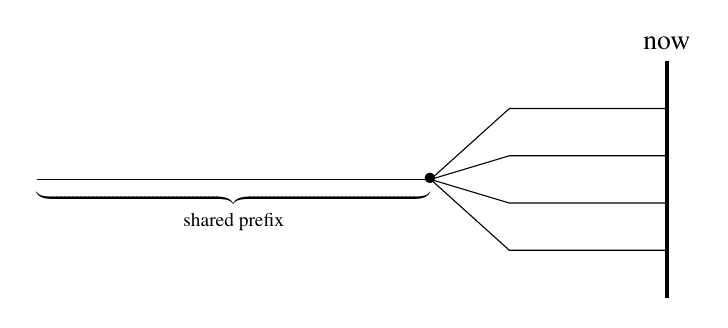
\begin{tikzpicture}
\draw (0,0) -- (5,0) coordinate(branch) node{$\bullet$} node[pos=0.5,below]{$\underbrace{\hspace{5cm}}_\text{shared prefix}$};
\draw (branch) -- ++(1,  0.9) -- ++(2,0);
\draw (branch) -- ++(1,  0.3) -- ++(2,0);
\draw (branch) -- ++(1, -0.3) -- ++(2,0);
\draw (branch) -- ++(1, -0.9) -- ++(2,0);
\draw [ultra thick] (8,-1.5) -- (8,1.5) node[above]{now};
\end{tikzpicture}
\end{center}
%
Conversely, the density of the fragment of a chain is only meaningful if that
fragment is long enough. Since the leadership election is a probabilistic
process, we only expect fragments to contain more slots signed by honest nodes
\emph{on average}, and we can only draw conclusions from density on long enough
fragments.

\subsection{Speculative mode}

Chain selection so far has been running in what we might call a ``speculative''
mode: when we see a new chain, we compare it to our current chain, and if we
prefer it, we adopt it (\cref{speculative-chain-selection}). This is speculative
in the sense that if we later see a second chain, we can change our mind about
adopting the first and adopt the second if that second chain is preferred over
the first.

The Praos chain selection rule (choose the longest chain) was explicitly
designed for a context in which all nodes in the network are present from the
very beginning (or somehow had one of the current chains when it joined) and are
always online. The Praos security analysis \cite{cryptoeprint:2017:573}
essentially shows that when the honest nodes in the system are all following
this protocol, they will end up with a common prefix, with disagreement possible
only about the most recent $k$ blocks. This means that nodes never need to roll
back past the tip of that common prefix; indeed, they \emph{should} not roll
back past that point, as this means they might adopt a chain forged by a
malicious node which is trying to trick them into believing some kind of
alternative history. This is the reason for the ``no rollback more than $k$
blocks'' rule in the Praos chain selection rule, as well as the justification
for the fact that much of the consensus layer is designed around the assumption
that there exists a maximum rollback distance.

In reality of course new nodes join the system all the time. This is problematic
for at least two reasons. First, within the consensus layer we don't see a
candidate chain's \emph{true} length; the length of a candidate we see depends
on how much of that candidate's chain we have downloaded\footnote{Nodes do
report their ``true length'', but since we have no way of verifying this
information until we have seen the entire chain, we can make no use of this
information for the purpose of chain selection.}. Defining chain
selection in terms of chain length, where our \emph{perceived} chain length
depends on what we decide to download, is obviously rather circular.

But the problem is more fundamental than that. Recall that chain
selection is running in speculative mode: we consider chains as we see them,
possibly changing our mind later by adopting a different chain. If a new node
sees a chain constructed by a malicious node and adopts it, \emph{it might be
stuck}: it is not difficult for an attacker to construct a chain that is longer
than $k$ blocks long (even if it will be sparser than the honest chain), and
once a node adopts such a chain, it will not be able to switch to the honest
chain anymore as this would involve a rollback of more than $k$ blocks.

\begin{figure}[p]
\hrule

\begin{tabular}{ll@{$\quad\Rightarrow\quad$}l}

(a)
&
&
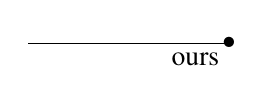
\begin{tikzpicture}[xscale=0.85]
\path (0, 0) coordinate (tip) node{$\bullet$} node[below left]{ours};
\draw (tip) + (-3,0) -- (tip);
\end{tikzpicture}
\\[1em]

(b)
&
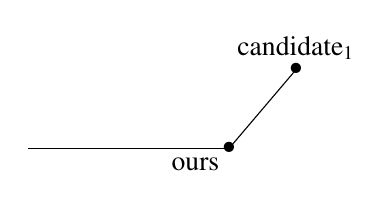
\begin{tikzpicture}[xscale=0.85]
\path (0, 0) coordinate (tip) node{$\bullet$} node[below left]{ours};
\draw (tip) + (-3,0) -- (tip);
\draw (tip) -- ++(1.0,  1.0) node{$\bullet$} coordinate (ab) node[above]{candidate$_1$};
\end{tikzpicture}
&
\begin{tikzpicture}[xscale=0.85]
\path (0, 0) coordinate (tip) node{$\bullet$};
\draw (tip) + (-3,0) -- (tip);
\draw (tip) -- ++(1.0,  1.0) node{$\bullet$} coordinate (ab) node[above]{ours};
\end{tikzpicture}
\\[1em]

(c)
&
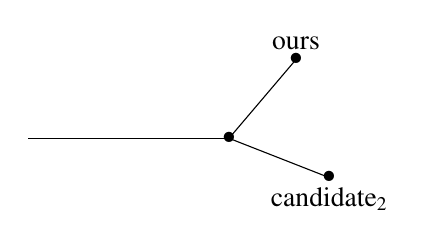
\begin{tikzpicture}[xscale=0.85]
\path (0, 0) coordinate (tip) node{$\bullet$};
\draw (tip) + (-3,0) -- (tip);
\draw (tip) -- ++(1.0,  1.0) node{$\bullet$} coordinate (ab) node[above]{ours};
\draw (tip) -- ++(1.5, -0.5) coordinate (cd) node{$\bullet$} node[below]{candidate$_2$};
\end{tikzpicture}
&
\begin{tikzpicture}[xscale=0.85]
\path (0, 0) coordinate (tip) node{$\bullet$};
\draw (tip) + (-3,0) -- (tip);
\draw (tip) -- ++(1.0,  1.0) node{$\bullet$} coordinate (ab);
\draw (tip) -- ++(1.5, -0.5) coordinate (cd) node{$\bullet$} node[below]{ours};
\end{tikzpicture}
\\[1em]

(d)
&
\begin{tikzpicture}[xscale=0.85]
\path (0, 0) coordinate (tip) node{$\bullet$};
\draw (tip) + (-3,0) -- (tip);
\draw (tip) -- ++(1.0,  1.0) node{$\bullet$} coordinate (ab);
\draw (tip) -- ++(1.5, -0.5) coordinate (cd) node{$\bullet$} node[below]{ours};
\draw (ab) -- ++(0.5,  0.5) -- ++(2.0, 0) node{$\bullet$} node[above]{candidate$_3$};
\end{tikzpicture}
&
\begin{tikzpicture}[xscale=0.85]
\path (0, 0) coordinate (tip) node{$\bullet$};
\draw (tip) + (-3,0) -- (tip);
\draw (tip) -- ++(1.0,  1.0) node{$\bullet$} coordinate (ab);
\draw (tip) -- ++(1.5, -0.5) coordinate (cd) node{$\bullet$};
\draw (ab) -- ++(0.5,  0.5) -- ++(2.0, 0) node{$\bullet$} node[above]{ours};
\end{tikzpicture}
\\[1em]

(e)
&
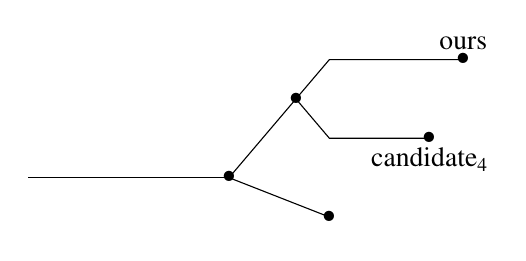
\begin{tikzpicture}[xscale=0.85]
\path (0, 0) coordinate (tip) node{$\bullet$};
\draw (tip) + (-3,0) -- (tip);
\draw (tip) -- ++(1.0,  1.0) node{$\bullet$} coordinate (ab);
\draw (tip) -- ++(1.5, -0.5) coordinate (cd) node{$\bullet$};
\draw (ab) -- ++(0.5,  0.5) -- ++(2.0, 0) node{$\bullet$} node[above]{ours};
\draw (ab) -- ++(0.5, -0.5) -- ++(1.5, 0) node{$\bullet$} node[below]{candidate$_4$};
\end{tikzpicture}
&
\begin{tikzpicture}[xscale=0.85]
\path (0, 0) coordinate (tip) node{$\bullet$};
\draw (tip) + (-3,0) -- (tip);
\draw (tip) -- ++(1.0,  1.0) node{$\bullet$} coordinate (ab);
\draw (tip) -- ++(1.5, -0.5) coordinate (cd) node{$\bullet$};
\draw (ab) -- ++(0.5,  0.5) -- ++(2.0, 0) node{$\bullet$} node[above]{ours};
\draw (ab) -- ++(0.5, -0.5) -- ++(1.5, 0) node{$\bullet$};
\end{tikzpicture}
\\[1em]

(f)
&
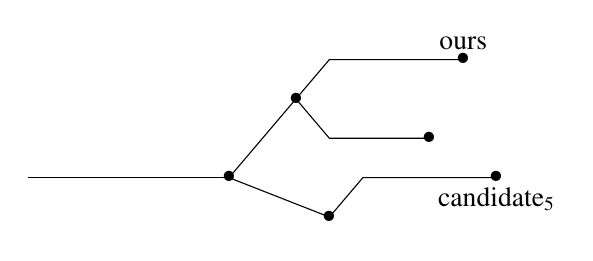
\begin{tikzpicture}[xscale=0.85]
\path (0, 0) coordinate (tip) node{$\bullet$};
\draw (tip) + (-3,0) -- (tip);
\draw (tip) -- ++(1.0,  1.0) node{$\bullet$} coordinate (ab);
\draw (tip) -- ++(1.5, -0.5) coordinate (cd) node{$\bullet$};
\draw (ab) -- ++(0.5,  0.5) -- ++(2.0, 0) node{$\bullet$} node[above]{ours};
\draw (ab) -- ++(0.5, -0.5) -- ++(1.5, 0) node{$\bullet$};
\draw (cd) -- ++(0.5,  0.5) -- ++(2.0, 0) node{$\bullet$} node[below]{candidate$_5$};
\end{tikzpicture}
&
\begin{tikzpicture}[xscale=0.85]
\path (0, 0) coordinate (tip) node{$\bullet$};
\draw (tip) + (-3,0) -- (tip);
\draw (tip) -- ++(1.0,  1.0) node{$\bullet$} coordinate (ab);
\draw (tip) -- ++(1.5, -0.5) coordinate (cd) node{$\bullet$};
\draw (ab) -- ++(0.5,  0.5) -- ++(2.0, 0) node{$\bullet$};
\draw (ab) -- ++(0.5, -0.5) -- ++(1.5, 0) node{$\bullet$};
\draw (cd) -- ++(0.5,  0.5) -- ++(2.0, 0) node{$\bullet$} node[below]{ours};
\end{tikzpicture}
\\
\end{tabular}

\hrule
\caption{\label{speculative-chain-selection}Speculative chain selection}
\end{figure}

\subsection{Genesis rule}

Any node with non-zero stake can easily construct chains of arbitrary length,
but such chains will necessarily be sparse. Indeed, as we argued above,
chains constructed by malicious nodes cannot be denser (on a sufficiently
long fragment) than the honest chain.

The \emph{Genesis chain selection rule}, designed to cope with new nodes joining
the network, therefore compares chains on density whenever possible, defaulting
to comparing chain length only if there aren't enough blocks to do a meaningful
density comparison. The size of this ``density window'' is a parameter to the
rule known as $s$; as it turns out, however, we must pick $s$ such that the
probability of a $k$-common prefix violation within an $s$ sized window is
neglible:\VerifiedByResearchers{}

\begin{definition}[Genesis window size]
\label{default-genesis-window}
The genesis window size $s$ must be equal to the stability window;
that is $s = 3k / f$.
\end{definition}

The genesis rule we will use in this chapter differs slightly from the one from
the original paper:

\begin{definition}[Genesis rule]
\label{genesis:rule}
A candidate chain is preferred over our current chain if

\begin{itemize}
\item The intersection between the candidate chain and our chain is \textbf{at
least $s$ slots} back from the tip of our chain, and the candidate chain is
\textbf{denser} in a window of $s$ slots at the intersection, or

\item The intersection between the candidate chain and our chain is \textbf{less
than $s$ slots} back from the tip of our chain, and the candidate chain is
strictly \textbf{longer} than our chain.
\end{itemize}

\end{definition}

\subsection{Conservative mode}
\label{genesis:intro:conservative}

The rule as defined in \cref{genesis:rule} is problematic for consensus:
\emph{it no longer imposes a maximum rollback}. We depend on this maximum
rollback in many ways
(\cref{consensus:overview:k,storage:components,chainsyncclient:validation,chainsyncclient:forecasting}
and others), and we will want to \emph{continue} to depend on it. Less
fundamentally, but nonetheless importantly, it also doesn't fit very well with
our look-at-the-tip-only approach (\cref{consensus:overview:chainsel}). We will
therefore treat the genesis chain selection rule as a special case.

Specifically, we will switch from the default speculative chain selection mode
to a \emph{conservative} chain selection mode. We will see the details of how
this mode works later in this chapter, but the intuition is that rather than
considering and possibly adopting chains as we encounter them, we instead wait,
collecting enough information to fill a ``look-ahead window'' which will allow
us to make progress, either discarding candidates or adopting blocks.
Critically, the decisions we make in conservative mode are not subject to
rollback: we wait until we can be sure. \Cref{conservative-chain-selection}
illustrates what this might look like.

The security analysis of the genesis chain selection rule includes a theorem
\cite[Theorem 2]{cryptoeprint:2018:378} that says that it is still true that
\emph{when nodes are up to date} they will never need to roll back more than $k$
blocks. We can use this theorem to justify switching from the conservative
mode back to the speculative mode. Since blocks ahead of the wall clock are
considered invalid, we can use the current slot number (according to the
wallclock) to estimate if we are within $k$ blocks from the longest chain
in the network. We cannot do better than an estimate because we might not know
the density of that chain. The latest point we can switch is $s$ slots away
from the wall clock: any later and we would not be able to look-ahead far enough
to apply the genesis rule (see \cref{genesis:rules}, especially
\cref{{genesis:insufficient-blocks}}). As it turns out, we will need to switch a
little sooner than that; we will discuss the details in
\cref{genesis:insufficient-blocks,genesis:switch-over-point}.

The switch over point does not change the chain selection rule itself: even when
we are in speculative mode, we will still apply the genesis rule as defined in
\cref{genesis:rule}, comparing density or length depending on the intersection
point; we will merely use Theorem 2 of the genesis security analysis to justify
imposing the standard maximum rollback of $k$ blocks.

\begin{figure}[p]
\hrule

\begin{tabular}{ll@{$\quad\Rightarrow\quad$}l}
a &&
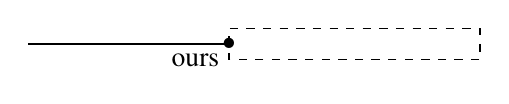
\begin{tikzpicture}[xscale=0.85]
\path (0, 0) coordinate (tip) node{$\bullet$} node[below left]{ours};
\draw [dashed] (tip) -- ++(0, 0.2) -- ++(3.75, 0) -- ++(0, -0.4) -- ++(-3.75, 0) -- cycle;
\draw (tip) + (-3,0) -- (tip);
\end{tikzpicture}
\\

b &&
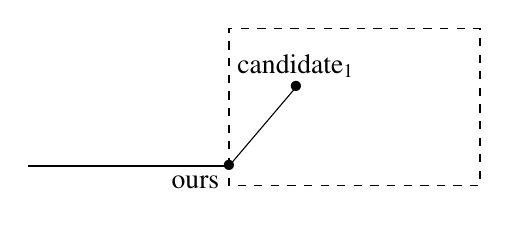
\begin{tikzpicture}[xscale=0.85]
\path (0, 0) coordinate (tip) node{$\bullet$} node[below left]{ours};
\draw [dashed] (tip) -- ++(0, 1.75) -- ++(3.75, 0) -- ++(0, -2) -- ++(-3.75, 0) -- cycle;
\draw (tip) + (-3,0) -- (tip);
\draw (tip) -- ++(1.0,  1.0) node{$\bullet$} coordinate (ab) node[above]{candidate$_1$};
\end{tikzpicture}
\\

c &&
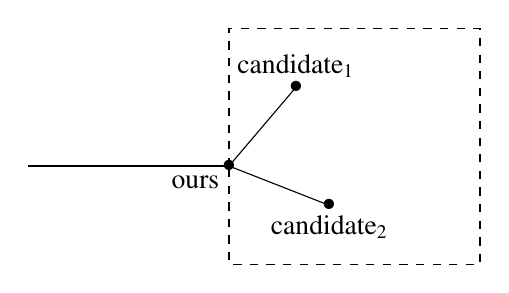
\begin{tikzpicture}[xscale=0.85]
\path (0, 0) coordinate (tip) node{$\bullet$} node[below left]{ours};
\draw [dashed] (tip) -- ++(0, 1.75) -- ++(3.75, 0) -- ++(0, -3) -- ++(-3.75, 0) -- cycle;
\draw (tip) + (-3,0) -- (tip);
\draw (tip) -- ++(1.0,  1.0) node{$\bullet$} coordinate (ab) node[above]{candidate$_1$};
\draw (tip) -- ++(1.5, -0.5) coordinate (cd) node{$\bullet$} node[below]{candidate$_2$};
\end{tikzpicture}
\\

d &&
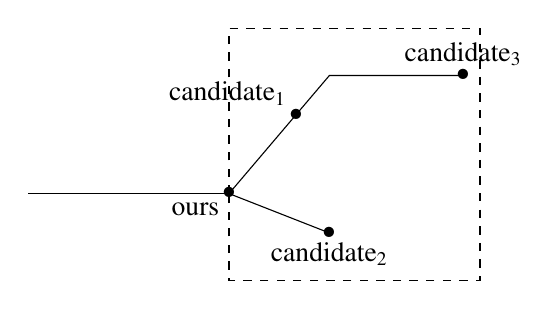
\begin{tikzpicture}[xscale=0.85]
\path (0, 0) coordinate (tip) node{$\bullet$} node[below left]{ours};
\draw [dashed] (tip) -- ++(0, 2.1) -- ++(3.75, 0) -- ++(0, -3.2) -- ++(-3.75, 0) -- cycle;
\draw (tip) + (-3,0) -- (tip);
\draw (tip) -- ++(1.0,  1.0) node{$\bullet$} coordinate (ab) node[above left]{candidate$_1$};
\draw (tip) -- ++(1.5, -0.5) coordinate (cd) node{$\bullet$} node[below]{candidate$_2$};
\draw (ab) -- ++(0.5,  0.5) -- ++(2.0, 0) node{$\bullet$} node[above]{candidate$_3$};
\end{tikzpicture}
\\

e &&
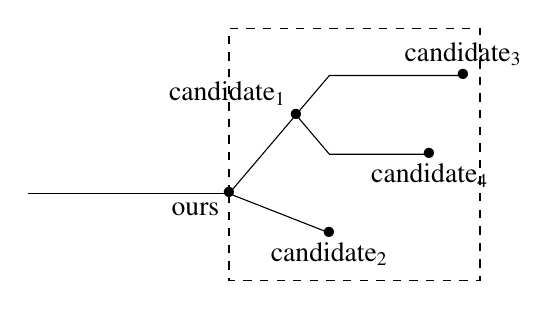
\begin{tikzpicture}[xscale=0.85]
\path (0, 0) coordinate (tip) node{$\bullet$} node[below left]{ours};
\draw [dashed] (tip) -- ++(0, 2.1) -- ++(3.75, 0) -- ++(0, -3.2) -- ++(-3.75, 0) -- cycle;
\draw (tip) + (-3,0) -- (tip);
\draw (tip) -- ++(1.0,  1.0) node{$\bullet$} coordinate (ab) node[above left]{candidate$_1$};
\draw (tip) -- ++(1.5, -0.5) coordinate (cd) node{$\bullet$} node[below]{candidate$_2$};
\draw (ab) -- ++(0.5,  0.5) -- ++(2.0, 0) node{$\bullet$} node[above]{candidate$_3$};
\draw (ab) -- ++(0.5, -0.5) -- ++(1.5, 0) node{$\bullet$} node[below]{candidate$_4$};
\end{tikzpicture}
\\

f &&
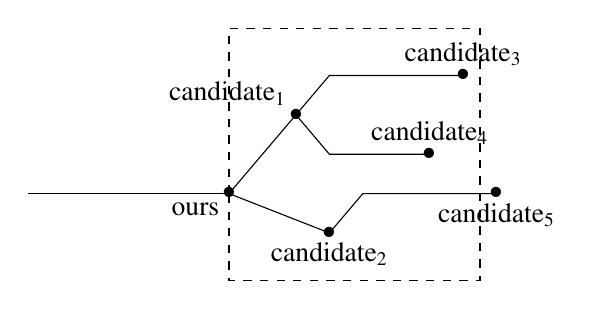
\begin{tikzpicture}[xscale=0.85]
\path (0, 0) coordinate (tip) node{$\bullet$}  node[below left]{ours};
\draw [dashed] (tip) -- ++(0, 2.1) -- ++(3.75, 0) -- ++(0, -3.2) -- ++(-3.75, 0) -- cycle;
\draw (tip) + (-3,0) -- (tip);
\draw (tip) -- ++(1.0,  1.0) node{$\bullet$} coordinate (ab) node[above left]{candidate$_1$};
\draw (tip) -- ++(1.5, -0.5) coordinate (cd) node{$\bullet$} node[below]{candidate$_2$};
\draw (ab) -- ++(0.5,  0.5) -- ++(2.0, 0) node{$\bullet$} node[above]{candidate$_3$};
\draw (ab) -- ++(0.5, -0.5) -- ++(1.5, 0) node{$\bullet$}  node[above]{candidate$_4$};
\draw (cd) -- ++(0.5,  0.5) -- ++(2.0, 0) node{$\bullet$} node[below]{candidate$_5$};
\end{tikzpicture}
\\

g &&
\begin{tikzpicture}[xscale=0.85]
\path (0, 0) coordinate (tip) node{$\bullet$};
\draw [dashed] (tip) -- ++(0, 2.1) -- ++(3.75, 0) -- ++(0, -3.2) -- ++(-3.75, 0) -- cycle;
\draw (tip) + (-3,0) -- (tip);
\draw [dotted] (tip) -- ++(1.0,  1.0) coordinate (ab);
\draw (tip) -- ++(1.5, -0.5) coordinate (cd) node{$\bullet$} node[below]{ours};
\draw [dotted] (ab) -- ++(0.5,  0.5) -- ++(2.0, 0);
\draw [dotted] (ab) -- ++(0.5, -0.5) -- ++(1.5, 0);
\draw (cd) -- ++(0.5,  0.5) -- ++(2.0, 0) node{$\bullet$} node[below]{candidate$_5$};
\end{tikzpicture}
\\

\end{tabular}

\hrule
\caption{\label{conservative-chain-selection}Conservative chain selection}
\end{figure}

\section{Applying the genesis rule in conservative mode}
\label{genesis:rules}

In this section we will show the rules that we will use to implement the
genesis chain selection rule whilst in conservative mode. Throughout we will
rely critically on the following assumption:

\begin{assumption}[Representative sample]
There exists some threshold $\RequiredPeers$ such that if we see the chains of
at least $\RequiredPeers$ peers, we have seen a representative sample of
\emph{all} relevant chains available in the network at that time; there are no
other chains in the network that we do not know about but \emph{should} know
about.
\end{assumption}

This implies that an attacker cannot \emph{eclipse} us; this is something
outside the scope of the consensus layer, and must be guaranteed by the network
layer (probably by a probabilistic way of choosing peers).

We will set the size of our ``look-ahead window'' to be precisely $s$; that is,
we will set the size of the look-ahead window used for conservative chain
selection to be exactly equal to the genesis window (we will see shortly why
this is a suitable choice). There are now two possibilities: either all chains
in our window share a common prefix, or they don't and they fork at the start of
the window. We will consider these two cases separately.

\pagebreak

\subsection{Fork: discard}
\label{genesis:discard}

Suppose that $\RequiredPeers = 4$, and our window looks like this:
%
\begin{center}
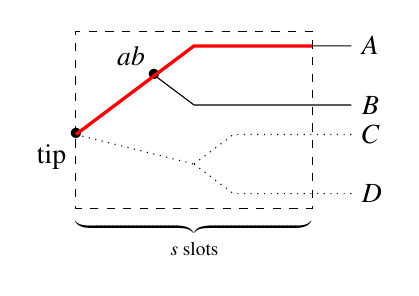
\begin{tikzpicture}[yscale=0.75]
\path (0, 0) coordinate (tip) node{$\bullet$} node[below left]{tip};
\draw (tip) -- ++(1.0,  1.0) coordinate (ab) node{$\bullet$} node[above left]{$ab$};
\draw [dotted] (tip) -- ++(1.5, -0.5) coordinate (cd);
\draw (ab) -- ++(0.5,  0.5) -- ++(2.0, 0) coordinate(A) node[right]{$A$};
\draw (ab) -- ++(0.5, -0.5) -- ++(2.0, 0) node[right]{$B$};
\draw [dotted] (cd) -- ++(0.5,  0.5) -- ++(1.5, 0) node[right]{$C$};
\draw [dotted] (cd) -- ++(0.5, -0.5) -- ++(1.5, 0) node[right]{$D$};
\draw [dashed]
     (tip)
  -- ++(0, 1.75)
  -- ++(3, 0)
  -- ++(0, -3)
  -- ++(-3, 0) node[pos=0.5, below]{$\underbrace{\hspace{3cm}}_{\text{$s$ slots}}$}
  -- cycle;

%%%%%%%%%%%%%%%%%%%%%%%%%%%%%%%%%%%%%%%%

\draw [red, very thick] (tip) -- (ab) -- ++(0.5,  0.5) -- ++(1.5, 0);
\end{tikzpicture}
\end{center}
%
where $A \ldots D$ are (filled) slots on different forks, at least  $s$ slots
away from the intersection point. The thick red line is marking the densest
chain section within the window. Consider what the normal genesis rule would do:
%
\begin{itemize}
\item
Suppose we saw candidate $A$ first, and later discovered $C$ or $D$: since the
intersection with these chains is at least $s$ slots back from the tip of
$A$, we would compare the density within a window of $s$ slots from the
intersection point, and then pick the  denser chain. Since that denser chain is
$A$, we would stick with $A$.
\item
Conversely, if our current chain was $C$ or $D$, and we would discover $A$, we
would once again compare the density at the intersection point (because  the
distance from the tip of $C$ or $D$ to the intersection point is also at least
$s$ slots), find that $A$ is denser, and so switch to $A$.
\end{itemize}
%
Either way, we would end up choosing $A$. The window of $s$ slots that is relevant
to distinguish between $A$ and $C$ or $D$ is \emph{precisely} the window we are
currently looking at; this means that we can \emph{discard} candidates $C$
and $D$ at this point; we will never be interested in them.

We cannot choose between $A$ and $B$ yet, because for that we would need to see
the window anchored at the \emph{later} intersection point between those two
chains. It is important that we compare density only \emph{at the intersection
point}. In case that isn't obvious, in the rest of this section we will consider
an example that will hopefully clarify it. Suppose the chain is growing
normally, then a malicious node with some stake intentionally skips their slot,
after which the chain continues to grow again:
%
\begin{center}
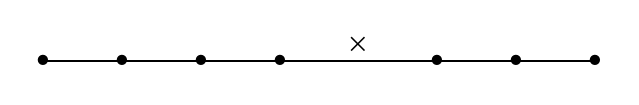
\begin{tikzpicture}[yscale=0.75]
\draw
       (0,0) node{$\bullet$}
  -- ++(1,0) node{$\bullet$}
  -- ++(1,0) node{$\bullet$}
  -- ++(1,0) node{$\bullet$}
  -- ++(1,0) node[above]{$\times$}
  -- ++(1,0) node{$\bullet$}
  -- ++(1,0) node{$\bullet$}
  -- ++(1,0) node{$\bullet$};
\end{tikzpicture}
\end{center}
%
It is now trivial for the attacker to create an alternative chain that
\emph{does} have a block in that slot; if other nodes switch to the denser chain
the moment they see a window of $s$ slots that is denser, they would adopt the
attacker's chain; after all, it has one more block in the window than the real
chain does:
%
\begin{center}
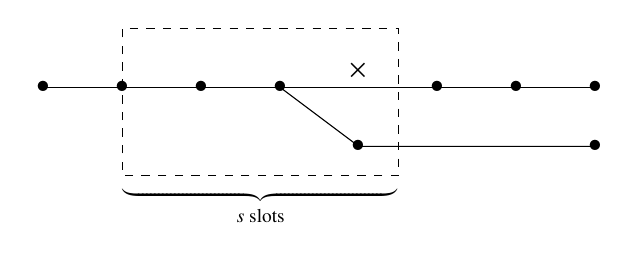
\begin{tikzpicture}[yscale=0.75]
\draw
       (0,0) node{$\bullet$}
  -- ++(1,0) node{$\bullet$} coordinate(s-anchor)
  -- ++(1,0) node{$\bullet$}
  -- ++(1,0) node{$\bullet$} coordinate(branch)
  -- ++(1,0) node[above]{$\times$}
  -- ++(1,0) node{$\bullet$}
  -- ++(1,0) node{$\bullet$}
  -- ++(1,0) node{$\bullet$};
\draw
       (branch)
  -- ++(1, -1) node{$\bullet$}
  -- ++(3,  0) node{$\bullet$};
\draw [dashed]
     (s-anchor)
  -- ++(0,1)
  -- ++(3.5,0)
  -- ++(0,-2.5)
  -- ++(-3.5,0) node[below, pos=0.5]{$\underbrace{\hspace{3.5cm}}_{\text{$s$ slots}}$}
  -- cycle;
\end{tikzpicture}
\end{center}
%
Instead, we must wait until we make such a comparison until we have reached
the intersection point:
%
\begin{center}
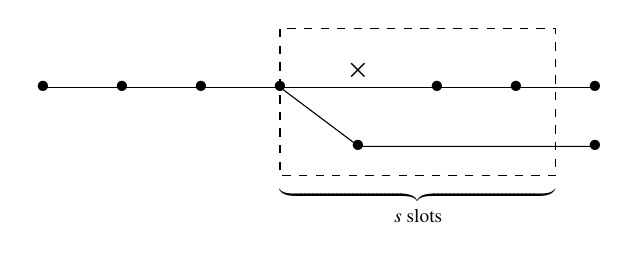
\begin{tikzpicture}[yscale=0.75]
\draw
       (0,0) node{$\bullet$}
  -- ++(1,0) node{$\bullet$}
  -- ++(1,0) node{$\bullet$}
  -- ++(1,0) node{$\bullet$} coordinate(branch)
  -- ++(1,0) node[above]{$\times$}
  -- ++(1,0) node{$\bullet$}
  -- ++(1,0) node{$\bullet$}
  -- ++(1,0) node{$\bullet$};
\draw
       (branch)
  -- ++(1, -1) node{$\bullet$}
  -- ++(3,  0) node{$\bullet$};
\draw [dashed]
     (branch)
  -- ++(0,1)
  -- ++(3.5,0)
  -- ++(0,-2.5)
  -- ++(-3.5,0) node[below, pos=0.5]{$\underbrace{\hspace{3.5cm}}_{\text{$s$ slots}}$}
  -- cycle;
\end{tikzpicture}
\end{center}
%
Since the attacker does not have sufficient stake, if we \emph{now} compare the
attacker's chain to the real chain, we will find that the attacker's chain is
less dense and nodes will therefore not select it. If the attacker creates
another fork earlier on the chain, then we will resolve that fork
when we encounter it using a window of $s$ slots \emph{anchored at that fork},
and then later resolve the second fork using a \emph{different} window of
$s$ slots, anchored at the second fork:
%
\begin{center}
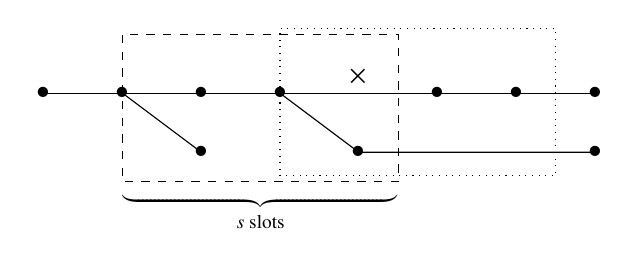
\begin{tikzpicture}[yscale=0.75]
\draw
       (0,0) node{$\bullet$}
  -- ++(1,0) node{$\bullet$} coordinate(s-anchor)
  -- ++(1,0) node{$\bullet$}
  -- ++(1,0) node{$\bullet$} coordinate(branch)
  -- ++(1,0) node[above]{$\times$}
  -- ++(1,0) node{$\bullet$}
  -- ++(1,0) node{$\bullet$}
  -- ++(1,0) node{$\bullet$};
\draw
       (branch)
  -- ++(1, -1) node{$\bullet$}
  -- ++(3,  0) node{$\bullet$};
\draw
       (s-anchor)
  -- ++(1, -1) node{$\bullet$};
\draw [dashed]
     (s-anchor)
  -- ++(0,1)
  -- ++(3.5,0)
  -- ++(0,-2.5)
  -- ++(-3.5,0) node[below, pos=0.5]{$\underbrace{\hspace{3.5cm}}_{\text{$s$ slots}}$}
  -- cycle;
\draw [dotted]
     (branch) ++ (0, 0.1)
  -- ++(0,1)
  -- ++(3.5,0)
  -- ++(0,-2.5)
  -- ++(-3.5,0)
  -- cycle;
\end{tikzpicture}
\end{center}

\subsection{Common prefix: adopt}
\label{genesis:adopt}

If there is no fork point at the start of the window, then by definition
all candidates must share some common prefix:
%
\begin{center}
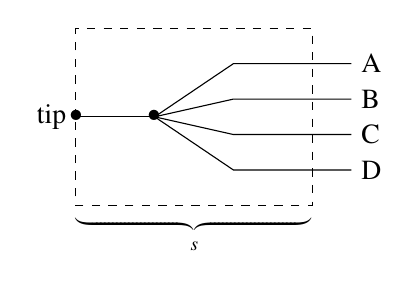
\begin{tikzpicture}[yscale=0.75]
\path (0, 0) coordinate (tip) node{$\bullet$};
\draw (tip) -- ++(1.0,  0.0) coordinate (branch) node{$\bullet$};
\draw (branch) -- ++(1.0,  0.9) -- ++ (1.5, 0) node[right]{A};
\draw (branch) -- ++(1.0,  0.3) -- ++ (1.5, 0) node[right]{B};
\draw (branch) -- ++(1.0, -0.3) -- ++ (1.5, 0) node[right]{C};
\draw (branch) -- ++(1.0, -0.9) -- ++ (1.5, 0) node[right]{D};

%%%%%%%%%%%%%%%%%%%%%%%%%%%%%%%%%%%%%%%%

\node [left] at (tip) {tip};
\draw [dashed]
     (tip)
  -- ++(0, 1.5)
  -- ++(3, 0)
  -- ++(0, -3)
  -- ++(-3, 0) node[pos=0.5, below]{$\underbrace{\hspace{3cm}}_s$}
  -- cycle;

\end{tikzpicture}
\end{center}
%
Since by assumption the candidates in our window are a representative sample
of all chains in the network, this means that \emph{all} chains share this
common prefix, and so we can for \emph{sure} adopt those blocks into our
own chain, moving up our window:
%
\begin{center}
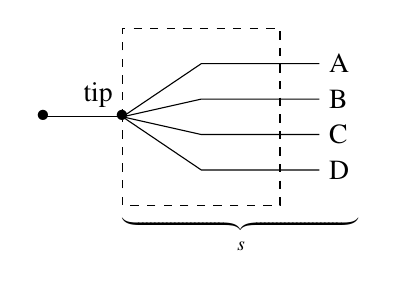
\begin{tikzpicture}[yscale=0.75]
\path (0, 0) coordinate (tip) node{$\bullet$};
\draw (tip) -- ++(1.0,  0.0) coordinate (branch) node{$\bullet$};
\draw (branch) -- ++(1.0,  0.9) -- ++ (1.5, 0) node[right]{A};
\draw (branch) -- ++(1.0,  0.3) -- ++ (1.5, 0) node[right]{B};
\draw (branch) -- ++(1.0, -0.3) -- ++ (1.5, 0) node[right]{C};
\draw (branch) -- ++(1.0, -0.9) -- ++ (1.5, 0) node[right]{D};

%%%%%%%%%%%%%%%%%%%%%%%%%%%%%%%%%%%%%%%%

\node [above left] at (branch) {tip};
\draw [dashed]
     (branch)
  -- ++(0, 1.5)
  -- ++(2, 0)
  -- ++(0, -3)
  -- ++(-2, 0)  node[pos=0.25, below]{$\underbrace{\hspace{3cm}}_s$}
  -- cycle;
\end{tikzpicture}
\end{center}

When we move up the window, we have to wait for it to fill again; we will
discuss this in detail in \cref{genesis:insufficient-blocks}.

\subsection{General case}

Notice that we only adopt blocks when they appear on \emph{all} relevant
chains in the system (\cref{genesis:adopt}). This means that we will never have
to roll such blocks back: everything we adopt we are certain about and will
never change our mind about.

This allows us to generalise the pictures from the previous two sections
slightly. Rather than having the window anchored at genesis, it is
anchored at the tip of a chain of blocks that we are sure about; so for the
fork/discard case (\cref{genesis:discard}), the generalisation looks like
%
\begin{center}
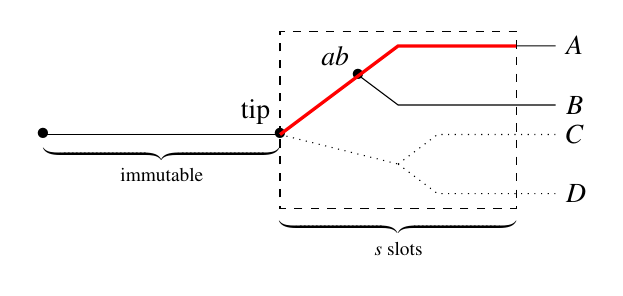
\begin{tikzpicture}[yscale=0.75]
\path (0, 0) coordinate (tip) node{$\bullet$} node[above left]{tip};
\draw (tip) -- ++(1.0,  1.0) coordinate (ab) node{$\bullet$} node[above left]{$ab$};
\draw [dotted] (tip) -- ++(1.5, -0.5) coordinate (cd);
\draw (ab) -- ++(0.5,  0.5) -- ++(2.0, 0) coordinate(A) node[right]{$A$};
\draw (ab) -- ++(0.5, -0.5) -- ++(2.0, 0) node[right]{$B$};
\draw [dotted] (cd) -- ++(0.5,  0.5) -- ++(1.5, 0) node[right]{$C$};
\draw [dotted] (cd) -- ++(0.5, -0.5) -- ++(1.5, 0) node[right]{$D$};
\draw [dashed]
     (tip)
  -- ++(0, 1.75)
  -- ++(3, 0)
  -- ++(0, -3)
  -- ++(-3, 0) node[pos=0.5, below]{$\underbrace{\hspace{3cm}}_{\text{$s$ slots}}$}
  -- cycle;

%%%%%%%%%%%%%%%%%%%%%%%%%%%%%%%%%%%%%%%%

\draw [red, very thick] (tip) -- (ab) -- ++(0.5,  0.5) -- ++(1.5, 0);
\draw (tip) + (-3,0) node{$\bullet$} -- (tip) node[pos=0.5, below]{$\underbrace{\hspace{3cm}}_\text{immutable}$};
\end{tikzpicture}
\end{center}
%
Similarly, for the common prefix/adopt case (\cref{genesis:adopt}), it looks like
%
\begin{center}
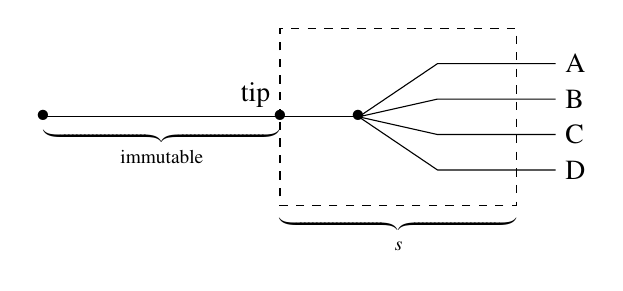
\begin{tikzpicture}[yscale=0.75]
\path (0, 0) coordinate (tip) node{$\bullet$};
\draw (tip) -- ++(1.0,  0.0) coordinate (branch) node{$\bullet$};
\draw (branch) -- ++(1.0,  0.9) -- ++ (1.5, 0) node[right]{A};
\draw (branch) -- ++(1.0,  0.3) -- ++ (1.5, 0) node[right]{B};
\draw (branch) -- ++(1.0, -0.3) -- ++ (1.5, 0) node[right]{C};
\draw (branch) -- ++(1.0, -0.9) -- ++ (1.5, 0) node[right]{D};

%%%%%%%%%%%%%%%%%%%%%%%%%%%%%%%%%%%%%%%%

\node [above left] at (tip) {tip};
\draw [dashed]
     (tip)
  -- ++(0, 1.5)
  -- ++(3, 0)
  -- ++(0, -3)
  -- ++(-3, 0) node[pos=0.5, below]{$\underbrace{\hspace{3cm}}_s$}
  -- cycle;
\draw (tip) + (-3,0) node{$\bullet$} -- (tip) node[pos=0.5, below]{$\underbrace{\hspace{3cm}}_\text{immutable}$};

\end{tikzpicture}
\end{center}

\subsection{Insufficient peers}

When we have not yet connected to at least $\RequiredPeers$ peers, neither of
our two rules can be applied. Consider again the rule that deals with forks:
%
\begin{center}
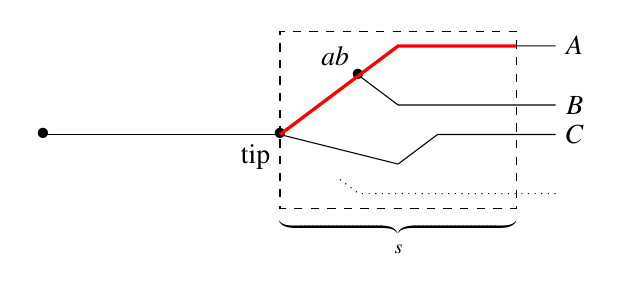
\begin{tikzpicture}[yscale=0.75]
\path (0, 0) coordinate (tip) node{$\bullet$} node[below left]{tip};
\draw (tip) -- ++(1.0,  1.0) coordinate (ab) node{$\bullet$} node[above left]{$ab$};
\draw (tip) -- ++(1.5, -0.5) coordinate (cd);
\draw (ab) -- ++(0.5,  0.5) -- ++(2.0, 0) node[right]{$A$};
\draw (ab) -- ++(0.5, -0.5) -- ++(2.0, 0) node[right]{$B$};
\draw (cd) -- ++(0.5,  0.5) -- ++(1.5, 0) node[right]{$C$};
\path (cd) -- ++(0.5, -0.5) -- ++(1.5, 0) coordinate (D);

\draw [dashed]
     (tip)
  -- ++(0, 1.75)
  -- ++(3, 0)
  -- ++(0, -3)
  -- ++(-3, 0) node[pos=0.5, below]{$\underbrace{\hspace{3cm}}_s$}
  -- cycle;
\draw [dotted] (D) -- ++(-2.5,0) -- ++(-0.25,0.25);

\draw [red, very thick] (tip) -- (ab) -- ++(0.5,  0.5) -- ++(1.5, 0) ;
\draw (tip) + (-3,0) node{$\bullet$} -- (tip);
\end{tikzpicture}
\end{center}
%
Since we don't know the density of the missing chain $D$, it's not sound to
conclude that $A$ is the densest. Similarly, in the rule for a common prefix,
%
\begin{center}
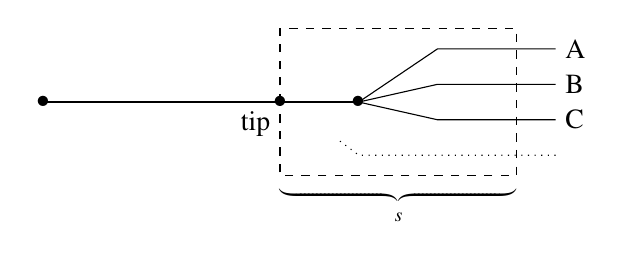
\begin{tikzpicture}[yscale=0.75]
\path (0, 0) coordinate (tip) node{$\bullet$};
\draw (tip) -- ++(1.0,  0.0) coordinate (branch) node{$\bullet$};
\draw (branch) -- ++(1.0,  0.9) -- ++ (1.5, 0) node[right]{A};
\draw (branch) -- ++(1.0,  0.3) -- ++ (1.5, 0) node[right]{B};
\draw (branch) -- ++(1.0, -0.3) -- ++ (1.5, 0) node[right]{C};
\path (branch) -- ++(1.0, -0.9) -- ++ (1.5, 0) coordinate(D);

\draw [dotted] (D) -- ++(-2.5,0) -- ++(-0.25,0.25);
\node [below left] at (tip) {tip};
\draw [dashed]
     (tip)
  -- ++(0, 1.25)
  -- ++(3, 0)
  -- ++(0, -2.5)
  -- ++(-3, 0) node[pos=0.5, below]{$\underbrace{\hspace{3cm}}_s$}
  -- cycle;
\draw (tip) + (-3,0) node{$\bullet$} -- (tip);

\end{tikzpicture}
\end{center}
%
we don't know if the missing chain $D$ \emph{also} starts with the same block,
and so we don't know if the common prefix rule can be applied.

\subsection{Insufficient blocks}
\label{genesis:insufficient-blocks}

We can make more progress in the situation where we \emph{do} have all the peers
we need, but their chains might not fill the look-ahead window. The rule for
common prefix is the simpler case:
%
\begin{center}
\begin{tikzpicture}[yscale=0.75]
\path (0, 0) coordinate (tip) node{$\bullet$};
\draw (tip) -- ++(1.0,  0.0) coordinate (branch) node{$\bullet$};
\draw (branch) -- ++(1.0,  0.9) -- ++ (1.5, 0) node[right]{A};
\draw (branch) -- ++(1.0,  0.3) -- ++ (1.5, 0) node[right]{B};
\draw (branch) -- ++(1.0, -0.3) -- ++ (1.5, 0) node[right]{C};
\draw (branch) -- ++(1.0, -0.9) coordinate(D) node{$\bullet$} node[below]{D};
\draw [dashed] (D) -- ++ (1.5, 0);

\node [below left] at (tip) {tip};
\draw [dashed]
     (tip)
  -- ++(0, 1.25)
  -- ++(3, 0)
  -- ++(0, -3)
  -- ++(-3, 0) node[pos=0.5, below]{$\underbrace{\hspace{3cm}}_s$}
  -- cycle;
\draw (tip) + (-3,0) node{$\bullet$} -- (tip);

\end{tikzpicture}
\end{center}
%
Even though we have not yet seen enough of chain $D$ to fill the window, it does
not matter; by assumption, if we see at least $\RequiredPeers$ chains, we have
seen all relevant chains in the network, and if all of those chains start with
the same block, we can definitely adopt that block. From a practical
perspective, this is an important special case: under normal circumstances, we
expect all peers in the network to report the exact same chain, at least for all
but the last few of the millions of blocks on their chains. This means that we
can adopt blocks almost as soon as we see them during syncing.

\pagebreak

The situation is more subtle in the case of a fork:
%
\begin{center}
\begin{tikzpicture}[yscale=0.75]
\path (0, 0) coordinate (tip) node{$\bullet$} node[below left]{tip};
\draw (tip) -- ++(1.0,  1.0) coordinate (ab) node{$\bullet$} node[above left]{$ab$};
\draw (tip) -- ++(1.5, -0.5) coordinate (cd);
\draw (ab) -- ++(0.5,  0.5) -- ++(2.0, 0) node[right]{$A$};
\draw (ab) -- ++(0.5, -0.5) -- ++(2.0, 0) node[right]{$B$};
\draw (cd) -- ++(0.5,  0.5) -- ++(1.5, 0) node[right]{$C$};
\draw (cd) -- ++(0.5, -0.5) coordinate(D) node{$\bullet$} node[below]{$D$};
\draw [dashed] (D) -- ++ (1.5, 0);

\draw [dashed]
     (tip)
  -- ++(0, 1.75)
  -- ++(3, 0)
  -- ++(0, -3.5)
  -- ++(-3, 0) node[pos=0.5, below]{$\underbrace{\hspace{3cm}}_s$}
  -- cycle;

\draw [red, very thick] (tip) -- (ab) -- ++(0.5,  0.5) -- ++(1.5, 0) ;
\draw (tip) + (-3,0) node{$\bullet$} -- (tip);
\end{tikzpicture}
\end{center}
%
We might only be seeing a prefix of $D$'s chain, or it might be that $D$'s chain
simply isn't longer. Fortunately, $D$ will report its tip as part of the chain
sync protocol.\footnote{In principle, making use of this information is not
critical: we could assume the node always has more headers and simply wait,
timing out if they don't give us more headers. We don't currently have such a
timeout---we time out only if a node tells us they have more header but then
fail to provide them to us---and even if we did, it would mean introducing
unnecessary delays into chain selection: if we happen to connect to an upstream
peer that is not up to date, we would be dependent on a timeout before we can
rule this peer out.} We can use this information to distinguish between these
cases:
%
\begin{itemize}
\item If $D$ reports that its tip is \textbf{within} our $s$ window, then the
chain simply isn't any longer. This case is subtle. If the intersection between
$D$ and the tip is less than $s$, the genesis rule tells us to look at chain
length, but of course chain length changes over time (unlike an intersection
point between two chains and the density at that intersection point), and so we
cannot make conservative decisions based on it.

We said in the introduction that we can switch from conservative mode to
speculative mode $s$ slots from the wall clock \emph{at the latest}: otherwise
the chains \emph{cannot} fill the window. Now we see that actually we need to
switch \emph{sooner}, at $s + x$ slots from the wall clock.

\begin{center}
\begin{tikzpicture}[yscale=0.75]
\path (0, 0) coordinate (tip) node{$\bullet$} node[below left]{tip};
\draw (tip) -- ++(1.0,  1.0) coordinate (ab) node{$\bullet$} node[above left]{$ab$};
\draw (tip) -- ++(1.5, -0.5) coordinate (cd);
\draw (ab) -- ++(0.5,  0.5) -- ++(2.0, 0) node[right]{$A$};
\draw (ab) -- ++(0.5, -0.5) -- ++(2.0, 0) node[right]{$B$};
\draw (cd) -- ++(0.5,  0.5) -- ++(1.5, 0) node[right]{$C$};
\draw (cd) -- ++(0.5, -0.5) coordinate(D) node{$\bullet$} node[below]{$D$};

\draw [dashed]
     (tip)
  -- ++(0, 1.75)
  -- ++(3, 0)
  -- ++(0, -3.5)
  -- ++(-3, 0) node[pos=0.5, below]{$\underbrace{\hspace{3cm}}_s$}
  -- cycle;

\draw [red, very thick] (tip) -- (ab) -- ++(0.5,  0.5) -- ++(1.5, 0) ;
\draw (tip) + (-3,0) node{$\bullet$} -- (tip);

%
\draw [ultra thick] (8,-1.5) -- (8,1.5) node[above]{now};
\node at (5.5, -2.25) {$\underbrace{\hspace{5cm}}_x$};
\end{tikzpicture}
\end{center}

We should pick $x$ such that if a node reports that its tip is within our
look-ahead window, and is therefore $x + n$ away from the wall clock,
for some $0 \le n < s$, we can conclude that the node is \emph{itself} not
up to date with the chain (it is itself still syncing) and we can disconnect
from it (perhaps we will reconnect to it again later).

On the other hand, we must pick $x$ such that the probability of seeing more
than $k$ blocks in $s + x$ is still negligibly small, so that we are not
switching too soon. A good choice might be $x$ somewhere between $s$ and $2s$,
i.e., switching from conservative mode to speculative mode once we are between
$2s$ and $3s$ slots away from the wallclock (that is, roughly $\frac{1}{4}k$ and
$\frac{1}{2}k$ blocks); see also \cref{genesis:switch-over-point}.

\item If the node reports that its tip is \textbf{outside} the $s$ window, we
must wait until we have seen enough of $D$'s chain to fill the window before we
can say something conclusive about $D$'s density. Note that if $D$ reports a tip
outside the window but then doesn't send us any more headers, we will eventually
time-out and disconnect from $D$, protecting us from a DoS attack.
\item There is one exception to the previous case: if we have not yet seen all
of $D$'s chain, but the part that we \emph{did} see (and validated) already
contains more blocks than another chain (say $A$), we can safely conclude
that $D$ must be denser than $A$ (provided we \emph{have} seen enough of $A$
to fill the window).
\end{itemize}

Since not every slot on the chain contains a block, it is not entirely trivial
to detect whether we have seen enough of a chain to fill the window; we must
wait until we have seen the first block in or after the last slot of the window:
%
\begin{center}
\begin{tikzpicture}[yscale=0.75,baseline=0pt]
\draw (0,0) -- (2,0) node{$\bullet$} coordinate (tip);
\draw [dotted] (tip) -- ++(1,1) -- ++ (0.5,0) node[right]{$\ldots$};
\draw [dotted] (tip) -- ++(1,0.5) -- ++ (0.5,0) node[right]{$\ldots$};
\draw (tip) -- ++(1,-0.25) node {$\bullet$} coordinate (a);
\draw (a) -- ++(0.5,  0) node {$\bullet$} coordinate (b);
\draw (b) -- ++(1.0,  0) node {$\bullet$} coordinate (c);
\draw (c) -- ++(0.5, 0) node [left=-0.15cm] {$\bullet$};
\draw [dashed]
     (tip)
  -- ++(0, 1.5)
  -- ++(3, 0)
  -- ++(0, -2.25)
  -- ++(-3, 0) node[pos=0.5, below]{$\underbrace{\hspace{3cm}}_s$}
  -- cycle;
\end{tikzpicture}
%
\qquad or \qquad
%
\begin{tikzpicture}[yscale=0.75,baseline=0pt]
\draw (0,0) -- (2,0) node{$\bullet$} coordinate (tip);
\draw [dotted] (tip) -- ++(1,1) -- ++ (0.5,0) node[right]{$\ldots$};
\draw [dotted] (tip) -- ++(1,0.5) -- ++ (0.5,0) node[right]{$\ldots$};
\draw (tip) -- ++(1,-0.25) node {$\bullet$} coordinate (a);
\draw (a) -- ++(0.5,  0) node {$\bullet$} coordinate (b);
\draw (b) -- ++(1.0,  0) node {$\bullet$} coordinate (c);
\draw (c) -- ++(1.25, 0) node {$\bullet$};
\draw [dashed]
     (tip)
  -- ++(0, 1.5)
  -- ++(3, 0)
  -- ++(0, -2.25)
  -- ++(-3, 0) node[pos=0.5, below]{$\underbrace{\hspace{3cm}}_s$}
  -- cycle;
\end{tikzpicture}
\end{center}

\section{Partial validation}

Everything we have discussed so far was in terms of headers. In particular,
we \emph{discard} chains based on header validity only. This is justified,
because the argument that the honest chain must be denser depends on checking
the \emph{leadership schedule} only: as long as we verify headers, thereby
verifying that those headers were produced by nodes that were indeed selected
leader in those slots, we have verified that leadership schedule; whether or
not the rest of the block is valid is not relevant.

Of course, if we skip header validation altogether, then it would be all too
trivial for an attacker to present us with a very dense chain, causing us to
disconnect from the honest chain. This means that if  the genesis chain
selection rule is implemented along the lines sketched in this chapter, header
validation during chain sync is critical.

We only \emph{adopt} blocks (or rather, present them to the chain database) when
\emph{all} chains share those blocks. Before we adopt these blocks into our own
chain (indeed, before we adopt \emph{any} block) we validate them; if such a
block, shared by all chains we are aware off, turns out to be invalid, something
went horribly wrong. Perhaps we got eclipsed by an attacker after all, and they
are presenting us with an invalid block as some form of DoS attack. It is
unclear what to do in this situation; we might not have much choice other than
to wipe the entire chain database and start afresh with an empty chain and a
fresh set of peers.

\section{Switching between modes}
\label{genesis:switching-modes}

Let's consider the easiest case first. When a new node joins the network, its
local chain still empty, they check their clock, notice that they are more than
$k$ blocks away from the currently longest chain
(\cref{genesis:switch-over-point}), and so use conservative chain selection
mode, adding blocks to their chain only once they are sure about them. Once they
get near the tip of the chain, they switch to speculative mode.

In a sense this is how the genesis paper envisions the genesis rule to be used:
new nodes can join the network at any stage, \emph{and then stay up to date}.
In reality, however, it is entirely possible for a node that is currently up
to date to fall behind; the reason might be as simple as a user putting
their computer to sleep for a few days. We must therefore be able to go
\emph{back} from speculative mode into conservative mode.

In the discussion of the rules above, we assumed that our look-ahead window
was anchored at the tip of a chain of blocks we were sure about. To bring us
back to this situation when we switch out of speculative mode, we should
anchor the look-ahead window at the tip of our immutable database (i.e.,
$k$ blocks back from our current tip), and then proceed as above.

When we anchor the look-ahead window at our immutable tip, \emph{this does not
have to affect our current chain}. We anchor the window at the immutable tip,
then start going forward, offering blocks to the chain database as we make
progress. In most cases, most (if not all) blocks that we decide we can be sure
about will be shared by our current chain, so nothing changes. If \emph{all}
blocks are shared, at some point our chain will simply start to grow again. If
only a prefix is shared, at some point the new chain that we are constructing
will be preferred over our own (using normal chain selection) and we will switch
to it at that point. At most this would involve a roll-back of $k$, because
that's where we anchored our look-ahead window initially, so that is the
earliest point at which an alternative chain could fork off.

\section{Miscellaneous other remarks}

\subsection{The original genesis rule}
\label{genesis:original}

The genesis rule as defined in \cref{genesis:rule} is a minor variation on
the rule as presented in the paper \cite{cryptoeprint:2018:378}, although
the two rules are equivalent in terms of the security of the system
[Badertscher, personal communication]. The original rule is shown in
\cref{genesis:maxvalid-bg}, and paraphrased below:

\begin{definition}[Genesis chain selection rule, original version]
\label{genesis:originalrule}
A candidate chain is preferred over our current chain if

\begin{itemize}
\item The intersection between the candidate chain and our chain is \textbf{no
more than $k$} blocks back, and the candidate chain is strictly \textbf{longer}
than our chain.

\item If the intersection \emph{is} \textbf{more than $k$} blocks back, and the
candidate chain is \textbf{denser} (contains more blocks) than our chain in
a region of $s$ slots starting at the intersection.
\end{itemize}
\end{definition}

This version of the rule is less suitable for our purposes, for two reasons.
First, consider once more the rule for forks during conservative chain
selection:
%
\begin{center}
\begin{tikzpicture}[yscale=0.75]
\path (0, 0) coordinate (tip) node{$\bullet$} node[below left]{tip};
\draw (tip) -- ++(1.0,  1.0) coordinate (ab) node{$\bullet$} node[above left]{$ab$};
\draw [dotted] (tip) -- ++(1.5, -0.5) coordinate (cd);
\draw (ab) -- ++(0.5,  0.5) -- ++(2.0, 0) coordinate(A) node[right]{$A$};
\draw (ab) -- ++(0.5, -0.5) -- ++(2.0, 0) node[right]{$B$};
\draw [dotted] (cd) -- ++(0.5,  0.5) -- ++(1.5, 0) node[right]{$C$};
\draw [dotted] (cd) -- ++(0.5, -0.5) -- ++(1.5, 0) node[right]{$D$};
\draw [dashed]
     (tip)
  -- ++(0, 1.75)
  -- ++(3, 0)
  -- ++(0, -3)
  -- ++(-3, 0) node[pos=0.5, below]{$\underbrace{\hspace{3cm}}_{\text{$s$ slots}}$}
  -- cycle;

%%%%%%%%%%%%%%%%%%%%%%%%%%%%%%%%%%%%%%%%

\draw [red, very thick] (tip) -- (ab) -- ++(0.5,  0.5) -- ++(1.5, 0);
\end{tikzpicture}
\end{center}
%
We know that the distance from $A \ldots D$ to the anchor of the window is at
least $s$ slots. However, in order to be able to apply the \emph{original}
genesis rule as stated, that is not sufficient. We would need to know if the
distance to that intersection point is at least $k$ blocks in order to know
if we should be comparing density or chain length. This means we would need to
make our look-ahead window significantly larger, so that we don't just wait
until we have seen at least $s$ slots, but also wait until we know for sure
if the tips of various chains we are considering at at least $k$ blocks away
from the intersection point.

The second reason that this rule is less suitable for us is that it has an odd
corner case. Consider the following situation, where we have two chains $A$
and $B$; $A$ is denser than $B$ at the intersection with $B$, but $B$
is longer:
%
\begin{center}
\begin{tikzpicture}
\path (0, 0) coordinate (tip) node{$\bullet$};
\draw (tip) -- ++(1.0,  0.5) -- ++(2.5, 0) coordinate(C1) node[right]{$A$};
\draw (tip) -- ++(1.0, -0.5) -- ++(3.5, 0) coordinate(C2) node[right]{$B$};
\draw [red, very thick] (tip) -- ++(1.0,  0.5) -- ++(2.0, 0);
\draw [dashed]
     (tip)
  -- ++(0, 0.75)
  -- ++(3, 0)
  -- ++(0, -1.5)
  -- ++(-3, 0) node[pos=0.5, below]{$\underbrace{\hspace{3cm}}_{\text{$s$ slots}}$}
  -- cycle;
\path (tip) -- (C1) node[pos=0.5, above=0.5cm]{$\overbrace{\hspace{3.5cm}}^{\text{fewer than $k$ blocks}}$};
\path (tip) -- (C2) node[pos=0.5, below=1.1cm]{$\underbrace{\hspace{4.5cm}}_{\text{more than $k$ blocks}}$};
\draw (tip) + (-3,0) node{$\bullet$} -- (tip);
\end{tikzpicture}
\end{center}
%
If our current chain is $A$, then the intersection point with $B$ is \emph{less}
than $k$ blocks back, so the rule says we should prefer $B$, because it is the
longer chain. But if our current chain is $B$, then the intersection point with
$A$ is \emph{more} than $k$ blocks back, and so the rule says we should prefer
$A$, because it is denser!

The rule as formulated in the paper (reproduced here
in \cref{genesis:maxvalid-bg}) does not suffer from this ``flip-flop''
behaviour, but only because it considers chains strictly in order. If the list
of chains $\mathcal{N} = \{ A, B \}$, we end up choosing $B$, and if that list
is $\mathcal{N} = \{ B, A \}$, we end up choosing $A$.

Perhaps this is not a problem in speculative mode; we just pick \emph{an} order,
choosing either $A$ or $B$, and eventually settle on $A$ once it becomes long
enough. However, it is problematic in conservative mode where we want
definitive answers.

\begin{figure}
\hrule

\textbf{Parameters} \\[0.5em]
\begin{tabular}{ll}
$C_\mathit{loc}$ & Current chain \\
$\mathcal{N} = \{C_1, \ldots, C_M\}$ & All possible chains (including our own) \\
$k$ & Security parameter (\cref{consensus:overview:k}) \\
$s$ & Genesis window size (Genesis rule specific parameter) \\
$f$ & Active slot coefficient (\cref{praos:f}) \\[1em]
\end{tabular}

\textbf{Algorithm}

\begin{lstlisting}[escapeinside={(*}{*)}, language={}, keywords={for,do,if,then,else,end,return}]
// Compare (*$C_\mathit{max}$*) to each (*$C_i \in \mathcal{N}$*)
Set (*$C_\mathit{max} \leftarrow C_\mathit{loc}$*)
for (*$i = 1$*) to (*$M$*) do
  if (*$(C_i \text{ forks from } C_\mathit{max} \text{ at most } k \text{ blocks})$*) then
    if (*$|C_i| > |C_\mathit{max}|$*) then // Condition A
      Set (*$C_\mathit{max} \leftarrow C_i$*).
    end if
  else
    Let (*$j \leftarrow \max \Bigl\{ j' \ge 0 \mathrel{\Bigl\lvert} C_\mathit{max} \text{ and } C_i \text{ have the same block in } \mathtt{sl}_{j'} \Bigr\} $*)
    if (*$|C_i[0 : j + s]| > |C_\mathit{max}[0 : j + s]|$*) then // Condition B
      Set (*$C_\mathit{max} \leftarrow C_i$*).
    end if
  end if
end for
return (*$C_\mathit{max}$*)
\end{lstlisting}

\hrule
\caption{\label{genesis:maxvalid-bg}Algorithm \texttt{maxvalid-bg}}
\end{figure}

\subsection{Switching to shorter chain}

When we introduced chain selection in \cref{consensus:overview:chainsel}, we
stated an invariant that we never switch to a shorter chain
(\cref{never-shrink}). The most important rationale for this invariant is that
if we \emph{did} switch to a shorter chain, and then continue to support a
maximum rollback of $k$ blocks, we would effectively end up having to
support infinite rollback.

When we support genesis, we must relax this invariant slightly. The genesis
rule means that we \emph{might} switch to a shorter chain, if it is denser
than our current chain at the intersection point. This isn't a problem per se,
provided that when it happens our maximum rollback temporarily shrinks, until
we have seen a sufficient amount of blocks on the new chain.

As discussed in \cref{genesis:original}, the genesis rule as stated in the
paper is slightly different from the one we use here. Moreover, the paper
also shows \cite[Theorem 2]{cryptoeprint:2018:378} that we only need to
look at density when we are not up to date, and can simply look at length
otherwise. It is therefore tempting to think that we could use that theorem
to avoid switching to a shorter chain. However, recall that we also need to do
chain selection when we switch back from speculative mode to conservative mode,
which happens precisely when we are \emph{not} up to date
(\cref{genesis:switching-modes}).\footnote{Alternatively, we could roll back to
the tip of our immutable database when we switch to conservative mode, but if we
did, we would \emph{definitely}  be switching to a shorter chain, of course.}

These problems may well have solutions: perhaps if we
%
\begin{enumerate}
\item use the longest chain rule in speculative mode (or,
equivalently, the genesis rule as it was phrased in the paper, along with
Theorem 2 of the paper),
\item use our (alternative) genesis rule in conservative mode
\item have an argument (proof sketch) that when we do switch from speculative
back to conservative mode, it is sound to switch to the (potentially) new chain
only once it's longer than our own
\end{enumerate}
%
we could avoid ever switching to a shorter chain. This would seem considerably
more ad hoc than what we have proposed in this chapter, however.

\subsection{Equal density}

If in conservative mode we have two forks branching at the start of the window,
and they have exactly the same density, we need a tie-breaker in order to be
able to make progress. The genesis paper does not prefer either chain in such
a scenario, switching only if another chain is strictly denser. We can therefore
follow suit, and just discard one of the two chains randomly.

\subsection{Switch-over point}
\label{genesis:switch-over-point}

Theorem 2 of the genesis paper says that when we are up to date, we do not have
to roll back more than $k$ blocks. At least, that is how Christian Badertscher
rephrased the theorem in his presentation\footnote{``Ouroboros Genesis:
Composable Proof-of-Stake Blockchains with Dynamic Availability'', published by
the ACM, \url{https://www.youtube.com/watch?v=m-kI_Sb8oII}}. He does not specify
in the presentation what ``up to date'' means, exactly, and unfortunately the
theorem as stated in the paper (never mind its proof) is impenetrable to mere
mortals. In this chapter we have interpreted it to mean ``the tip of our ledger
is within $k$ blocks of the longest chain in the network''.\todo{Verify}

As mentioned in the introduction, the latest point we \emph{can} switch is when
we are $s$ slots away from the wallclock. Any later, and we would not be able to
fill our look-ahead window. In \cref{genesis:insufficient-blocks} we
saw that in practice we will want to switch sooner; there we suggested that
we might switch once we are within $2s$ slots from the wallclock.

Provided that the above interpretation of ``up to
date'' is correct, then switching from conservative mode to speculative mode
when we are $s + x$ slots away from the wallclock would be unsound only if those $s + x$
slots contain \emph{more} than $k$ blocks (fewer would mean that we could have
switched earlier). If we use the default genesis window of $s = \frac{1}{4}(k /
f)$ (\cref {default-genesis-window}), and set $x = s$, then for Cardano
($f = 0.05$ and $k = 2160$) we get
%
\begin{equation*}
\sum_{i = k + 1}^{2s}  {{2s} \choose i} \times f^i \times (1 - f)^{{2s} - i}
\approx 1.4379 \times 10^{-196}
\end{equation*}
%
and if we pick $x = 2s$ (i.e., switch when we are $3s$ slots away from the
wallclock), we get $9.4367 \times 10^{-40}$. Both of these probabilities are
negligibly small.

Deciding exactly where to draw a line in the sand and decide what the largest
probability is that we still consider negligible is of course difficult. We
might look for some comparison points; for example, the probability of correctly
guessing a random 256-bit key is $2 ^ {-256} = (10 ^ {\log_{10} 2})^{-256} = 10
^ {\log_{10} 2 \times -256} \approx 10^{-77}$; we could also compare to the
probability of random bit flips (for example, see \cite{6468485}).
Alternatively, we could compute how long it would take for a problem to arise;
the Algorand paper does such a calculation \cite{chen2017algorand} and comes to
a conclusion that a probability of $10^{-18}$ would still be fine for a decision
that is made every second; if we take that as a lower bound, the earliest we
could switch to speculative mode is roughly $3.3s$ slots from the wallclock.

\subsection{Possible optimisations}

Doing chain selection in conservative mode might open the door to a number
of performance optimisations. Here we just list some of the possibilities:

\begin{itemize}

\item When a node is operational, we try to line up its average-case performance
requirements with its worst-case performance requirements, since this avoids
an attack vector: if the average-case performance would be significantly better
than the worst-case, it is likely that nodes would be optimised for the average
case (for instance, run on hardware that can handle the average case, but not
necessarily the worst case); then if a malicious node can intentionally cause
the worst-case, they might be able to bring down parts of the network.

For this reason we don't normally share work between various peers; when
multiple upstream peers all send us the same header, we verify the header
each time. This means that the average case (most upstream chains are the same)
and the worst case (every upstream chain is different) are equal.

However, it is less important that we can predict accurately how long it takes
a node (that isn't up to date) to sync with the network. Such a node is anyway
not producing blocks; here, faster is simply better. This means that while we
are in conservative chain selection mode, we could share the validation work
across upstream peers: when two peers send us the same header, we do not need
to validate it twice.

This is \emph{especially} important during conservative mode, because due to the
requirement to have at least $\RequiredPeers$ upstream peers, we might be
connecting to more peers than usual. Moreover, under normal circumstances we
expect all of these peers to present us with exactly the same chain (and
finally, these cryptographic checks are expensive).

\item Similarly, since we expect all upstream nodes to report the same chain,
if we receive a bunch of headers from peer 1, we can just ask peer 2
whether they have the most recent of those headers on their chain, thereby
skipping over large chunks of the chain altogether.

\item Since we only ever fetch blocks strictly in order, we can simplify
the interaction with the block fetch client: it might be easier to generate
longer fetch ranges, as well as spread the load more evenly across the peers.

\item Since we only adopt blocks we are sure about during conservative mode,
it might be possible to bypass the volatile database entirely. However,
how this works when we switch back from speculative mode to conservative mode
would require careful thought.

\item Since we switch to conservative mode when we are more than $s$ slots away
from the wall clock, and only adopt blocks in conservative mode that we never
roll back, it is possible that the maximum roll back we have to support
is in fact less than $k$. This too would require careful consideration.

\end{itemize}

\subsection{TODOs}

TODOs\todo{TODO}:

\begin{itemize}
\item Should we look at the immutable tip or the volatile tip to determine if we
are in genesis mode? The immutable tip seems appealing (after all, that's what
we mean when we say everybody has been up to date and shares a common prefix),
but it feels dangerous to me: we might be hovering near the edge of that window,
dropping in and out of conservative mode even during normal operation.
\item Add definition of ``conservative'' decision somewhere:
decisions that we will never have to revisit. in other words, a conservative
decision to adopt a block is a block that we know we want on our chain, we will
never switch to a fork that doesn't contain that block; and likewise, a
conservative decision to discard chain is one in which we cannot later discover
that actually we did want (a prefix of) that chain after all.
\item Think about how to deal with rollback (from other nodes) whilst we are
in conservative mode.
\end{itemize}

\chapter{Dealing with low density chains}
\label{low-density}


\section{Introduction}

\subsection{Recap: stability windows}
\label{low-density:recap-stability-window}

Blocks are validated against ledger states; each block is validated against the
ledger state as it was after applying the previous block. This means that when
we validate block $B$ in the example below, we use the ledger state after
applying block $A$; for block $C$, we use the ledger state after applying block
$B$:
%
\begin{center}
\begin{tikzpicture}
  [block/.style={rectangle,draw=black,minimum size=5mm}
  ,baseline=0pt]
\node at (0,0) (A) [block] {A};
\node at (2,0) (B) [block] {B};
\node at (5,0) (C) [block] {C};
\draw (-2,0)   -- (A.west);
\draw (A.east) -- (B.west) node[pos=0.5,above=5mm]{\small validated against};
\draw (B.east) -- (C.west) node[pos=0.5,above=5mm]{\small validated against};
\draw (C.east) -- ++(2,0);
%
\draw [->, dotted] (B.west) to [out=135,in=90] (A.east);
\draw [->, dotted] (C.west) to [out=135,in=90] (B.east);
\end{tikzpicture}
\qquad
\begin{minipage}{0.25\textwidth}
\emph{Horizontal axis represents time (in slots)}
\end{minipage}
\end{center}
%
In the chain sync client (\cref{chainsyncclient}) we are however not validating
blocks, but block \emph{headers}. In order to validate a header, we only
need part of the ledger state: the ledger \emph{view}; but, despite the fact
that we only need part of the ledger state, we cannot \emph{update} the ledger
view using only headers: we still need the full block (this is similar to what
we described in \cref{hfc:failed:forecasting}). This means that if we have block
$A$, but only block \emph{headers} $B$ and $C$, we have a problem:
%
\begin{center}
\begin{tikzpicture}
  [block/.style={rectangle,draw=black,minimum size=5mm}]
\path (-2,0) -- (11,0); % adjust bounding box
\node at (0,0) (A) [block] {A};
\node at (2,0) (B) [block, dashed] {B};
\node at (5,0) (C) [block, dashed] {C};
\draw (-2,0)   -- (A.west);
\draw (A.east) -- (B.west) node[pos=0.5,above=5mm]{\small validated against};
\draw (B.east) -- (C.west) node[pos=0.5,above=5mm]{\small validated against};
\draw (C.east) -- ++(2,0);
%
\draw [->, dotted] (B.west) to [out=135,in=90] (A.east);
\draw [->, dotted] (C.west) to [out=135,in=90] (B.east);
\end{tikzpicture}
\end{center}
%
Validating header $B$ is unproblematic, since we have the ledger state available
after applying block $A$. However, since we don't have block $B$, we can't
compute the ledger state after block $B$ to validate header $C$. We are saved by
the fact that we can \emph{forecast} the ledger view  required to validate
header $B$ from the ledger state after $A$:
%
\begin{center}
\begin{tikzpicture}
  [block/.style={rectangle,draw=black,minimum size=5mm}]
\path (-2,0) -- (11,0); % adjust bounding box
\node at (0,0) (A) [block] {A};
\node at (2,0) (B) [block, dashed] {B};
\node at (5,0) (C) [block, dashed] {C};
\draw (-2,0)   -- (A.west);
\draw (A.east) -- (B.west) node[pos=0.55,below=5mm]{\small forecast};
\draw (B.east) -- (C.west);
\draw (C.east) -- ++(2,0);
%
\draw [->, dotted] (B.west) to [out=135,in=90] (A.east);
\draw [->, dotted] (C.west) to [out=135,in=90] (B.east);
%
\draw [->, dotted] (A.east) to [out=270,in=270] (B.east);
\end{tikzpicture}
\end{center}
%
We can do this because of a restriction on the ledger: blocks cannot affect
the ledger view until a \emph{stability window} has passed:
%
\begin{center}
\begin{tikzpicture}
  [block/.style={rectangle,draw=black,minimum size=5mm}]
\path (-2,0) -- (11,0); % adjust bounding box
\node at (0,0) (A) [block] {A};
\node at (2,0) (B) [block, dashed] {B};
\node at (5,0) (C) [block, dashed] {C};
\node at (8,0) (D) [block, dashed] {D};
\draw (-2,0)   -- (A.west);
\draw (A.east) -- (B.west) node[pos=0.55,below=5mm]{\small forecast};
\draw (B.east) -- (C.west);
\draw (C.east) -- (D.west);
\draw (D.east) -- ++(2,0);
%
\draw [->, dotted] (B.west) to [out=135,in=90] (A.east);
\draw [->, dotted] (C.west) to [out=135,in=90] (B.east);
%
\draw [->, dotted] (A.east) to [out=270,in=270] (B.east);
\node at (B.east) [below=0.8, right] {$\underbrace{\hspace{4cm}}_\text{stability window}$};
\node at (7,0) {$\times$};
\end{tikzpicture}
\end{center}
%
We can use the ledger state after applying block $A$ (which we
have complete knowledge of) to validate any header up to the end of $B$'s
stability window: any changes that $A$ (or any block before $A$)
initiates we know about, and any changes that $B$ initiates cannot take effect
until that stability window ends. Therefore we can validate header $C$, but not
header $D$: block $B$ might have scheduled some changes to take effect at the
slot marked as $(\times)$ in the diagram, and we do not know what those effects
are.\footnote{It might be tempting to think that we can validate $D$ because if
we did have blocks $B$ and $C$, block $D$ would be evaluated against the ledger
state as it was after applying $C$, which is still within $B$'s stability
window. However, the slot number of $D$ (its location on the $x$-axis in the
diagram) matters, because changes are scheduled for slots.}

In the chain sync we do not currently take advantage of the knowledge of the
location of header $B$.\footnote{\label{footnote:anchor-after-first-header}We
should change this. By anchoring the stability window at the last known block,
we only have a guarantee that we can validate $k$ headers, but we should really
be able to validate $k + 1$ headers in order to get a chain that is longer than
our own (\cref{low-density:tension}). If we anchored the stability window after
the first unknown header, where it \emph{should} be anchored, we can validate
$k$ headers \emph{after} the first unknown header, and hence $k + 1$ in total.
Concretely, we would have to extend the \lstinline!LedgerSupportsProtocol! class
with a function that forecasts the ledger view given a \emph{ticked} ledger
state. Taking advantage of this would then just be a minor additional
complication in the chain sync client.}  This means we have to be conservative:
all we know is that there could be \emph{some} block in between $A$ and $C$ that
might schedule some changes that are relevant for validating header $C$. In this
case we therefore assume that the stability window extends from $A$ instead:
%
\begin{center}
\begin{tikzpicture}
  [block/.style={rectangle,draw=black,minimum size=5mm}]
\path (-2,0) -- (11,0); % adjust bounding box
\node at (0,0) (A) [block] {A};
\node at (2,0) (B) [block, dashed] {B};
\node at (5,0) (C) [block, dashed] {C};
\node at (8,0) (D) [block, dashed] {D};
\draw (-2,0)   -- (A.west);
\draw (A.east) -- (B.west);
\draw (B.east) -- (C.west);
\draw (C.east) -- (D.west);
\draw (D.east) -- ++(2,0);
%
\node at (A.east) [below=0.8, right] {$\underbrace{\hspace{4cm}}_\text{stability window}$};
\end{tikzpicture}
\end{center}
%
In this example, that means we can validate $B$, but not $C$ (nor
$D$).\footnote{We could in principle shift this up by 1 slot: after all, the
very first next block after $A$ cannot be in the same slot as $A$. While EBBs
are an exception to that rule (\cref{ebbs}), we do not need to validate EBBs so
this is a rare example where EBBs do not cause a problem.}

\subsection{Tension with chain selection}
\label{low-density:tension}

Changes that affect the ledger view are scheduled for slots (often
for epoch boundaries, which happen at particular slots); it therefore makes
sense to define the stability window in terms of slots as well. This means that
the number of \emph{headers} we can validate within a given stability window
depends on the density of that chain; if the chain we considered at the end
of the previous section looks like this instead
%
\begin{center}
\begin{tikzpicture}
  [block/.style={rectangle,draw=black,minimum size=5mm}]
\path (-2,0) -- (11,0); % adjust bounding box
\node at (0,0) (A) [block] {A};
\node at (1.5,0) (B) [block, dashed] {B};
\node at (3,0) (C) [block, dashed] {C};
\node at (8,0) (D) [block, dashed] {D};
\draw (-2,0)   -- (A.west);
\draw (A.east) -- (B.west);
\draw (B.east) -- (C.west);
\draw (C.east) -- (D.west);
\draw (D.east) -- ++(2,0);
%
\node at (A.east) [below=0.8, right] {$\underbrace{\hspace{4cm}}_\text{stability window}$};
\end{tikzpicture}
\end{center}
%
we can validate headers $B$ and $C$ (but still not $D$).

There is a fundamental tension between the stability window defined in
\emph{slots}, and chain selection preferring  longer chains: chains that have
more \emph{blocks}. In order to be able to do a meaningful comparison between
our chain and the candidate chain, we must be able to verify enough of that
candidate chain that the length of that verified prefix exceeds the length of
our own chain. Since the maximum rollback we support is $k$
(\cref{consensus:overview:k}), that means we must be able to validate at least
$k + 1$ headers. The tension is resolved by a theoretical result that says that
within $3k/f$ slots we \emph{will} see more than $k$ blocks (more precisely, the
probability that we see fewer than $k$ blocks in $3k/f$ slots is negligibly
small; \cite{cryptoeprint:2017:573}). This therefore provides us with a suitable
choice for a stability window.

Unfortunately, while in theory there is no difference between theory and
practice, there is in practice. Currently, when all nodes in the system are
unable to produce blocks for an extended period of time, the system grinds to a
halt. Even if the underlying problem is resolved, nodes will refuse to create a
block if the distance between that block and the previous block exceeds the
stability; after all, if they did produce a block, other nodes would be unable
to validate it. The former is easily resolved, this is merely a check in the
block production code; resolving the second problem is the topic of this
chapter. As it turns out, we will need a different approach before and after
implementing the genesis chain selection rule (\cref{genesis}); we will discuss
these in sections~\ref{low-density:pre-genesis}
and~\ref{low-density:post-genesis}, respectively.

It would be preferable to avoid the tension altogether, and schedule
changes that affect the ledger view for particular \emph{blocks} instead
(and consequently, have epoch boundaries also happen at certain blocks). This
however requires backing from theoretical research; we will come back to this
in \cref{future:block-vs-slot}.

\subsection{Single-gap case}

It is tempting to think that when there is only a \emph{single} large gap
on the chain, there is no problem:
%
\begin{center}
\begin{tikzpicture}
  [block/.style={rectangle,draw=black,minimum size=5mm}]
\path (-2,0) -- (11,0); % adjust bounding box
\node at (0,0) (A) [block] {A};
\node at (6,0) (B) [block, dashed] {B};
\node at (7,0) (C) [block, dashed] {C};
\node at (8,0) (D) [block, dashed] {D};
\draw (-2,0)   -- (A.west);
\draw (A.east) -- (B.west);
\draw (B.east) -- (C.west);
\draw (C.east) -- (D.west);
\draw (D.east) -- ++(2,0);
%
\node at (B.east) [below=0.8, right] {$\underbrace{\hspace{4cm}}_\text{stability window}$};
\end{tikzpicture}
\end{center}
%
Although there is a large gap (one that exceeds the stability window) between
$A$ and $B$, this should not matter: as we saw in
\cref{low-density:recap-stability-window}, it's not the stability window after
$A$ that matters, but the stability window after $B$. This seems to be a useful
special case: if a problem \emph{does} arise that prevents nodes from producing
blocks for an extended period of time, one might hope that this problem does not
immediately arise again after the nodes resume producing blocks.

As we saw, the consensus layer always conservatively anchors the stability
window at the last known block rather than the first header after the tip. We
could change this (and probably should; see
\cref{footnote:anchor-after-first-header}), but it turns out this does not
actually help very much for this particular problem. To see this, suppose there
is another node in the system which is currently on a fork that intersects with
this chain after some block $I$ before the gap:
%
\begin{center}
\begin{tikzpicture}
  [block/.style={rectangle,draw=black,minimum size=5mm}]
\node at (-2,-1) (I) [block] {I};
\node at (0,0) (A) [block, dashed] {A};
\node at (6,0) (B) [block, dashed] {B};
\node at (7,0) (C) [block, dashed] {C};
\node at (8,0) (D) [block, dashed] {D};
\draw (-4,-1)   -- (I.west);
\draw (I.east) -- (A.west);
\draw (A.east) -- (B.west);
\draw (B.east) -- (C.west);
\draw (C.east) -- (D.west);
\draw (D.east) -- ++(2,0);
%
\node at (A.east) [below=0.8, right] {$\underbrace{\hspace{4cm}}_\text{stability window}$};
%
\node at (0, -2) (A') [block] {A$'$};
\draw (I.east) -- (A'.west);
\end{tikzpicture}
\end{center}
%
The second node must execute a rollback to $I$ in order to be able to adopt
the new chain, but from \emph{its} perspective the first unknown block is $A$,
not $B$: hence the stability window \emph{must} be anchored at $A$, and the
node will be unable to bridge the gap.

\section{Pre-genesis}
\label{low-density:pre-genesis}

In this section we will consider how we might allow nodes to recover from a low
density chain, prior to the implementation of the genesis rule. An obvious
solution suggests itself: we could just  allow chain sync to download blocks
when it needs to validate a header which is beyond its forecast range.

Unfortunately, this opens us up to denial of service attacks: nothing is
stopping an attacker with even a small amount of stake from creating chains
with many large gaps on them, forcing us to download many blocks and compute
the corresponding ledger states. This is the very reason we don't download
blocks in the chain sync client in the first place
(\cref{nonfunctional:network:headerbody}).

We therefore need to limit \emph{when} we allow the chain sync client to
download blocks. It is difficult to come up with a rule that would allow us to
make \emph{local} (per peer) decisions, but we can impose a global rule

\begin{definition}[Side condition for downloading blocks in chain sync, pre-genesis]
\label{low-density:pre-genesis-jump-condition}
We only allow the chain sync client to download blocks when \emph{all} chain
sync clients are blocked because they received a header that is outside the
forecast range.
\end{definition}

This means that under normal circumstances, we will never download any blocks at
all, and so attackers cannot take advantage of this. We will download blocks
only when the system is stuck and there is a big gap on the chain, which is
precisely the problem that we are trying to solve. It does mean that an attacker
could make us do a bit more work in the narrow span of time when we are bridging
the gap, but that is no major concern. Note that unlike in the implementation of
the genesis rule (\cref{genesis}), we do not need to increase the number of
peers to connect to in order to make this decision: when we allow chain sync to
download blocks, we consider \emph{more} chains, not fewer.

A more serious worry is that an attacker might \emph{prevent} us from allowing
chain sync to download blocks by providing us with a chain that doesn't contain
any big gaps. This is however not a new concern. If the honest nodes in the
system are prevented from forging blocks due to some problem, this is a
dangerous state of affairs: if a malicious node does continue forging a chain at
this point, other nodes may well end up adopting this chain; after all, it is
longer than the honest chain (which has stalled). What's worse, they might adopt
more than $k$ blocks from that malicious chain, and so would be unable to roll
back to the honest chain once that starts to grow again. This is already true
even if we don't implement the change proposed in this section. A solution might
be to discard candidate chains if their density falls below a certain threshold;
this would stop nodes from adopting a bad chain even if the honest chain has
stalled, and also stops attackers from preventing us from allowing chain sync to
download blocks. Either way, the change proposed in this section does not make
this situation any worse.

\section{Post-genesis}
\label{low-density:post-genesis}

The situation changes a little once we implement the genesis chain selection
rule; in the following discussion we will assume that we will implement
Ouroboros Genesis following the recommendations from \cref{genesis}.

If no nodes are able to produce blocks for a period that exceeds the stability
window, then by definition\footnote{This will be true whether or not we look at
the immutable tip or the volatile tip to determine the switch-over point.} the
nodes will all be in conservative chain selection mode
(\cref{genesis:intro:conservative}). Recall from
\cref{genesis:insufficient-blocks} that when we encounter a node whose chain
terminates before the end of the look-ahead window, we disconnect from that
node:
%
\begin{center}
\begin{tikzpicture}[yscale=0.75]
\path (0, 0) coordinate (tip) node{$\bullet$} node[below left]{tip};
\draw (tip) -- ++(1.0,  1.0) coordinate (ab) node{$\bullet$} node[above left]{$ab$};
\draw (tip) -- ++(1.5, -0.5) coordinate (cd);
\draw (ab) -- ++(0.5,  0.5) -- ++(2.0, 0) node[right]{$A$};
\draw (ab) -- ++(0.5, -0.5) -- ++(2.0, 0) node[right]{$B$};
\draw (cd) -- ++(0.5,  0.5) -- ++(1.5, 0) node[right]{$C$};
\draw (cd) -- ++(0.5, -0.5) coordinate(D) node{$\bullet$} node[below]{$D$};

\draw [dashed]
     (tip)
  -- ++(0, 1.75)
  -- ++(3, 0)
  -- ++(0, -3.5)
  -- ++(-3, 0) node[pos=0.5, below]{$\underbrace{\hspace{3cm}}_s$}
  -- cycle;

\draw [red, very thick] (tip) -- (ab) -- ++(0.5,  0.5) -- ++(1.5, 0) ;
\draw (tip) + (-3,0) node{$\bullet$} -- (tip);

%
\draw [ultra thick] (8,-1.5) -- (8,1.5) node[above]{now};
\node at (5.5, -2.25) {$\underbrace{\hspace{5cm}}_x$};
\end{tikzpicture}
\end{center}
%
The justification for this rule is that if the tip of that candidate's chain is
before the end of the look-ahead window, that tip must be more than $x$ slots
away from the wallclock; moreover,  we picked $x$ to be large enough that we can
conclude that this means that the node itself is not up to date with the
network. We can therefore disconnect from the peer, at least temporarily.

But now consider what happens when no more blocks are being produced due to some
problem affecting all nodes. In this case, \emph{all} nodes have chains that
terminate within the look-ahead window:\footnote{ In fact, if we decide to
execute a roll-back when entering genesis mode, it is likely that all nodes
terminate near at the \emph{start} of the look-ahead window: after all, nodes
will anchor their look-ahead window at their immutable tip; that immutable tip
might not be the same for every node, depending on exactly how many blocks they
managed to adopt, but it will probably not differ by much.}
%
\begin{center}
\begin{tikzpicture}[yscale=0.75]
\path (0, 0) coordinate (tip) node{$\bullet$} node[below left]{tip};
\draw (tip) -- ++(1.0,  1.0) coordinate (ab);
\draw (tip) -- ++(1.5, -0.5) coordinate (cd);
\draw (ab) -- ++(0.5,  0.5) -- ++(0.75, 0) node{$\bullet$} node[right]{$A$};
\draw (ab) -- ++(0.5, -0.5) -- ++(0.25, 0) node{$\bullet$} node[right]{$B$};
\draw (cd) -- ++(0.5,  0.5) -- ++(0.50, 0) node{$\bullet$} node[right]{$C$};
\draw (cd) -- ++(0.5, -0.5) coordinate(D) node{$\bullet$} node[below]{$D$};

\draw [dashed]
     (tip)
  -- ++(0, 1.75)
  -- ++(3, 0)
  -- ++(0, -3.5)
  -- ++(-3, 0) node[pos=0.5, below]{$\underbrace{\hspace{3cm}}_s$}
  -- cycle;

\draw (tip) + (-3,0) node{$\bullet$} -- (tip);
\end{tikzpicture}
\end{center}
%

If we just applied the rule as-is, we would disconnect from every upstream peer
and would have no way of making progress. We therefore make a small modification
to the rule:

\begin{definition}[Disconnect due to insufficient blocks]
We \emph{only} disconnect from an upstream peer if its chain terminates before
the end of the look-ahead window \emph{and} there are other chains that
\emph{do} fill the look-ahead window.
\end{definition}

The next problem is that once nodes do start producing again, we will end up
with a candidate that contains a larger-than-stability-window gap. The solution
here is the same as for the pre-genesis case (\cref{low-density:pre-genesis}):
we will allow chain sync to download blocks. As for the pre-genesis case, we
must be careful not to open ourselves up to DoS attacks, but the rule is
effectively the same (compare to \cref{low-density:pre-genesis-jump-condition}):

\begin{definition}[Side condition for downloading blocks in chain sync, post-genesis]
\label{low-density:post-genesis-jump-condition}
We only allow the chain sync client to download blocks in conservative mode, and
only when \emph{all} upstream chains contain a header that is outside the
forecast range.
\end{definition}

The final problem is that when nodes are in conservative mode, they do not
normally produce any blocks. After all, what would we do with such a block?
We could not adopt it, because by definition in conservative mode we only
adopt blocks that we are sure will never be rolled back, but we do not have
that certainty about a block we produce ourselves. Nonetheless in order to
get out of the impasse, we need a way to leave conservative mode and kick-start
the system again. We can do this as follows:

\begin{definition}[Kick-starting the chain in genesis mode]
When a node is running in conservative mode and notices that all its upstream
peers have chains that terminate before the end of the look-ahead, and it has
the right to produce a block for the current wallclock slot, it will do so,
forging a block on the current immutable tip.
\end{definition}

The immutable tip is the only block we can be sure about; it does not make much
sense to extend any of the other chains, as we have no good way of comparing
them (since they do not span $s$ slots, we have too few blocks to do a density
comparison). For the other nodes, this new block means a rollback, but a
rollback of at most $s$ slots, which will be less than $k$ blocks, so that
should not pose a problem. For the node that produced the new block, its chain
will now immediately have a tip near the wallclock, and so it will indeed leave
genesis mode.

% Note: this is an argument against looking at the % immutable tip (which anyway seems dangerous to me: the immutable tip may well fall in and out of that % $3k/f$ window), and anyway we don't need the previous argument that we can only fit so many gaps into % the distance between the tip and the wallclock to guard against attackers, because we'd not download % blocks whilst in speculative mode.

\section{Scope for abuse}

TODO. \todo{TODO} We can now cope with low density chains, but is the system
still secure in this case? Many assumptions from the Ouroboros papers are now
violated. A question for the researchers.

\chapter{Epoch Boundary Blocks}
\label{ebbs}

\section{Introduction}

Recall that when a new epoch begins, the active stake distribution in the new
epoch---that is, the stake distribution used to determine the leader schedule---
is not the stake distribution as it was at the end of the last epoch, but
rather as it was some distance back:
%
\begin{center}
\begin{tikzpicture}
\draw
     (0   , 0)
  -- (0.5 , 0) node{$\bullet$}
  -- (1.5 , 0) node{$\bullet$}
  -- (2   , 0) node{$\bullet$}
  -- (2.5 , 0);
\node at (3,0) {$\cdots$};
\draw
     (3.5 , 0)
  -- (4   , 0) node{$\bullet$}
  -- (6   , 0) node{$\bullet$}
  -- (7   , 0) node[right]{$\cdots$};
\draw [very thick] (4.5,0.5) -- (4.5,-1) node[below] {epoch boundary};
\draw [->, dotted] (5,0) to [out=135,in=45] (0.6,0.1);
\path (5,0) -- (0.6,0.1) node[pos=0.5,above=1] {stake distribution from};
\end{tikzpicture}
\end{center}
%
This means that blocks cannot influence the active stake distribution until
some time in the future. That is important, because when a malicious node
forks off from the honest chain, the leadership schedule near the intersection
point cannot be influenced by the attacker, allowing us to compare chain
density and choose the honest chain (which will be denser because of the
assumed honest majority); see \cref{genesis} for an in-depth discussion.

In the literature, the term ``epoch boundary block'' (or EBB for short) normally
simply refers to the last block in any given epoch (for example,
see~\cite{buterin2020combining}). It might therefore be a bit surprising to find
the term in this report since the final block in an epoch is not of special
interest in the Ouroboros family of consensus protocols. However, in the first
implementation of the Byron ledger (using the original Ouroboros protocol
\cite{cryptoeprint:2016:889}, which we now refer to as ``Ouroboros Classic''), a
decision was made to include the leadership schedule for each new epoch as an
explicit block on the blockchain; the term EBB was used to refer to this special
kind of block:\footnote{It is not entirely clear if an EBB should be regarded as
the final block in an epoch, or as the first block in the next epoch. The name
would suggest that the former interpretation is more appropriate; as it turns
out, however, the very first epoch on the chain \emph{starts} with an EBB,
recording the leadership schedule derived from the genesis block. We will
therefore regard the EBB as starting an epoch, rather than ending one.}
%
\begin{center}
\begin{tikzpicture}
\draw
     (0   , 0)
  -- (0.5 , 0) node{$\bullet$}
  -- (1.5 , 0) node{$\bullet$}
  -- (2   , 0) node{$\bullet$}
  -- (2.5 , 0);
\node at (3,0) {$\cdots$};
\draw
     (3.5 , 0)
  -- (4   , 0) node{$\bullet$}
  -- (6   , 0) node{$\bullet$}
  -- (7   , 0) node[right]{$\cdots$};
\draw [very thick] (4.5,0.5) -- (4.5,-1) node[below] {epoch boundary};
\draw [->, dotted] (5,0) to [out=135,in=45] (0.6,0.1);
\path (5,0) -- (0.6,0.1) node[pos=0.5,above=1] {records leadership schedule based on};
\node at (5,0) {$\blacksquare$};
\node [below=0.1] at (5,0) {EBB};
\end{tikzpicture}
\end{center}

Having the leadership schedule explicitly recorded on-chain turns out not to
be particularly useful, however, and the code was modified not to produce EBBs
anymore even before we switched from Byron to Shelley (as part of the OBFT hard
fork, see \cref{overview:history}); these days, the contents of the existing
EBBs on the chain are entirely ignored. Unfortunately, we cannot forget about
EBBs altogether because---since they are an actual block on the
blockchain---they affect the chain of block hashes: the first ``real'' block in
each epoch points to the EBB as its predecessor, which then in turns points to
the final block in the previous epoch.

So far, none of this is particularly problematic to the consensus layer. Having
multiple types of blocks in a ledger presents some challenges for serialisation
(\cref{serialisation:nested-contexts}), but does not otherwise affect consensus
much: after all, blocks are interpreted by the ledger layer, not by the
consensus layer. Unfortunately, however, the design of the Byron EBBs has odd
quirk: an EBB has the same block number as its \emph{predecessor}, and the same
slot number as its \emph{successor}:
%
\begin{center}
\begin{tikzpicture}
\draw
     (0   , 0)
  -- (0.5 , 0) node{$\bullet$}
  -- (1.5 , 0) node{$\bullet$}
  -- (2   , 0) node{$\bullet$}
  -- (2.5 , 0);
\node at (3,0) {$\cdots$};
\draw
     (3.5 , 0)
  -- (4   , 0) node{$\bullet$}
  -- (6   , 0) node{$\bullet$}
  -- (7   , 0) node[right]{$\cdots$};
\draw [very thick] (4.5,0.5) -- (4.5,-0.5);
\node at (5,0) {$\blacksquare$};
\node [below=0.1] at (5,0) {EBB};
%
\draw [dotted]
     (3.75, -0.2)
  -- ++(0, 1)
  -- ++(1.5, 0) node[pos=0.5,above] {same block number}
  -- ++(0, -1)
  -- cycle;
\draw [dotted]
     (4.75, -0.8)
  -- ++(0, 1)
  -- ++(1.5, 0)
  -- ++(0, -1)
  -- cycle  node[pos=0.5,below] {same slot number};
\end{tikzpicture}
\end{center}
%
This turns out to be a huge headache. When we started the rewrite, I think we
underestimated quite how many parts of the system would be affected by the
possibility of having multiple blocks with the same block number and
multiple blocks with the same slot number on a single chain. Some examples
include:

TODO: List of examples

In hindisght, we should have tried harder to eliminate EBBs from the get-go. In
this chapter, we will discuss two options for modifying the existing design to
reduce the impact of EBBs (\cref{ebbs:logical}), or indeed eliminate them
altogether (\cref{ebbs:elimination}).

\section{Logical slot/block numbers}
\label{ebbs:logical}

\section{Eliminating EBBs altogether}
\label{ebbs:elimination}









% For the Ouroboros family of consensus
% protocols, the last block in an epoch is not of special interest, so it
% might be surprising to see the term EBB in this report.
%
% When a new epoch
% begins---that is, at an epoch boundary---the active stake distribution shifts,
% but it is not based on the final block in the previous epoch, but instead on
% the ledger state as it was quite a bit earlier. As a consequence, blocks cannot
% have an effect on the leadership schedule until they are a certain depth into
% the chain. This is important, because it means that if there is a fork in the
% chain, the leadership schedule after the intersection point will be determined
% by the common prefix of both chains.


%
%
% section 3 (The Ouroboros Protocol)
%
% Stage 1: "There is an initial stake distribution which is hardcoded into the genesis block"


% Discuss that although EBBs are a Byron concern, their presence has far reaching
% consequences on the consensus later. In hindsight, we should have tried harder
% to not deal with them at all from the beginning; we did not anticipate quite how
% bad the situation would be. We now have a plan for getting rid of them
% (\cref{decontamination-plan}) but it will be a fairly long term thing and it
% might not happen at all, depending on quite how much time is available for
% removing tech debt.
%
%
% \section{Introduction}
%
% \section{Consequences}
%
% \subsection{Chain selection}
% \label{ebb-chain-selection}
%
% \section{Elimination}
% \label{decontamination-plan}

\chapter{Misc stuff. To clean up.}
\label{hfc:misc}

\todo{This is just a collection of random snippets right now.}

\section{Ledger}

\subsection{Invalid states}
\label{hfc:ledger:invalid-states}

\todo{This came from the Byron/Shelley appendix. Need to generalise a bit or provide context.}
In a way, it is somewhat strange to have the hard fork mechanism be part of the
Byron (\cref{byron:hardfork}) or Shelley ledger (\cref{shelley:hardfork})
itself, rather than some overarching ledger on top. For Byron, a Byron ledger
state where the \emph{major} version is the (predetermined) moment of the hard
fork is basically an invalid state, used only once to translate to a Shelley
ledger. Similar, the \emph{hard fork} part of the Shelley protocol version will
never increase during Shelley's lifetime; the moment it \emph{does} increase,
that Shelley state will be translated to the (initial) state of the post-Shelley
ledger.

\section{Keeping track of time}
\label{hfc:time}

EpochInfo

\section{Failed attempts}

\subsection{Forecasting}
\label{hfc:failed:forecasting}

As part of the integration of any ledger in the consensus layer (not HFC
specific), we need a projection from the ledger \emph{state} to the consensus
protocol ledger \emph{view}
(\cref{,ledger:api:LedgerSupportsProtocol}).
As we have seen\todo{Once we write these sections, add back references here},
the HFC additionally requires for each pair of consecutive eras a  \emph{state}
translation functions as well as a \emph{projection} from the state of the old
era to the ledger view of the new era. These means that if we have $n + 1$ eras,
we need $n$ across-era projection functions, in addition to the $n + 1$
projections functions we already have \emph{within} each era.

This might feel a bit cumbersome; perhaps a more natural approach would be to
only have within-era projection functions, but require a function to translate
the ledger view (in addition to the ledger state) for each pair of eras.
We initially tried this approach; when projecting from an era to the next,
we would first ask the old era to give us the final ledger view in that era,
and then translate this final ledger view across the eras:

\begin{center}
\begin{tikzpicture}[
square/.style={rectangle, draw},
]
% old ledger
\node[square] (Astate) {old ledger state};
\node[square] (Aview1) [below=of Astate] {view};
\node[square] (Aview2) [right=of Aview1] {view};
\node         (Adots)  [right=of Aview2] {$\ldots$};
\node[square] (AviewN) [right=of Adots]  {view};
\draw[->] (Astate.south) -- (Aview1.north);
\draw[->] (Astate.south) .. controls +(down:1cm) and +(up:1cm).. (Aview2.north);
\draw[->] (Astate.south) .. controls +(down:1cm) and +(up:1cm).. (AviewN.north);
%
% some intermediate nodes for positiiong
\node (AstateN) [above=of AviewN] {};
\node (mid) [right=of AstateN] {};
\node (midH) [above=of mid] {era boundary};
\node (midM) [below=of mid] {};
\node (midL) [below=of midM] {};
%
% new ledger
\node[square] (Bstate) [right=of mid] {new ledger state};
\node[square] (Bview1) [below=of Bstate] {view};
\node[square] (Bview2) [right=of Bview1] {view};
\node         (Bdots)  [right=of Bview2] {$\ldots$};
\node[square] (BviewN) [right=of Bdots]  {view};
\draw[->] (Bstate.south) -- (Bview1.north);
\draw[->] (Bstate.south) .. controls +(down:1cm) and +(up:1cm).. (Bview2.north);
\draw[->] (Bstate.south) .. controls +(down:1cm) and +(up:1cm).. (BviewN.north);
%
\draw[dotted] (midH) -- (midL);
\draw[->, dashed] (AviewN.south) .. controls +(down:1cm) and +(down:1cm) .. (Bview2.south) node[pos=0.5, below] {\emph{translate}};;
\end{tikzpicture}
\end{center}

The problem with this approach is that the ledger view only contains a small
subset of the ledger state; the old ledger state might contain information about
scheduled changes that should be taken into account when constructing the ledger
view in the new era, but the final ledger view in the old era might not have
that information.

Indeed, a moment's reflection reveals that this cannot be right the approach.
After all, we cannot step the ledger state; the dashed arrow in
%
\begin{center}
\begin{tikzpicture}[
square/.style={rectangle, draw},
]
\node[square] (state) {ledger state at anchor};
\node[square] (view1) [below=of state] {view};
\node[square] (view2) [right=of view1] {view};
\node         (dots)  [right=of view2] {$\ldots$};
\node[square] (viewN) [right=of dots]  {view};
\draw[->] (state.south) -- (view1.north);
\draw[->] (state.south) .. controls +(down:1cm) and +(up:1cm).. (view2.north);
\draw[->] (state.south) .. controls +(down:1cm) and +(up:1cm).. (viewN.north);
\draw[->, dashed] (view1.south) .. controls +(down:1cm) and +(down:1cm) .. (view2.south) node[pos=0.5, below] {\emph{(impossible)}};
\end{tikzpicture}
\end{center}
%
is not definable: scheduled changes are recorded in the ledger state, not in
the ledger view. If we cannot even do this \emph{within} an era, there is no
reason to assume it would be possible \emph{across} eras.

We cannot forecast directly from the old ledger state to the new era either:
this would result in a ledger view from the old era in the new era, violating
the invariant we discussed in \cref{hfc:ledger:invalid-states}.

Both approaches---forecasting the final old ledger state and then translating,
or forecasting directly across the era boundary and then translating---also
suffer from another problem: neither approach would compute correct forecast
bounds. Correct bounds depend on properties of both the old and the new ledger,
as well as the distance of the old ledger state to that final ledger view. For
example, if that final ledger view is right at the edge of the forecast range of
the old ledger state, we should not be able to give a forecast in the new era at
all.

Requiring a special forecasting function for each pair of eras of course in a
way is cheating: it pushes the complexity of doing this forecasting to the
specific ledgers that the HFC is instantiated at. As it turns out, however, this
function tends to be easy to define for any pair of concrete ledgers; it's just
hard to define in a completely general way.


\part{Conclusions}

\chapter{Technical design decisions}
\label{technical}

In this chapter we will discuss a number of interesting technical decision
decisions that aren't directly to any of the specific needs of the consensus
layer.

\section{Classes versus records}
\label{technical:classes-vs-records}

Discuss why classes are helpful (explicit about closures).

\section{Top-level versus associated type families}
\label{technical:toplevel-vs-associated}

\chapter{Conclusions}


\part{Appendices}
\appendix

\chapter{Byron}

Some details specific to the Byron ledger.
EBBs already discussed at length in \cref{ebbs}.

The Byron specification can be found at \url{https://github.com/input-output-hk/cardano-ledger-specs}.

\section{Update proposals}
\label{byron:hardfork}

\subsection{Moment of hard fork}
\label{byron:hardfork:moment}

The Byron ledger state provides the current protocol version in
%
\begin{lstlisting}
adoptedProtocolVersion :: ProtocolVersion
\end{lstlisting}
%
in the \lstinline!State! type from
\lstinline!Cardano.Chain.Update.Validation.Interface!.
This protocol version is a three-tuple \emph{major}, \emph{minor}, \emph{alt}.
The Byron specification does not provide any semantic interpretation of these
components. By convention (outside of the purview of the Byron specification),
the hard fork is initiated the moment that the \emph{major} component of
\lstinline!adoptedProtocolVersion! reaches a predefined, hardcoded, value.

\subsection{The update mechanism for the \lstinline!ProtocolVersion!}

Updates to the \lstinline!ProtocolVersion! in Byron are part of the general
infrastructure for changing protocol parameters (parameters such as the maximum
block size), except that in the case of a hard fork, we care only about changing
the \lstinline!ProtocolVersion!, and not any of the parameters themselves.

The general mechanism for updating protocol parameters in Byron is as follows:

\begin{enumerate}

\item
A protocol update \emph{proposal} transaction is created. It proposes new values
for some protocol parameters and a greater \emph{protocol version} number as an
identifier. There cannot be two proposals with the same version number.

\item
Genesis key delegates can add \emph{vote} transactions that refer to such a
proposal (by its hash). They don't have to wait; a node could add a proposal and
a vote for it to its mempool simultaneously. There are only positive votes, and
a proposal has a time-to-live (see \lstinline!ppUpdateProposalTTL!) during which
to gather sufficient votes. While gathering votes, a proposal is called
\emph{active}.

Note that neither Byron nor Shelley support full centralisation (everybody can
vote); this is what the Voltaire ledger is intended to accomplish.

\item
Once the number of voters satisfies a threshold (currently determined by the
\lstinline!srMinThd! field of the \lstinline!ppSoftforkRule! protocol
parameter), the proposal becomes \emph{confirmed}.

\item
Once the threshold-satisfying vote becomes stable (i.e. its containing block is at
least $2k$ slots deep), a block whose header's protocol version number
(\lstinline!CC.Block.headerProtocolVersion!) is that of the proposal is
interpreted as an \emph{endorsement} of the stably-confirmed proposal by the
block's issuer (specifically by the Verification Key of its delegation
certificate). Endorsements---i.e. \emph{any block}, since they all contain that
header field---also trigger the system to discard proposals that were not
confirmed within their TTL.

Notably, endorsements for proposals that are not yet stably-confirmed (or do not
even exist) are not invalid but rather silently ignored. In other words, no
validation applies to the `headerProtocolVersion` field.

\item
Once the number of endorsers satisfies a threshold (same as for voting), the
confirmed proposal becomes a \emph{candidate} proposal.

\item
\emph{At the beginning of an epoch}, the candidate proposal with the greatest
protocol version number among those candidates whose threshold-satisfying
endorsement is stable (i.e. the block is at least $2k$ deep) is \emph{adopted}:
the new protocol parameter values have now been changed.

If there was no stable candidate proposal, then nothing happens. Everything is
retained; in particular, a candidate proposal whose threshold-satisfying
endorsement was not yet stable will be adopted at the subsequent epoch unless it
is surpassed in the meantime.

When a candidate is adopted, all record of other
proposals/votes/endorsements---regardless of their state---is discarded. The
explanation for this is that such proposals would now be interpreted as an
update to the newly adopted parameter values, whereas they were validated as an
update to the previously adopted parameter values.

\end{enumerate}

The diagram shown in \cref{byron:update-process} summarises the progress of a
proposal that's eventually adopted. For other proposals, the path short circuits
to a ``rejected/discarded'' status at some point.

\begin{figure}
\hrule
\begin{center}
\begin{tikzpicture}
\node (act)                {active}           ;
\node (con) [below=of act] {confirmed}        ;
\node (sta) [below=of con] {stably confirmed} ;
\node (can) [below=of sta] {candidate}        ;
\node (sca) [below=of can] {stable candidate} ;
\node (ado) [below=of sca] {adopted}          ;
\draw[->] (act.south) -- (con.north) node[pos=0.5, right] {sufficient votes};
\draw[->] (con.south) -- (sta.north) node[pos=0.5, right] {$2k$ slots later};
\draw[->] (sta.south) -- (can.north) node[pos=0.5, right] {sufficient endorsements};
\draw[->] (can.south) -- (sca.north) node[pos=0.5, right] {$2k$ slots later};
\draw[->] (sca.south) -- (ado.north) node[pos=0.5, right] {epoch transition};
\end{tikzpicture}
\end{center}
\hrule
\caption{\label{byron:update-process}Byron update proposal process}
\end{figure}

\subsection{Initiating the hard fork}
\label{byron:hardfork:initiating}

Proposals to initiate the hard fork can be submitted and voted on before all
core nodes are ready. After all, once a proposal is stably confirmed, it will
effectively remain so indefinitely until nodes endorse it (or it gets superseded
by another proposal). This means that nodes can vote to initiate the hard fork,
\emph{then} wait for everybody to update their software, and once updated, the
proposal is endorsed and eventually the hard fork is initiated.

Endorsement is somewhat implicit. The node operator does not submit an explicit
``endorsement transaction'', but instead restarts the
node\footnote{\label{byron:unnecessary-restarts}A node restart is necessary for
\emph{any} change to a protocol parameter, even though most parameters do not
require any change to the software at all.} (probably after a software update
that makes the node ready to support the hard fork) with a new protocol version
(as part of a configuration file or command line parameter), which then gets included
in the blocks that the node produces (this value is the
\lstinline!byronProtocolVersion! field in the static \lstinline!ByronConfig!).

\subsection{Software versions}

The Byron ledger additionally also records the latest version of the software on
the chain, in order to facilitate software discovering new versions and
subsequently updating themselves. This would normally precede all of the above,
but as far as the consensus layer is concerned, this is entirely orthogonal. It
does not in any way interact with either the decision to hard fork nor the
moment of the hard fork. If we did forego it, the discussion above would still
be entirely correct. As of Shelley, software discovery is done off-chain.

The Byron \emph{block header} also records a software version
(\lstinline!headerSoftwareVersion!). This is a legacy concern only, and is
present in but ignored by the current Byron implementation, and entirely absent
from the Byron specification.

\chapter{Shelley}

\section{Update proposals}
\label{shelley:hardfork}

\subsection{Moment of the hard fork}
\label{shelley:hardfork:moment}

Similar to the Byron ledger (\cref{byron:hardfork:moment}), the Shelley ledger
provides a ``current protocol version'', but it is a two-tuple (not a
three-tuple), containing only a \emph{hard fork} component and \emph{soft fork}
component:
%
\begin{lstlisting}
_protocolVersion :: (Natural, Natural)
\end{lstlisting}
%
in \lstinline!PParams!. The hard fork from Shelley to its successor will be
initiated once the hard fork component of this version gets incremented.

\subsection{The update mechanism for the protocol version}

The update mechanism in Shelley is simpler than it is in Byron. There is no
distinction between votes and proposals: to ``vote'' for a proposal one merely
submits the exact same proposal. There is also no separate endorsement step
(though see \cref{shelley:hardfork:initiating}).

The procedure is as follows:

\begin{enumerate}

\item
As in Byron, a proposal is a partial map from parameters to their values.

\item
During each epoch, a genesis key can submit (via its delegates) zero, one, or
many proposals; each submission overrides the previous one.

\item
``Voting'' (submitting of proposals) ends $6k/f$ slots before the end of the
epoch (i.e., twice the stability period, called \lstinline!stabilityWindow! in
the Shelley ledger implementation).

\item
At the end of an epoch, if the majority of nodes (as determined by the
\lstinline!Quorum! specification constant, which must be greater than half the
nodes) have most recently submitted the same exact proposal, then it is adopted.

\item
The next epoch is always started with a clean slate, proposals from the
previous epoch that didn't make it are discarded.\footnote{Proposals \emph{can}
be explicitly marked to be for future epochs; in that case, these are simply
not considered until that epoch is reached.}

\end{enumerate}

The protocol version itself is also considered to be merely another parameter,
and parameters can change without changing the protocol version, although a
convention could be established that the protocol version must change if any of
the parameters do; but the specification itself does not mandate this.

\subsection{Initiating the hard fork}
\label{shelley:hardfork:initiating}

The timing of the hard fork in Shelley is different to the one in Byron: in
Byron, we \emph{first} vote and then wait for people to get ready
(\cref{byron:hardfork:initiating}); in Shelley it is the other way around.

Core node operators will want to know that a significant majority of the core
nodes is ready (supports the hard fork) before initiating it. To make this
visible, Shelley blocks contain a protocol version. This is not related to the
current protocol version as reported by the ledger state
(\lstinline!_protocolVersion! as discussed in the previous section), but it is
the \emph{maximum} protocol version that the node which produced that block can
support.

Once we see blocks from all or nearly all core nodes with the `hard fork`
component of their protocol version equal to the post-hard-fork value, nodes
will submit their proposals with the required major version change to initiate
the hard fork.\footnote{This also means that unlike in Byron
(\cref{byron:unnecessary-restarts}), in Shelley there is no need to restart the
node merely to support a particular parameter change (such as a maximum block
size).}

\section{Forecasting}
\label{shelley:forecasting}

Discuss the fact that the effective maximum rollback in Shelley is $k - 1$,
not $k$; see also \cref{ledger:forecasting}.


\bibliographystyle{acm}
\bibliography{references}

\end{document}
